% !TEX program = pdflatex
% !TEX encoding = UTF-8 Unicode

% Plantilla, basada en la clase `scrbook` del paquete KOMA-script,  para la elaboración de un TFG siguiendo las directrices del la comisión del Grado en Matemáticas de la Universidad de Granada.

% Francisco Torralbo Torralbo

\documentclass[print, color]{ugrTFG}
\KOMAoptions{open=any}
\usepackage{multirow}
\usepackage{tikz}
\usepackage{pifont}
\usepackage{wasysym}
\usepackage{xcolor}
\usepackage{float}
\usepackage{algorithm}
\usepackage{algpseudocode}

\usepackage{booktabs,tabularx,longtable}
\usepackage{enumitem}
\newcolumntype{Y}{>{\raggedright\arraybackslash}X}

\newcommand{\spade}{\ding{171}}       % ♠
\newcommand{\heart}{\textcolor{red}{\ding{170}}}  % ♥
\newcommand{\club}{\ding{168}}        % ♣
\newcommand{\diamondcard}{\textcolor{red}{\ding{169}}} % ♦

% --- Formato de títulos con KOMA-Script (compatible con ugrTFG) ---

% Encabezado de capítulo (solo si está numerado)
\renewcommand*\chapterformat{%
  \Ifnumbered{chapter}{\chapapp~\thechapter:\enskip}{}%
}


% 2) Espaciado antes/después del capítulo (ajusta a tu gusto)
\RedeclareSectionCommand[
  beforeskip=0pt,
  afterskip=2.3ex plus .2ex minus .2ex
]{chapter}

% 3) Estilo tipográfico de cada nivel
\setkomafont{chapter}{\normalfont\huge\bfseries}
\setkomafont{section}{\normalfont\Large\bfseries}
\setkomafont{subsection}{\normalfont\large\bfseries}
\setkomafont{subsubsection}{\normalfont\normalsize\bfseries}
\setkomafont{paragraph}{\normalfont\normalsize\bfseries}


% 5) Opcional: numeración y aparición en índice hasta \paragraph
%    (si NO quieres numerar \paragraph ni que salga en el índice, comenta estas dos líneas)
\setcounter{secnumdepth}{4} % chapter=0, section=1, subsection=2, subsubsection=3, paragraph=4
\setcounter{tocdepth}{3}    % hasta subsubsection en el índice; pon 4 si quieres paragraph

% 6) Espaciado de \paragraph (título en línea)
%    KOMA permite ajustar los skips del nivel "paragraph" así:
\RedeclareSectionCommand[
  beforeskip=0.75ex plus 0.25ex,
  afterskip=0.75ex
]{paragraph}



% VERSIÓN ELECTRÓNICA PARA TABLETA
% Cambiando la opción "print" por "tablet" generaremos un pdf adaptado para leerlo en tabletas de 9 pulgadas.

% -------------------------------------------------------------------
% INFORMACIÓN DEL TFG Y EL AUTOR
% -------------------------------------------------------------------


\newcommand{\miTitulo}{ Bardtastic: Diseño e implementación de un \textit{deckbuilder} narrativo con IA basada en exploración de árboles\xspace} 

\newcommand{\miNombre}{Arturo Cáceres Arias\xspace} 

\newcommand{\miGrado}{Doble Grado en Informática y Matemáticas} 

\newcommand{\miFacultad}{E.T.S de Ingenierías Informática y de Telecomunicación, Facultad de Ciencias}

\newcommand{\miUniversidad}{UGR}


% Añadir tantos tutores como sea necesario separando cada uno de ellos mediante el comando `\medskip` y una línea en blanco
\newcommand{\miTutor}{
  Antonio Miguel Mora García \\ \emph{Departamento de Teoría de la Señal, Telemática y Comunicaciones}

  % Añadir tantos tutores como sea necesario.

  \medskip
  Lidia Fernández Rodríguez \\ \emph{Departamento de Matemática Aplicada}
}
\newcommand{\miCurso}{2024-2025\xspace}

\hypersetup{
  pdftitle={\miTitulo},
  pdfauthor={\textcopyright\ \miNombre, \miFacultad, \miUniversidad}
}

\begin{document}

\maketitle

% -------------------------------------------------------------------
% FRONTMATTER
% -------------------------------------------------------------------
\frontmatter % Desactiva la numeración de capítulos y usa numeración romana para las páginas

\input{preliminares/declaracion-originalidad}
% !TeX root = ../tfg.tex
% !TeX encoding = utf8

%*******************************************************
% Dedication
%*******************************************************
\thispagestyle{empty}
\phantomsection 
\pdfbookmark[1]{Dedicatoria}{Dedicatoria}

\hfill
\vfill

\begin{flushright}
\itshape
A mi familia y amigos, por aguantarme y acompañarme durante todo este proceso.\\[6pt]
En especial, gracias a Marta, lo mejor que me llevo del DGIIM.  $\mathbb{T}\#\mathbb{T}$.\\[6pt]
Gracias a Aicha por ser la mejor ex y playtester que se puede pedir. \\[6pt]
Gracias también a Lin, por ponerle banda sonora a tantas tardes escribiendo como si se me acabase el tiempo.\\[6pt]
Nos vemos en el próximo jueguito.

\end{flushright}

\vfill

\cleardoublepage
\endinput
                % Opcional
% !TeX root = ../tfg.tex
% !TeX encoding = utf8

%*******************************************************
% Agradecimientos
%*******************************************************

\chapter{Agradecimientos}

En primer lugar, me gustaría agradecer a la Universidad de Granada por haberme ofrecido la oportunidad de formarme en un entorno exigente y enriquecedor. En particular, a todos los docentes del Doble Grado de Ingeniería Informática y Matemáticas, por su paciencia y dedicación para transmitir sus conocimientos y pasión.

A mis tutores, Lidia Fernández y Antonio Miguel Mora, por su constante orientación, tiempo y ánimo a lo largo de este proyecto.

A la incubadora de Power Up, por ofrecerme su impulso y espacio para dar forma a estas ideas. Muy especialmente gracias a Laura, por su apoyo, confianza y entusiasmo.

Por último, gracias también a todas aquellas personas que, de una forma u otra, han contribuido a que este trabajo comience con buen pie: por sus consejos, su compañía o simplemente por recordarme que detrás de cada línea de código hay algo más importante, las personas que te acompañan mientras la escribes.


\vfill

\cleardoublepage
\endinput
            % Opcional

% !TeX root = ../tfg.tex
% !TeX encoding = utf8
%
%*******************************************************
% Summary
%*******************************************************

\selectlanguage{english}
\chapter{Summary}
%REVISAR
This project presents Bardtastic, a narrative deck-building game developed as a prototype within the framework of a Final Degree Project in the Double Degree in Computer Engineering and Mathematics. The work combines game design, software engineering, artificial intelligence, and mathematical modelling to create a complete playable prototype where the player competes against an AI-controlled bard by constructing verses, managing emotions, and capturing the audience’s attention.

From the mathematical perspective, the project frames the decision-making process of the rival within game theory, formally characterising the encounter as a finite, adversarial, turn-based game. Concepts such as strategies, expected utilities, and rational choice are introduced, and the link between minimax reasoning and equilibrium behaviour is analysed. Although Bardtastic is not a strict zero-sum game, this theoretical foundation provides a rigorous framework for structuring the agent’s behaviour and for motivating the use of heuristic search guided by an approximate utility function.

The project includes the full pipeline from conceptual design and paper prototyping to an implementation in Unreal Engine based on a modular architecture that separates gameplay, interface, and AI logic. A deliberative agent was developed to act as the rival, using a depth-limited search guided by a heuristic utility function that balances immediate audience gain, narrative progress, and hand-cycling potential. This approach achieves rational but not omniscient behaviour, offering a believable and strategically coherent opponent grounded in the principles of bounded rationality.

The results validate the core mechanics and demonstrate that well-structured, extensible software enables future expansion of the game, including new cards, rules, and more advanced AI strategies. Potential future work includes refining the narrative progression, improving the AI’s reasoning, formalising the mathematical model of the encounter, and extending the prototype toward a full Vertical Slice suitable for presentation to publishers.

%File: \texttt{preliminares/summary.tex}


% Al finalizar el resumen en inglés, volvemos a seleccionar el idioma español para el documento
\selectlanguage{spanish} 
\endinput


\input{preliminares/tablacontenidos}
% !TeX root = ../tfg.tex
% !TeX encoding = utf8
%
%*******************************************************
% Introducción
%*******************************************************

\chapter{Introducción}\label{cap:introduccion}

Los videojuegos constituyen hoy un espacio privilegiado para la experimentación en diseño interactivo y en la aplicación práctica de algoritmos de decisión. Como medios computacionales complejos, permiten estudiar cómo reglas formales, recursos limitados y elecciones encadenadas dan lugar a comportamientos estratégicos. Dentro de este amplio panorama, los juegos basados en cartas y en estructuras combinatorias ofrecen un entorno especialmente adecuado para analizar procesos de razonamiento y para introducir agentes capaces de actuar bajo incertidumbre.


\section{Motivación y contexto}

En la última década, el auge del género \textit{deckbuilder roguelike} ha transformado la escena del videojuego independiente, combinando construcción de mazos, progresión procedural y toma de decisiones estratégicas. Títulos como \textit{Slay the Spire} o \textit{Balatro} han demostrado la viabilidad de sistemas basados en probabilidad y optimización. Sin embargo, en la mayoría de estos títulos, la inteligencia artificial cumple un papel puramente reactivo o estadístico.

En este marco surge la motivación de crear un prototipo de \textit{deckbuilder} narrativo con mecánicas originales que sirva como base para un desarrollo futuro. Paralelamente, se explora cómo un agente deliberativo, inspirado en los modelos de decisión racional de la Teoría de Juegos, puede integrarse en este tipo de experiencias para generar comportamientos adaptativos, coherentes y competitivos frente al rival humano.


\section{Objetivos del trabajo}

El presente Trabajo de Fin de Grado se articula en torno a dos objetivos generales, coherentes con la doble formación en Matemáticas e Ingeniería Informática. A partir de ellos se derivan una serie de subobjetivos específicos que guían el desarrollo teórico y práctico del proyecto.

\paragraph{Objetivo general 1: Fundamentación matemática y teórica}

Estudiar y presentar los conceptos esenciales de la teoría de juegos que permiten describir formalmente un juego, sus estrategias y sus equilibrios, y utilizar este marco para clasificar el enfrentamiento que plantea \textit{Bardtastic}. Esta fundamentación proporciona una justificación teórica al diseño del agente de inteligencia artificial y a la elección de los modelos de decisión empleados.

\textbf{Subobjetivos asociados:}
\begin{itemize}
  \item Introducir las definiciones de juego, utilidad, estrategias puras y mixtas.
  \item Exponer los conceptos de equilibrio de Nash, estrategias dominadas y resultados relevantes como el teorema del minimax.
  \item Clasificar formalmente distintos tipos de juegos (estáticos, dinámicos, de información completa o incompleta, de suma cero o no suma cero).
  \item Enmarcar \textit{Bardtastic} dentro de esta clasificación y analizar las implicaciones para el diseño del agente rival.
\end{itemize}

\paragraph{Objetivo general 2: Diseño e implementación del prototipo y del agente}

Desarrollar un prototipo funcional del videojuego \textit{Bardtastic}, integrando narrativa, mecánicas de cartas y progresión \textit{roguelike}, así como un agente de inteligencia artificial que utilice exploración de árboles y heurísticas inspiradas en la Teoría de Juegos para tomar decisiones racionales bajo información parcial.

\textbf{Subobjetivos asociados:}
\begin{itemize}
  \item Diseñar las reglas del juego, los tipos de cartas y las mecánicas centrales (rimas, atención, emociones, historia).
  \item Construir una arquitectura modular en Unreal Engine que separe lógica de juego, interfaz y comportamiento del agente.
  \item Implementar un agente deliberativo basado en \emph{Depth-First Search} y en una función de utilidad que evalúa atención, progreso narrativo y ciclo.
  \item Realizar pruebas funcionales y sesiones de \textit{playtesting} que permitan ajustar tanto el juego como el comportamiento del agente.
\end{itemize}

En conjunto, estos objetivos combinan la modelización matemática de la decisión estratégica con los principios de la ingeniería del software y el diseño de videojuegos, dando lugar a un prototipo jugable fundamentado teóricamente y técnicamente sólido.



\section{Estructura del documento}

El documento se organiza de forma progresiva, comenzando por los fundamentos teóricos y avanzando hacia el diseño, la implementación y la validación del prototipo. 

El \textbf{Capítulo~\ref{cap:introduccion}} presenta el contexto general del trabajo, sus motivaciones y los objetivos que guían el desarrollo del proyecto. También se introduce el problema que se pretende abordar y la metodología seguida.


El \textbf{Capítulo~\ref{cap1}} introduce las nociones básicas de la Teoría de Juegos necesarias para el desarrollo del trabajo. En él se presentan las definiciones formales de juego, estrategias, utilidades y resultados preliminares que permiten describir interacciones estratégicas de manera rigurosa.

El \textbf{Capítulo~\ref{cap2}} profundiza en los conceptos de equilibrio, especialmente el equilibrio de Nash, así como en criterios de optimalidad como las estrategias dominadas y el teorema del minimax. Este marco sirve de base matemática para el análisis del agente rival utilizado en el videojuego.

El \textbf{Capítulo~\ref{cap3}} recopila distintos ejemplos de juegos estáticos y dinámicos que ilustran la teoría expuesta. Su propósito es mostrar cómo los conceptos anteriores se aplican en situaciones concretas y cómo pueden modelarse problemas reales de decisión.

El \textbf{Capítulo~\ref{algoritmos}} presenta varios algoritmos clásicos empleados en la resolución de juegos y en la toma de decisiones computacional, incluyendo métodos basados en exploración de árboles y heurísticas. Estas técnicas inspiran directamente el diseño del agente implementado posteriormente.

El \textbf{Capítulo~\ref{cap_bardtastic}} introduce en detalle el proyecto \textit{Bardtastic}. Se describen sus reglas, el funcionamiento de sus mecánicas principales y su clasificación formal desde la Teoría de Juegos, estableciendo el puente entre los conceptos teóricos y el caso de estudio.

El \textbf{Capítulo~\ref{estado_del_arte}} presenta el estado del arte tanto en diseño de videojuegos como en enfoques de inteligencia artificial aplicados a juegos. Se revisan los géneros que inspiran el proyecto, los referentes mecánicos y narrativos, así como los principales modelos de agentes deliberativos empleados en entornos interactivos.

El \textbf{Capítulo~\ref{cap_diseño}} describe la planificación del desarrollo, la metodología empleada y las decisiones de diseño que dan forma al prototipo. Se detallan las fases de trabajo, los pilares conceptuales, las mecánicas centrales, la identidad narrativa y la transición desde el prototipo en papel hasta su implementación digital.

El \textbf{Capítulo~\ref{chap:herramientas}} presenta las herramientas técnicas empleadas durante el desarrollo del prototipo. Se describen el motor de juego seleccionado, el ecosistema de programación y los recursos de apoyo utilizados en la producción, justificando cómo cada elección tecnológica contribuye a la construcción y viabilidad del proyecto.


El \textbf{Capítulo~\ref{cap_software}} describe la implementación técnica del prototipo en Unreal Engine, con especial atención a la arquitectura del software, el sistema de cartas y el comportamiento del agente rival. 

El \textbf{Capítulo~\ref{chap:evaluacion-pruebas}} presenta la evaluación del prototipo mediante pruebas funcionales y sesiones de \textit{playtesting}, analizando tanto el rendimiento del agente como la adecuación de las mecánicas.

Finalmente, el \textbf{Capítulo~\ref{conclusiones}} recoge las conclusiones generales del trabajo y propone varias líneas de continuación, incluyendo la extensión del prototipo hacia una \textit{Vertical Slice}, la ampliación del contenido jugable y el diseño de agentes más sofisticados.


\endinput


% -------------------------------------------------------------------
% MAINMATTER
% -------------------------------------------------------------------
\mainmatter % activa la numeración de capítulos, resetea la numeración de las páginas y usa números arábigos

% !TeX root = ../tfg.tex
% !TeX encoding = utf8
\chapter{¿Qué es un juego?} \label{cap1}

% --- Epígrafe alineado a la derecha ---

\begin{flushright}
\itshape
``Hace tiempo que ha ido cuajando en mí la convicción de que la cultura humana brota del juego -como juego- y en él se desarrolla. \\
El juego es más viejo que la cultura; pues, por mucho que estrechemos el concepto de ésta, presupone siempre una sociedad humana, y los animales no han esperado a que el hombre les enseñara a jugar. ''\\[1ex]
\hrulefill\\[-0.5ex]
\small Johan Huizinga, \textit{Homo Ludens} (1938) \cite{huizinga1938}
\end{flushright}

\vspace{2em}

Para entender lo que es un juego, en primera instancia, debemos definir el concepto con el fin de concretar a qué nos referimos al hablar de uno. Tras esto, abordaremos el desarrollo de un juego y el diseño de un agente capaz de jugarlo.

En este capítulo se analiza la definición de ``juego`` desde el punto de vista de la Teoría de Juegos. A partir de esta definición, se propone una clasificación y se presentan varias formas de representación formal.
Por último, se ofrece una definición del concepto de ``juego`` desde la perspectiva del diseño, a pesar de la dificultad que conlleva dicha tarea.

\section{Teoría de Juegos}

Esta sección se basa en los contenidos de \textit{Teoría de Juegos} (Cerdá, Pérez y Jimeno, 2004) \cite{TeoriaDeJuegosCJP}.

El concepto de juego en el ámbito matemático está estrechamente relacionado con la Teoría de Juegos, disciplina que surge en 1944 con la publicación de \textit{Game Theory and Economic Behavior} \cite{VonNeumannMorgenstern1944}, de Von Neumann y Morgenstern. Aunque existen trabajos anteriores que tratan ideas similares, no será hasta esta obra cuando se asienten las bases de la Teoría de Juegos moderna, centrada en el análisis y la resolución de conflictos estratégicos.

Aunque la Teoría de Juegos no se desarrolló con el propósito de estudiar la faceta lúdica de los juegos, sino su componente estratégico y sus aplicaciones al análisis de sistemas complejos en economía, biología o sociología, en capítulos posteriores abordaremos precisamente esta dimensión lúdica, desde la perspectiva del diseño de juegos.

\subsection{Definición}
Entendemos ``juego`` como una situación en la que cada participante busca lograr el mejor resultado posible (maximizar su utilidad), sabiendo que el resultado no depende únicamente de sus propias decisiones, sino también de las decisiones de los demás. Dentro del marco de la Teoría de Juegos, nos centraremos en el análisis de la interacción estratégica entre los jugadores.

De este modo, la Teoría de Juegos puede considerarse como una teoría de la decisión interactiva, diferenciada de la teoría de la decisión individual. 

Para este primer acercamiento, es conveniente explicitar algunos conceptos básicos: %\cite{TeoriaDeJuegosCJP}

\begin{itemize}
    \item \textbf{Jugadores}: Participantes del juego que toman decisiones buscando maximizar su utilidad. Pueden ser dos o más.
    \item \textbf{Acciones}: Conjunto de decisiones disponibles para un jugador en un momento determinado.
    \item \textbf{Resultados}: Conjunto de estados en los que se da por finalizado el juego.
    \item \textbf{Pagos}: Ganancias o pérdidas que recibe cada jugador al terminar la partida. Estos dependen del resultado obtenido y nos dan la utilidad que cada jugador va a asociar a ese estado.
    \item \textbf{Estrategias}: Plan completo de acción que sigue un jugador al participar en el juego. Podemos agrupar las estrategias en perfiles de estrategias seguidos por cada jugador.
\end{itemize}

\subsection{Tipos de juegos}
La primera gran distinción que se puede hacer dentro del ámbito de los juegos es entre \textbf{cooperativos} y \textbf{no cooperativos}.

En los juegos \textbf{cooperativos}, los jugadores coordinan sus estrategias o establecen acuerdos para maximizar un beneficio conjunto. Por el contrario, en los \textbf{no cooperativos}, cada jugador toma decisiones de forma independiente, buscando su propio beneficio.

Este trabajo se centra en los juegos \textbf{no cooperativos}, ya que nos enfocamos en aquellos juegos en los que los jugadores están en enfrentamiento directo. Dentro de este ámbito, se distinguen cuatro categorías generales:

\begin{itemize}
\item \textbf{Juegos estáticos}: Los jugadores deciden simultáneamente, sin conocer las decisiones ajenas. 

\item \textbf{Juegos dinámicos}: Un jugador puede llegar a conocer las decisiones de otro participante antes de tomar su decisión. Usualmente, son juegos que pueden contar con turnos.

\item \textbf{Juegos con información completa}: Todos los jugadores conocen el estado completo del juego y, por tanto, de las posibles consecuencias de sus acciones.

\item \textbf{Juegos con información incompleta}: Al menos un jugador no conoce el estado completo del juego, impidiendo así la posibilidad de conocer las consecuencias de alguna acción.
\end{itemize}

\subsection{Representación formal}
Una vez expuesto qué es un juego, cuáles son sus elementos principales y su clasificación, se plantea a continuación cómo podemos representar uno de forma rigurosa. 
\newline

Pueden ser representados de manera \textbf{estratégica} o \textbf{extensiva}. En ambas se explicitan los jugadores, las acciones y los pagos. 

La \textbf{estratégica} utiliza una matriz que recoge todas las combinaciones posibles de acciones y los pagos asociados, permitiendo visualizar de manera compacta las estrategias disponibles para cada jugador.

La \textbf{extensiva}, en cambio, representa el juego mediante un árbol de decisiones que muestra de forma secuencial el desarrollo del mismo.

De manera general, se emplea la representación estratégica para juegos estáticos y la extensiva para los dinámicos.

Primero, se definen los siguientes elementos, que son comunes a ambas formas de representación:
\begin{itemize}
    \item \textbf{El conjunto de jugadores}, J. Podemos escribir $J=\{j_1,...,j_n\}$ para un juego con $n$ jugadores. 
        Por simplicidad en la notación, es conveniente que cada $j_i=i$ sea entero. Por tanto, un juego de $n$ jugadores quedaría como $J=\{1,2,...,n\}$.
    \item \textbf{Los conjuntos de acciones}. Cada jugador $i\in J$ tiene un conjunto de acciones $A_i$ posibles ante cada situación.
    \item \textbf{Los conjuntos de estrategias}. Cada jugador $i\in J$ tiene un conjunto de estrategias $S_i$. Las estrategias definen qué acciones debe tomar ese jugador ante una situación.
    \item \textbf{Los perfiles de estrategias}. Cada perfil $s=(s_1,...,s_n)$ es la n-upla que describe la estrategia seguida por cada uno de los $n$ jugadores. El perfil de estrategias nos da los posibles desarrollos del juego. 
    \item \textbf{Las funciones de pagos}. Habrá un pago para cada jugador $i\in J$ por jugar cada perfil de estrategias $s$, $\{u_i(s)\}_{i\in J}$.
    
\end{itemize}

Con todo esto presente, describimos el juego $G$ como:
 \begin{equation}
     G=\bigg{\{}J,\{S_i\}_{i\in J},\{u_i(s)\}_{i\in J}\bigg{\}}
 \end{equation}
 
\hfill \break

\textbf{Forma estratégica:}

 Para ver su representación en una matriz bidimensional, suponemos $J=\{1,2\}$.

 Si el jugador 1 tiene estrategias $(S_1={s_{11},s_{12},...,s_{1m}})$ y el jugador 2 tiene estrategias $(S_2={s_{21},s_{22},...,s_{2n}})$, la matriz de pagos es:
\[
\begin{array}{|c|c|c|c|c|}
    \hline
    & \multicolumn{4}{|c|}{\textbf{J2}} \\ \hline
    & s_{21} & s_{22} & \cdots & s_{2n} \\ \hline
    \multirow{4}{*}{\textbf{J1}} 
    & (u_1(s_{11},s_{21}),u_2(s_{11},s_{21})) & (u_1(s_{11},s_{22}),u_2(s_{11},s_{22})) & \cdots & (u_1(s_{11},s_{2n}),u_2(s_{11},s_{2n})) \\ \cline{2-5}
    & (u_1(s_{12},s_{21}),u_2(s_{12},s_{21})) & (u_1(s_{12},s_{22}),u_2(s_{12},s_{22})) & \cdots & (u_1(s_{12},s_{2n}),u_2(s_{12},s_{2n})) \\ \cline{2-5}
    & \vdots & \vdots & \ddots & \vdots \\ \cline{2-5}
    & (u_1(s_{1m},s_{21}),u_2(s_{1m},s_{21})) & (u_1(s_{1m},s_{22}),u_2(s_{1m},s_{22})) & \cdots & (u_1(s_{1m},s_{2n}),u_2(s_{1m},s_{2n})) \\
    \hline
\end{array}
\]

Cada celda corresponde al par de pagos $((u_1, u_2))$ resultante del perfil de estrategias escogido.

En el Capítulo 3 se exponen ejemplos concretos de juegos representados de forma estratégica como el dilema del prisionero \ref{prisionero} o piedra papel y tijeras \ref{piedra_papel_tijeras}.

\hfill \break.

\textbf{Forma extensiva:}
En la forma extensiva nos apoyamos en un árbol donde los jugadores toman decisiones y van ejecutando acciones sucesivamente. 

Veamos cómo sería un juego $G=\bigg{\{}\{1,2\},\{S_i\}_{i\in J},\{u_i(s)\}_{i\in J}\bigg{\}}$ donde las acciones posibles son $A_1=\{A,B\}$ para el J1 y $A_2=\{C,D,F,G\}$ para J2. Como no podemos representar todos los perfiles de estrategias, a continuación representamos uno donde:
\begin{itemize}
    \item J1 elige entre $A$ y $B$.
    \item Si elige $A$, entonces J2 elige entre $C$ y $D$.
    \item Si elige $B$, entonces J2 elige entre $E$ y $F$.

\end{itemize}

Al final de cada rama hay un vector de pagos $(u_1,u_2)$.

\[
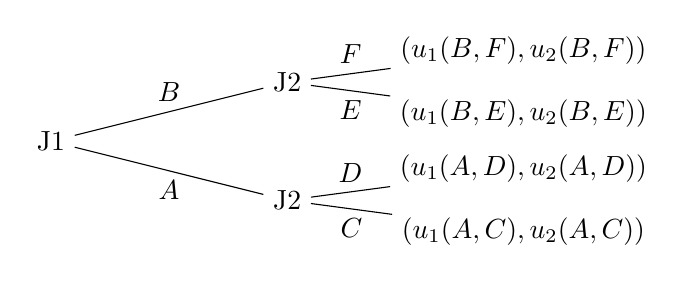
\begin{tikzpicture}[grow=right, level distance=30mm,
    level 2/.style={sibling distance=8mm}] % más distancia vertical en las hojas
\node {J1}
    child {
        node {J2}
            child { node {$(u_1(A,C),u_2(A,C))$} edge from parent node[below] {$C$}}
            child { node {$(u_1(A,D),u_2(A,D))$} edge from parent node[above] {$D$}}
            edge from parent node[below] {$A$}
    }
    child {
        node {J2}
            child { node {$(u_1(B,E),u_2(B,E))$} edge from parent node[below] {$E$}}
            child { node {$(u_1(B,F),u_2(B,F))$} edge from parent node[above] {$F$}}
            edge from parent node[above] {$B$}
    };
\end{tikzpicture}
\]

De esta forma, podemos representar las acciones de forma secuencial y los pagos a los que llega cada jugador.

En el Capítulo 3 se exponen ejemplos concretos de juegos representados de forma extensiva como el tres en raya \ref{tres_en_raya} o el ajedrez \ref{ajedrez}.

 
%Aunque vamos a detenernos en dar ejemplos de cada tipo de juego, es necesario definir dos juegos muy simples que nos ilustren ambos tipos de representación.



\section{Pero, ¿qué es realmente un juego?} \label{que_es_juego}
Definir qué es un juego puede parecer trivial a primera vista, pero se trata de una tarea sorprendentemente compleja y profundamente relevante para cualquier diseñador. La necesidad de una definición precisa no es meramente académica: no podemos aspirar a mejorar en la creación de juegos si no somos capaces de articular qué es lo que estamos diseñando. En este sentido, disponer de un vocabulario común y bien delimitado permite no solo comunicar ideas, sino también evaluar y criticar mecánicas, estructuras y experiencias lúdicas de manera rigurosa. \cite{costikyan2002}

A lo largo de la historia, distintos autores han intentado capturar la esencia del juego desde perspectivas diversas:

\subsection{Juegos como actividades culturales y sociales}

Joh Huizinga, en su influyente obra \textit{Homo Ludens} (1938) \cite{huizinga1938}, propone una definición amplia y abarcativa:

\begin{quote}
``El juego, en su aspecto formal, es una acción libre ejecutada \texttt{<<como sí>>} y sentida como situada fuera de la vida corriente, pero que, a pesar de todo, puede absorber por completo al jugador, sin que haya en ella ningún interés material ni se obtenga en ella provecho alguno, que se ejecuta dentro de un determinado tiempo y un determinado espacio, que se desarrolla en un orden sometido a reglas y que da origen a asociaciones que propenden a rodearse de misterio o a disfrazar para destacarse del mundo habitual.''
\end{quote}

Según Huizinga, el juego es:

\begin{itemize}
    \item Libre y voluntario.
    \item Desarrollado dentro de límites de tiempo y espacio.
    \item Regido por reglas.
    \item Sin finalidad práctica, es decir, un fin en sí mismo.
    \item Acompañado de tensión, alegría y separación de la vida ordinaria.
\end{itemize}

Si bien esta definición es profunda y culturalmente rica, resulta demasiado amplia para el contexto del diseño de videojuegos, ya que engloba prácticas como el teatro, rituales y otras formas de juego simbólico que no necesariamente comparten las propiedades interactivas y mecánicas de los videojuegos modernos.

\subsection{Juegos como superación de obstáculos}

Bernard Suits, en \emph{The Grasshopper: Games, Life and Utopia} (1978) \cite{suits1978}, propone un enfoque más formal y filosófico:

\begin{quote}
``Playing a game is the voluntary attempt to overcome unnecessary obstacles.''
\end{quote} 


Suits desarrolla esta definición mediante cuatro componentes fundamentales:

\begin{enumerate}
    \item Una actividad en la que los participantes intentan alcanzar un estado meta (\textit{prelusory goal}).
    \item Usando solo los medios permitidos por las reglas (\textit{lusory means}).
    \item Donde las reglas prohíben usar medios más eficaces para alcanzar la meta.
    \item Y los jugadores aceptan estas reglas precisamente porque hacen posible la actividad (\textit{lusory attitude}).
\end{enumerate}

Aunque la definición de Suits se ajusta bien a juegos de mesa o deportivos, se queda corta para capturar las dinámicas interactivas y experienciales de los videojuegos modernos, donde elementos como la narrativa, la exploración o la elección del jugador son fundamentales y no siempre encajan en la idea de ``obstáculos innecesarios''.

Esta definición resultó especialmente útil para el filósofo C. Thi Nguyen en su obra \textit{Games: Agency As Art (Thinking Art)}, donde reflexiona sobre los juegos como un medio artístico que explora la agencia humana. Nguyen reconoce desde el inicio la dificultad de proporcionar una definición satisfactoria de este fenómeno. Apoyándose en la concepción de Suits, introduce el término \textit{suitsian game} para referirse a aquellos juegos que poseen reglas formales y objetivos definidos, diferenciándolos del juego libre o abierto a la improvisación.

\subsection{La necesidad de un vocabulario para diseñar}

El artículo \textit{I Have No Words and I Must Design} \cite{costikyan2002} de Greg Costikyan aborda de manera explícita la dificultad de definir juegos y la importancia de contar con un vocabulario compartido en el diseño. Costikyan propone una definición más centrada en los elementos relevantes para el diseño:

\begin{quote}
    ``[\textit{A game is}] an interactive structure of endogenous meaning that requires players to struggle toward a goal.''
\end{quote} 


Se identifica varias propiedades que debe tener un juego:

\begin{itemize}
    \item Interacción significativa entre el jugador y el sistema.
    \item Existencia de objetivos claros.
    \item Presencia de conflictos o desafíos.
    \item Estructura y reglas que delimitan la experiencia.
    \item Significado endógeno: los jugadores entienden y valoran la experiencia desde las propias reglas.
\end{itemize}

Este enfoque permite entender mejor por qué algunas actividades, aunque entretenidas, no califican como juegos según criterios de diseño: deben ofrecer desafíos interactivos y metas que generen \textit{engagement} mediante reglas que los jugadores comprendan y acepten.

\subsection{Definición operativa}

Para los fines del diseño de videojuegos, la definición más práctica y operativa que hemos encontrado es la de Jesse Schell en \textit{The Art of Game Design: A Book of Lenses} \cite{schell2014}:

\begin{quote}
``A game is a problem-solving activity, approached with a playful attitude.''
\end{quote} 

Schell propone, a partir de un análisis comparativo de múltiples definiciones, diez cualidades esenciales que caracterizan a un juego:

\begin{enumerate}
    \item Los juegos son iniciados voluntariamente.
    \item Los juegos poseen objetivos claros.
    \item Los juegos presentan conflictos.
    \item Los juegos están regidos por reglas.
    \item Los juegos pueden ser ganados o perdidos.
    \item Los juegos son interactivos.
    \item Los juegos implican desafíos.
    \item Los juegos generan valor interno propio.
    \item Los juegos logran involucrar a los jugadores (\textit{engagement}).
    \item Los juegos constituyen sistemas formales y cerrados.
\end{enumerate}

Schell reconoce que incluso esta lista extensa puede no ser exhaustiva, y que su propósito principal es ofrecer un marco práctico para evaluar y diseñar juegos. Según el propio autor, si se necesitan muchos elementos para definir algo, probablemente convenga reagrupar y simplificar las ideas para capturar la esencia de manera más efectiva. Esta aproximación proporciona una definición operativa robusta y aplicable al diseño de videojuegos.

\hfill \break

En resumen, la literatura ha explorado diversas concepciones de juego:

\begin{itemize}
    \item Huizinga ofrece una visión cultural y social amplia, pero demasiado inclusiva para nuestro propósito.
    \item Suits formaliza la estructura de los juegos clásicos, pero no cubre del todo las particularidades de los videojuegos.
    \item Costikyan y Schell centran la definición en la interacción, el objetivo y la experiencia del jugador, proporcionando un marco útil para el diseño.
\end{itemize}

A partir de estas reflexiones, consideramos que un juego, desde la perspectiva del diseño de videojuegos, es una actividad que presenta un desafío a ser resuelto por el jugador, el cual se aborda de forma voluntaria y con intención recreativa. La definición de Schell, con sus puntos de evaluación, será nuestro punto de referencia para el análisis posterior.


\endinput
%--------------------------------------------------------------------
% FIN DEL CAPÍTULO. 
%--------------------------------------------------------------------

% !TeX root = ../tfg.tex
% !TeX encoding = utf8

\chapter{Utilidad, soluciones y equilibrio}

En el capítulo anterior se ha definido formalmente qué se entiende por un juego y sus componentes principales: el conjunto de jugadores $J$, los conjuntos de estrategias $\{S_i\}_{i\in J}$, y las funciones de pagos $\{u_i(s)\}_{i\in J}$. A partir de esta base, se introducen los conceptos de \textit{utilidad}, \textit{concepto de solución} y \textit{equilibrio}, que constituyen los pilares analíticos de la Teoría de Juegos. 

A partir de este punto se dejan de lado los aspectos de diseño para centrarse en la formalización teórica, cuya aplicación práctica se retomará posteriormente durante el desarrollo del \textit{software} (véase el capítulo \ref{cap_diseño}).

Los conceptos principales de este capítulo se basan en lo expuesto en  \textit{Teoría de Juegos} (Cerdá, Pérez y Jimeno, 2004) \cite{TeoriaDeJuegosCJP}.

\section{Utilidad}

En la Teoría de Juegos, la \textbf{utilidad} es la medida numérica que representa las preferencias o el grado de satisfacción de cada jugador respecto a los posibles resultados del juego. Dado un conjunto de resultados $X$, cada jugador $i \in J$ posee una \textbf{función de utilidad} 
\[
u_i : X \rightarrow \mathbb{R},
\]
que asigna un valor real a cada resultado $x \in X$, de manera que
\[
u_i(x') > u_i(x'') \quad \text{si y sólo si el jugador } i \text{ prefiere } x' \text{ a } x''.
\]
Esta función de utilidad puede interpretarse como una representación \textit{ordinal} de las preferencias del jugador: sólo importa el orden, no la magnitud de los valores asignados. Cualquier transformación estrictamente creciente de $u_i$ representará las mismas preferencias \cite{TeoriaDeJuegosCJP}.

En el contexto de un juego, los resultados dependen del perfil de estrategias $s$ donde:
$$s=(s_1,\dots,s_n) \in S = S_1\times \cdots \times S_n.$$ 
Así, la utilidad de un jugador se expresa como:
\[
u_i(s) = u_i(s_1, s_2, \dots, s_n),
\]
que indica lo que obtiene el jugador $i$ cuando todos los jugadores eligen las estrategias especificadas por el perfil $s$.

\subsection{Utilidad esperada}

Cuando existe incertidumbre sobre las acciones de los demás jugadores o sobre los resultados, se trabaja con \textbf{utilidades esperadas}. Si un jugador $i$ asocia una probabilidad $p(s)$ a cada perfil de estrategias $s$, la utilidad esperada se define como:
\[
\mathbb{E}[u_i] = \sum_{s \in S} p(s) \, u_i(s).
\]

Esta formulación supone que los jugadores cumplen los axiomas de racionalidad, continuidad e independencia, y permite representar sus preferencias sobre distribuciones probabilísticas de resultados mediante una función lineal en las probabilidades. En este caso, las utilidades $u_i(s)$ se denominan utilidades de Von Neumann-Morgenstern, únicas salvo una transformación afín positiva.

\section{Concepto de solución}

El objetivo de la Teoría de Juegos es identificar qué resultados pueden considerarse razonables o estables bajo el supuesto de que los jugadores actúan racionalmente. Para ello, se introducen los \textbf{conceptos de solución}, entendidos como criterios formales que permiten identificar los perfiles de estrategias más plausibles, dados los supuestos del juego \cite{TeoriaDeJuegosCJP,osborne1994course}.

El concepto de solución asocia a cada juego
\[
G = \Big\{J, \{S_i\}_{i \in J}, \{u_i(s)\}_{i \in J}\Big\}
\]
un subconjunto $S^* \subseteq S$ de perfiles de estrategias considerados razonables o estables.

Se entiende por comportamiento racional aquel orientado a maximizar la utilidad. Se asume, por tanto, que los jugadores actúan de manera racional e independiente. Aunque este supuesto no siempre se cumple en contextos reales, resulta una abstracción necesaria para poder aplicar plenamente el marco analítico de la teoría.

\subsection{Principales conceptos de solución}

Entre los conceptos de solución más relevantes se encuentran los siguientes:
\begin{itemize}
    \item \textbf{Estrategias dominantes y eliminación iterada.}  
    Se eliminan las estrategias que resultan peores que otras para el mismo jugador, independientemente de lo que hagan los demás.
    
    \item \textbf{Equilibrio de Nash.}  
    Se alcanzan perfiles de estrategias en los que ningún jugador puede mejorar su utilidad desviándose unilateralmente.
    
    \item \textbf{Óptimo de Pareto.}  
    Describe situaciones donde no se puede mejorar la utilidad de un jugador sin empeorar la de otro \cite{osborne1994course}.
    
    \item \textbf{Equilibrio bayesiano.}  
    Extiende el equilibrio de Nash a juegos con información incompleta, en los que los jugadores tienen creencias probabilísticas sobre los tipos o características de los demás.
\end{itemize}

\section{Dominación y racionalización}

Antes de buscar equilibrios, puede simplificarse el conjunto de estrategias eliminando aquellas que nunca serían elegidas racionalmente. Este proceso se conoce como \textbf{eliminación iterada de estrategias dominadas}.

\subsection{Estrategias dominadas}

Sea $S_i$ el conjunto de estrategias de un jugador $i$. Se dice que una estrategia $s_i'$ está \textbf{estrictamente dominada} por otra $s_i''$ si:
\[
u_i(s_1,...,s'_i,...,s_n) < u_i(s_1,...,s''_i,...,s_n) \quad \forall s_{j} ~|~ j\not = i.
\]
En ese caso, un jugador racional nunca elegiría $s_i'$.

Si la desigualdad es no estricta para todos los $s_{j}$ con $j\not=i$ y estricta para al menos uno, se dice que $s_i'$ está \textbf{débilmente dominada} por $s_i''$:
\[
u_i(s_1,...,s'_i,...,s_n) \le u_i(s_1,...,s''_i,...,s_n) \quad \forall s_{j} ~|~ j\not = i, \text{ con } > \text{ para algún } s_{j}.
\]

\subsection{Eliminación iterada}

La \textbf{eliminación iterada de estrategias estrictamente dominadas} consiste en:
\begin{enumerate}
    \item Eliminar de cada jugador las estrategias estrictamente dominadas.
    \item Repetir el proceso en el juego reducido.
\end{enumerate}

Si este procedimiento conduce a un único perfil de estrategias, se considera una \textbf{solución racionalizable}. En caso contrario, el conjunto restante representa las estrategias que podrían jugarse racionalmente sin contradecir la lógica de optimización individual.

\section{Equilibrio de Nash}

El \textbf{equilibrio de Nash} constituye el concepto de solución fundamental en el análisis de juegos no cooperativos. Un perfil de estrategias \( s^* = (s_1^*, \dots, s_n^*) \) constituye un equilibrio si ningún jugador puede mejorar su utilidad modificando unilateralmente su estrategia:
\[
u_i(s_1^*, \dots, s_i^*, \dots, s_n^*) \ge u_i(s_1^*, \dots, s_i, \dots, s_n^*) \quad \forall s_i \in S_i, \, \forall i \in J.
\]

\hfill \break

Vamos a introducir algunas definiciones y resultados previos que serán necesarios para enunciar y demostrar los teoremas relativos al equilibrio de Nash.

Diremos que una función \( f : S \to \mathbb{R} \) es \textbf{cuasicóncava} si, para todo par de puntos \( x, y \in S \) y para todo \( \lambda \in [0,1] \), se cumple que
\[
f(\lambda x + (1-\lambda)y) \geq \min\{f(x), f(y)\}.
\]
La cuasiconcavidad es una propiedad más débil que la concavidad, pero suficiente para asegurar que los conjuntos de mejores respuestas (es decir, los conjuntos de estrategias que maximizan la función de utilidad) sean \textbf{convexos}. Esta convexidad es un elemento clave en la demostración del teorema de existencia de equilibrio de Nash, ya que permite aplicar resultados de punto fijo (como el teorema de Kakutani).

De forma complementaria, introducimos el concepto de \textbf{correspondencia}. Diremos que una correspondencia de un conjunto \( X \) en un conjunto \( Y \) es una aplicación multivaluada \( F : X \rightrightarrows Y \) que asigna a cada elemento \( x \in X \) un subconjunto \( F(x) \subseteq Y \). A diferencia de una función ordinaria, una correspondencia puede asociar varios valores posibles a un mismo elemento de su dominio.


Por otro lado, diremos que una correspondencia \( F : X \rightrightarrows Y \) es \textbf{hemicontinua superiormente} si para toda sucesión \( \{x^k\} \subset X \) que converge a \( x \), y para toda sucesión \( \{y^k\} \subset Y \) con \( y^k \in F(x^k) \) que converge a \( y \), se cumple que \( y \in F(x) \). Intuitivamente, esta propiedad garantiza que los valores de la correspondencia no varían bruscamente ante pequeñas modificaciones de su argumento, asegurando la estabilidad de sus imágenes en el límite.

Estas nociones resultan fundamentales para aplicar el siguiente resultado, que constituye la base de la demostración del teorema de existencia de equilibrio de Nash.

\begin{teorema}[Teorema del punto fijo de Kakutani, \cite{TeoriaDeJuegosCJP}, Teorema 3.2]
Sea \( X \) un subconjunto no vacío, compacto y convexo de \( \mathbb{R}^n \), y sea \( F : X \rightrightarrows X \) una correspondencia tal que:
\begin{itemize}
    \item \( F(x) \) es no vacío, convexo y compacto para todo \( x \in X \);
    \item el grafo de \( F \) es cerrado, o equivalentemente, \( F \) es hemicontinua superiormente.
\end{itemize}
Entonces, existe al menos un punto \( x^* \in X \) tal que \( x^* \in F(x^*) \).
\end{teorema}

Este teorema garantiza la existencia de un punto fijo para correspondencias que cumplen condiciones de continuidad y convexidad, y será la herramienta central para demostrar la existencia del equilibrio de Nash en juegos continuos.

\medskip

Denotaremos por \( G \) un juego definido como:
\[
G = \Big\{J, \{S_i\}_{i \in J}, \{u_i(s)\}_{i \in J}\Big\}.
\]

A partir de los conceptos introducidos, podemos enunciar y demostrar el siguiente resultado sobre la existencia de equilibrio de Nash.

\begin{teorema}[Existencia de equilibrio de Nash en juegos continuos \cite{TeoriaDeJuegosCJP}, Teorema 3.3]
Sea \( G \) un juego en el que para cada jugador \( i \) se cumple que \( S_i \) es no vacío, compacto y convexo, y que \( u_i \) es continua en \( S \) y cuasicóncava en su propia estrategia \( s_i \). Entonces, existe al menos un equilibrio de Nash en estrategias puras.
\end{teorema}


\begin{proof}
Sea \( G \) un juego que verifica las hipótesis del teorema.  
Para cada jugador \( i \in J \), el conjunto de estrategias \( S_i \) es no vacío, compacto y convexo, y la función de utilidad \( u_i : S \to \mathbb{R} \) es continua en \( S = S_1 \times \cdots \times S_n \) y cuasicóncava en su propia estrategia \( s_i \).

Para cada jugador \( i \) definimos su correspondencia de \emph{respuesta óptima} \( R_i \), que asigna a cada perfil de estrategias \( s = (s_1, \dots, s_i, \dots, s_n) \) el conjunto de estrategias de \( i \) que son respuesta óptima a dicho perfil:
\[
R_i(s) = \left\{ x_i \in S_i \,\middle|\, u_i(s_1, \dots, x_i, \dots, s_n) \ge u_i(s_1, \dots, y_i, \dots, s_n), \, \forall y_i \in S_i \right\}.
\]

Definimos la correspondencia global de respuesta óptima \( R \) como:
\[
R(s) = R_1(s) \times \cdots \times R_n(s)
      = \left\{ t = (t_1, \dots, t_n) \in S \,\middle|\, t_i \in R_i(s), \, \forall i \in J \right\}.
\]
Esta correspondencia asigna a cada perfil de estrategias \( s \) el producto cartesiano de los conjuntos de respuesta óptima individuales.

\medskip

A continuación, comprobaremos que \( R \) cumple las condiciones del \textit{teorema del punto fijo de Kakutani}, lo que garantizará la existencia de un punto fijo \( s^* \in S \) tal que \( s^* \in R(s^*) \).

\begin{enumerate}
    \item \textbf{El conjunto \( S \) es no vacío, compacto y convexo.}  
    Por hipótesis, cada \( S_i \) cumple estas propiedades; por tanto, su producto cartesiano \( S = S_1 \times \cdots \times S_n \) también lo es.

    \item \textbf{\( R(s) \) es no vacío para todo \( s \in S \).}  
    Dado que \( u_i(\cdot) \) es continua en el conjunto compacto \( S_i \), el teorema de Weierstrass garantiza que el máximo se alcanza.  
    Por tanto, \( R_i(s) \neq \varnothing \) para cada jugador \( i \), y en consecuencia \( R(s) \neq \varnothing \).

    \item \textbf{Cada \( R(s) \) es convexo.}  
    La cuasicóncavidad de \( u_i \) respecto a su propia estrategia \( s_i \) implica que el conjunto de maximizadores \( R_i(s) \) es convexo.  
    Por tanto, el producto cartesiano \( R(s) = R_1(s) \times \cdots \times R_n(s) \) es también convexo.

    \item \textbf{La correspondencia \( R \) es hemicontinua superiormente.}  
    Sea una sucesión \( \{s^k\} \subset S \) tal que \( s^k \to s \), y una sucesión \( \{t^k\} \) con \( t^k \in R(s^k) \) y \( t^k \to t \).  
    Para cada jugador \( i \), se cumple:
    \[
    u_i(s_1^k, \dots, t_i^k, \dots, s_n^k) \ge u_i(s_1^k, \dots, y_i, \dots, s_n^k), \quad \forall y_i \in S_i.
    \]
    Al tomar el límite cuando \( k \to \infty \) y usar la continuidad de \( u_i \), se obtiene:
    \[
    u_i(s_1, \dots, t_i, \dots, s_n) \ge u_i(s_1, \dots, y_i, \dots, s_n), \quad \forall y_i \in S_i,
    \]
    de modo que \( t_i \in R_i(s) \) para todo \( i \). Por tanto, \( t \in R(s) \) y el grafo de \( R \) es cerrado, es decir, \( R \) es hemicontinua superiormente.
\end{enumerate}

Dado que \( R \) es una correspondencia definida sobre un conjunto no vacío, compacto y convexo, con valores no vacíos, convexos y un grafo cerrado, se cumplen las condiciones del \textit{teorema del punto fijo de Kakutani}.  
En consecuencia, existe \( s^* \in S \) tal que \( s^* \in R(s^*) \).

\medskip

Podemos afirmar entonces que \( R \) tiene al menos un punto fijo \( s^* = (s_1^*, \dots, s_n^*) \).  
Por tanto, \( s_i^* \in R_i(s^*) \, \forall i \in J \), es decir, \( s_i^* \) es una respuesta óptima frente a \( s^* \) para cada jugador.  
En otras palabras, \( s^* \) constituye un \textbf{equilibrio de Nash en estrategias puras} para el juego \( G \).

\end{proof}


\hfill \break

Este resultado garantiza la existencia de equilibrio en juegos con espacios de estrategias continuos, siempre que las preferencias sean bien comportadas.

Podemos aplicar este Teorema para obtener un nuevo resultado sobre juegos con estrategias mixtas.

\begin{teorema}[Existencia de equilibrio de Nash en juegos finitos \cite{TeoriaDeJuegosCJP}, Teorema 3.4] \label{T_mixtas}
En todo juego finito $G$ existe al menos un equilibrio de Nash en estrategias mixtas.
\end{teorema}

\begin{proof}
Dado el juego finito
\[
G \;=\; \{\, J,\ \{S_i\}_{i\in J},\ \{u_i\}_{i\in J}\,\},
\]
con $S_i=\{s^1_i,\dots,s^{m_i}_i\}$ finito para cada $i$, consideremos el juego $B(G)$, que tiene los mismos jugadores que $G$ y definimos como:

\smallskip

 Para cada jugador $i$, sea $B(S_i)$ el conjunto de distribuciones de probabilidad sobre $S_i$ (estrategias mixtas de $i$).  
 El espacio de perfiles mixtos es $B(S)=B(S_1)\times\cdots\times B(S_n)$.  
 Para $p=(p_1,\dots,p_n)\in B(S)$, el pago esperado de $i$ viene dado por
\[
U_i(p_1,\dots,p_n)\;=\; \sum_{s\in S}\Big(\prod_{j\in J} p_j(s_j)\Big)\,u_i(s),
\]
donde $s=(s_1,\dots,s_n)$.

\medskip
Comprobamos ahora las hipótesis del Teorema~\ref{T_mixtas} continuo (Teorema~3.3):

\begin{itemize}
  \item[(a)] Para cada $i$, $B(S_i)$ es un subconjunto no vacío, compacto y convexo de $\mathbb{R}^{m_i}$.
  \item[(b)] $U_i$ es continua en todo $B(S)$ y, fijados $p_j$ para $j\neq i$, la aplicación $p_i\mapsto U_i(p_1,\dots,p_i,\dots,p_n)$ es \emph{afín} en $p_i$; por tanto, es cuasicóncava en $p_i$.
\end{itemize}

En conclusión, por el teorema anterior, existe un equilibrio de Nash en estrategias puras para $B(G)$. Por tanto, existe un equilibrio de Nash en estrategias mixtas de $G$.

\end{proof}

Por último, vamos a enunciar, sin demostrar, un resultado importante acerca de los juegos simétricos.

\begin{teorema}[Equilibrio de Nash simétrico \cite{TeoriaDeJuegosCJP}, Teorema 3.5]
Si el juego $G$ es simétrico, donde $S_i=A$ para todo $i$, y si $A$ es compacto y convexo y las funciones $u_i$ son continuas y cuasicóncavas en su propia estrategia, entonces existe al menos un equilibrio de Nash \emph{simétrico}. Si el juego es finito, existe al menos un equilibrio de Nash simétrico en estrategias mixtas.
\end{teorema}

Los juegos simétricos son frecuentes en la economía y la biología, ya que modelan situaciones donde todos los jugadores enfrentan el mismo conjunto de estrategias y pagos estructuralmente equivalentes.


\subsection{Juegos de suma cero}

Antes de presentar un resultado clásico que conecta el equilibrio de Nash con las estrategias \textit{maximín}, conviene introducir formalmente el concepto de \textbf{juego de suma cero}.

Un juego bipersonal es de suma cero si las utilidades de ambos jugadores verifican que:
\[
u_1(s_1, s_2) + u_2(s_1, s_2) = 0 \quad \forall (s_1, s_2) \in S_1 \times S_2.
\]
Es decir, cualquier ganancia de un jugador implica una pérdida equivalente del otro.  
En este tipo de juegos el conflicto es total y los intereses de los jugadores son estrictamente opuestos.  
Por tanto, basta con analizar la función de pago de un solo jugador, ya que la del otro se deduce automáticamente como su negación.

\hfill \break
En los juegos de suma cero, cada jugador trata de optimizar su resultado bajo la hipótesis de que el adversario juega del modo más desfavorable posible.  
Así, el jugador $1$ buscará maximizar su ganancia mínima esperada:
\[
v_1 = \max_{p_1 \in \Delta(S_1)} \min_{p_2 \in \Delta(S_2)} U_1(p_1, p_2),
\]
mientras que el jugador $2$ intentará minimizar la ganancia máxima de su oponente:
\[
v_2 = \min_{p_2 \in \Delta(S_2)} \max_{p_1 \in \Delta(S_1)} U_1(p_1, p_2).
\]
Las estrategias que alcanzan esos valores se denominan, respectivamente, \textit{maximín} y \textit{minimax}.  
En general, $v_1 \le v_2$, y si ambos valores coinciden, el juego se dice que tiene un \textbf{valor} $v = v_1 = v_2$.

\vspace{1em}
En este contexto cobra especial relevancia el teorema del \textit{minimax}, resultado fundamental debido a John von Neumann, que garantiza precisamente la existencia de ese valor en todo juego finito de suma cero.  
El siguiente resultado presenta su formulación más general.

\begin{teorema}[Teorema del minimax \cite{TeoriaDeJuegosCJP}, Teorema 3.6] \label{T_minimax_neumann}
Dado un juego bipersonal finito de suma cero
\[
G = \{\{1,2\}, S_1, S_2; u_1, u_2 \},
\]
dicho juego tiene un \textbf{valor}. Es decir, existe un $v \in \mathbb{R}$ tal que $v_1 = v_2 = v$, siendo $v_1$ y $v_2$ los valores \textit{maximín} y \textit{minimax}.
\end{teorema}

\vspace{1em}
El teorema anterior establece la existencia de una situación de equilibrio en términos de expectativas:  
el jugador $1$ puede garantizarse una ganancia no inferior a $v$, mientras que el jugador $2$ puede limitar la ganancia de su adversario a lo sumo a $v$.  
El número $v$ se denomina \textbf{valor del juego} y constituye la solución natural de los juegos de conflicto puro.

\vspace{1em}
A partir de esta idea se puede establecer una conexión directa entre el equilibrio de Nash y las estrategias \textit{minimax}.  
El siguiente resultado demuestra que, en los juegos de suma cero, ambos conceptos son equivalentes: las estrategias que satisfacen la condición del teorema del \textit{minimax} son exactamente las que forman parte de los equilibrios de Nash.

\begin{teorema}[Equilibrio y estrategias \textit{minimax} \cite{TeoriaDeJuegosCJP}, Teorema 3.7] \label{T_minimax_equilibrio}
En los juegos bipersonales finitos de suma cero, las estrategias \textit{minimax} forman parte de los equilibrios de Nash, y únicamente ellas.
\end{teorema}

\begin{proof}
Sea el juego bipersonal finito de suma cero
\[
G = \{\{1,2\}, S_1, S_2; u_1, u_2 \},
\]
donde
\[
u_1(s_1, s_2) + u_2(s_1, s_2) = 0 \quad \forall (s_1, s_2) \in S_1 \times S_2.
\]
Denotemos por $A_1$ la matriz de pagos del jugador $1$, es decir,
\[
A_1 = \big(u_1(s_1, s_2)\big)_{s_1 \in S_1,\, s_2 \in S_2}, 
\qquad
A_2 = -A_1.
\]
Sean $p_1$ y $p_2$ estrategias mixtas genéricas de $1$ y $2$, es decir, distribuciones de probabilidad sobre sus respectivos conjuntos de estrategias puras.

\medskip
\textbf{(a) Si $(p_1^*, p_2^*)$ es un equilibrio de Nash, entonces $p_1^*$ y $p_2^*$ son estrategias \textit{maximín} y \textit{minimax}, y el pago corresponde al valor del juego.}

Por definición de equilibrio de Nash,
\[
U_1(p_1^*, p_2^*) = p_1^{*} A_1 p_2^{*t}
= \max_{p_1 \in \Delta(S_1)} p_1 A_1 p_2^{*t}
= \min_{p_2 \in \Delta(S_2)} p_1^{*} A_1 p_2^{t}.
\]
Denotando por $v_1$ y $v_2$ los valores \textit{maximín} y \textit{minimax} definidos como
\[
v_1 = \max_{p_1} \min_{p_2} p_1 A_1 p_2^{t}, 
\qquad
v_2 = \min_{p_2} \max_{p_1} p_1 A_1 p_2^{t},
\]
se deduce que $v_1 = v_2 = v$, por el teorema del minimax anterior.  
Por tanto,
\[
U_1(p_1^*, p_2^*) = v, \qquad U_2(p_1^*, p_2^*) = -v,
\]
y cada jugador obtiene el valor del juego.

\medskip
\textbf{(b) Recíprocamente, si $(p_1^*, p_2^*)$ son estrategias \textit{maximín} y \textit{minimax}, entonces forman un equilibrio de Nash.}

Si $p_1^*$ y $p_2^*$ alcanzan los extremos del teorema del minimax, se cumple para todo par $(p_1, p_2)$:
\[
U_1(p_1, p_2^*) \le v \le U_1(p_1^*, p_2),
\]
lo que implica que $p_1^*$ es una mejor respuesta a $p_2^*$ y viceversa.  
Por definición, $(p_1^*, p_2^*)$ constituye entonces un equilibrio de Nash.

\medskip
En resumen, en los juegos bipersonales finitos de suma cero, las estrategias \textit{maximín} y \textit{minimax} coinciden con las estrategias de equilibrio de Nash, y el valor del juego es único.
\end{proof}


\vspace{1em}
Los resultados anteriores son relevantes para el desarrollo de agentes en juego bipersonales. En capítulos posteriores (véase la Sección~\ref{minimax}) se presentará su implementación práctica, donde el algoritmo \textit{minimax} se aplica a la toma de decisiones del agente mediante exploración de árboles de juego y poda alfa–beta, buscando reproducir un comportamiento racional coherente con el valor teórico del juego.

\section{Eficiencia de Pareto}

Un perfil de estrategias $s \in S$ es \textbf{óptimo de Pareto} si no existe otro perfil $s'$ tal que:
\[
u_i(s') \ge u_i(s) \quad \forall i \in J, \quad \text{y} \quad u_j(s') > u_j(s) \text{ para algún } j \in J.
\]
Es decir, no puede mejorarse la situación de un jugador sin perjudicar a otro.  

En general, los equilibrios de Nash no son necesariamente óptimos de Pareto, como ilustra el clásico dilema del prisionero (ver sección \ref{prisionero}). La diferencia entre ambos conceptos radica en que el equilibrio de Nash se centra en la estabilidad individual, mientras que la eficiencia de Pareto mide la eficiencia social.

\section{Equilibrio bayesiano}

En los juegos con información incompleta, los jugadores desconocen ciertos elementos del entorno o de los demás. Cada jugador $i$ tiene un \textbf{tipo} $t_i \in T_i$, y una estrategia que depende de él:
\[
s_i : T_i \rightarrow S_i.
\]
Sea $p(t)$ la distribución común de probabilidad sobre los tipos $t = (t_1, \dots, t_n)$. La utilidad esperada de un jugador $i$, dado su tipo, es:
\[
\mathbb{E}_{t_{-i}}[u_i(s_i(t_i), s_{-i}(t_{-i}), t_i, t_{-i})].
\]

Un perfil $(s_1^*, \dots, s_n^*)$ constituye un \textbf{equilibrio bayesiano} si, para todo jugador $i$ y tipo $t_i$,
\[
\mathbb{E}_{t_{-i}}\!\big[u_i(s_i^*(t_i), s_{-i}^*(t_{-i}), t_i, t_{-i})\big] 
\ge 
\mathbb{E}_{t_{-i}}\!\big[u_i(s_i(t_i), s_{-i}^*(t_{-i}), t_i, t_{-i})\big],
\]
para toda estrategia alternativa $s_i$.

Este equilibrio generaliza el de Nash a entornos de información asimétrica. Su existencia se apoya, conceptualmente, en el mismo principio que el \textbf{Teorema de existencia de Nash en estrategias mixtas} (Teorema \ref{T_mixtas}), ya que los jugadores, al desconocer los tipos ajenos, deben formar distribuciones de probabilidad sobre ellos. Así, el equilibrio bayesiano puede entenderse como una extensión del equilibrio mixto de Nash al caso de incertidumbre estructurada mediante creencias probabilísticas.

Este concepto resulta fundamental en contextos como subastas, selección adversa o negociación.

\endinput
%--------------------------------------------------------------------
% FIN DEL CAPÍTULO.
%--------------------------------------------------------------------

% !TeX root = ../tfg.tex
% !TeX encoding = utf8

\chapter{Ejemplos de juegos}
Una vez establecidos los conceptos fundamentales, resulta pertinente presentar diversos ejemplos de juegos. Con el propósito de ilustrar la clasificación expuesta en el primer capítulo, se introduce un ejemplo representativo para cada categoría considerada.

\section{Juegos estáticos}
En esta sección se presentan varios juegos que ejemplifican la categoría de juegos estáticos. Se exponen dos casos clásicos y ampliamente utilizados en la literatura académica para ilustrar conceptos fundamentales: el dilema del prisionero y el mercado del limón. 
Para complementar, se muestran también algunos juegos reales, más sencillos y conocidos, que no sólo pueden modelarse dentro de este marco teórico, sino que además son jugados con fines recreativos.

\subsection{Juegos de información completa}
\subsubsection{Dilema del prisionero} \label{prisionero}

El dilema del prisionero es un ejemplo clásico y sencillo de juego de información completa.

El siguiente ejemplo está tomado textualmente de \cite{TeoriaDeJuegosCJP}, (ejemplo 2.1).

\begin{quote}
``
Dos delincuentes habituales son apresados cuando acaban de cometer un delito grave. No hay prueba clara contra ellos, pero sí indicios fuertes de dicho delito y además hay pruebas de un delito menor. Son interrogados simultáneamente en habitaciones separadas. Ambos saben que si los dos se callan serán absueltos del delito principal por falta de pruebas, pero condenados por el delito menor (1 año de cárcel), que si ambos confiesan, serán condenados por el principal pero se les rebajará un poco la pena por confesar (4 años), y finalmente, que si sólo uno confiesa, él se librará de penas y al otro «se le caerá el pelo» (5 años).''
\end{quote} 

Es claro que se trata de un juego estático, ya que ambos jugadores eligen sus estrategias de manera simultánea, sin conocer la decisión del otro. Además, es un juego de información completa, puesto que ambos jugadores conocen las estrategias disponibles y los pagos asociados a cada perfil de estrategias.

Para representarlo de forma estratégica, primero definimos el conjunto de jugadores: $$J=\{1,2\}$$ Cada jugador tiene dos estrategias disponibles:
\[
S_1=S_2=\{C,E\},
\]
donde $C$ significa ``callarse'' y $E$ significa ``entregarse''. Denotamos por $s=(s_1,s_2)$ un perfil de estrategias. Tomamos como función de pagos la negación de los años de prisión (utilidad negativa), de modo que mayores años representan peores pagos:

\[
\begin{array}{c|cc}
       & C_2 & E_2 \\ \hline
C_1    & (-1,-1) & (-5,0) \\
E_1    & (0,-5)  & (-4,-4)
\end{array}
\]

La entrada $(u_1,u_2)$ indica las utilidades de los jugadores $1$ y $2$ respectivamente. Por ejemplo, si ambos eligen $C$ reciben cada uno $-1$ (un año de prisión). Si ambos confiesan ($E,E$) reciben $-4$ (cuatro años). Si uno confiesa y el otro no, el confesor recibe $0$ y el otro $-5$.

Para cada jugador $i$ comparar las utilidades entre $C$ y $E$ muestra que $E$ es estrategia estrictamente dominante:
\begin{itemize}
    \item Si el otro juega $C$: $u_i(E, C)=0 > u_i(C, C)=-1$.
    \item Si el otro juega $E$: $u_i(E, E)=-4 > u_i(C,E)=-5$.
\end{itemize}
Por tanto el único equilibrio de Nash en estrategias puras es $(E,E)$.

El perfil $(C,C)$ es Pareto-óptimo frente a $(E,E)$ porque $-1>-4$ para ambos. Sin embargo, la estructura de incentivos lleva a ambos jugadores hacia $(E,E)$ pese a que $(C,C)$ sería mejor colectivamente. Esto ejemplifica el conflicto entre interés individual y bienestar social que caracteriza al dilema del prisionero.

\subsubsection{Piedra papel o tijeras} \label{piedra_papel_tijeras}

El juego de piedra, papel o tijeras es otro ejemplo de juego estático y de información completa, ampliamente conocido por su sencillez y simetría.

En este juego, ambos jugadores eligen simultáneamente una de las tres posibles acciones: piedra, papel o tijeras. Las reglas son bien conocidas: la piedra gana a la tijera, la tijera gana al papel y el papel gana a la piedra. Si ambos jugadores eligen la misma opción, el resultado es un empate.

Formalmente, definimos el conjunto de jugadores: $$J=\{1,2\}$$
Y los conjuntos de estrategias
\[
S_1 = S_2 = \{R, P, S\},
\]
donde $R$ representa piedra (\textit{rock}), $P$ papel (\textit{paper}) y $S$ tijeras (\textit{scissors}). Cada jugador recibe un pago de $1$ si gana, $-1$ si pierde y $0$ si empata. La matriz de pagos puede representarse del siguiente modo:

\[
\begin{array}{c|ccc}
      & R_2 & P_2 & S_2 \\ \hline
R_1   & (0,0) & (-1,1) & (1,-1) \\
P_1   & (1,-1) & (0,0) & (-1,1) \\
S_1   & (-1,1) & (1,-1) & (0,0)
\end{array}
\]

Cada entrada $(u_1,u_2)$ indica las utilidades obtenidas por los jugadores $1$ y $2$ respectivamente. Por ejemplo, si el jugador 1 elige piedra y el jugador 2 tijeras, el primero gana y obtiene $1$, mientras que el segundo pierde y obtiene $-1$.

Cada entrada $(u_1,u_2)$ indica las utilidades obtenidas por los jugadores $1$ y $2$, respectivamente. Por ejemplo, si el jugador 1 elige piedra y el jugador 2 tijeras, el primero gana y obtiene $1$, mientras que el segundo pierde y obtiene $-1$.

Observamos que este juego no posee un equilibrio de Nash en estrategias puras, ya que para cualquier combinación determinista alguno de los jugadores puede mejorar su resultado cambiando unilateralmente su elección. Formalmente, para cualquier par $(s_1,s_2) \in S_1 \times S_2$, existe una desviación $s_1' \in S_1$ tal que:
\[
u_1(s_1',s_2) > u_1(s_1,s_2),
\]
y de modo análogo para el jugador $2$.

Sin embargo, existe un equilibrio en estrategias mixtas, en el que cada jugador elige piedra, papel o tijeras con igual probabilidad $\frac{1}{3}$.

En este caso, en lugar de trabajar con estrategias puras, consideramos funciones de distribución de probabilidad sobre $S_i = \{R, P, S\}$:
\[
\sigma_i(s)=
\begin{cases}
    p_r & \text{si } s=R, \\
    p_p & \text{si } s=P, \\
    p_s & \text{si } s=S.
\end{cases}
\]
Las funciones de utilidad esperada vienen dadas por:
\[
\mathbb{E}[u_i(\sigma_1,\sigma_2)]
\]
donde la esperanza se calcula sobre las distribuciones de probabilidad de ambos jugadores.

Podemos tomar la distribución que asigna la misma probabilidad a cada estrategia:
\[
\sigma_i^*(s)=
\begin{cases}
    \frac{1}{3} & \text{si } s=R, \\
    \frac{1}{3} & \text{si } s=P, \\
    \frac{1}{3} & \text{si } s=S.
\end{cases}
\]

La utilidad esperada para cada jugador viene dada por:
\[
\mathbb{E}[u_i(\sigma_1,\sigma_2)] = \sum_{s_1\in S_1}\sum_{s_2\in S_2} \sigma_1(s_1)\sigma_2(s_2)\,u_i(s_1,s_2).
\]
Sustituyendo las distribuciones uniformes, obtenemos:
\[
\mathbb{E}[u_i(\sigma_1^*,\sigma_2^*)]=0 \qquad \forall i\in J.
\]

Este perfil de estrategias mixtas constituye un equilibrio de Nash, ya que ningún jugador puede mejorar su utilidad esperada mediante una desviación unilateral:
\[
\mathbb{E}[u_i(\sigma_1^*,\sigma_{2}^*)] \ge \mathbb{E}[u_i(\sigma_1,\sigma_{2}^*)] \qquad \forall \sigma_1 \in \Delta(S_1)
\]
donde $\Delta(S_1)$ denota el conjunto de distribuciones de probabilidad sobre el conjunto de estrategias puras $S_1$. El mismo razonamiento es válido para el jugador $2$.

En este equilibrio, cada jugador selecciona piedra, papel o tijeras con igual probabilidad, de modo que el juego permanece perfectamente simétrico y de suma cero. Así, piedra, papel o tijeras constituye un ejemplo clásico de equilibrio mixto en un juego competitivo simple.


\hfill \break

El estudio de juegos como piedra, papel o tijeras resulta especialmente útil porque ejemplifica un patrón de relaciones cíclicas de ventaja/desventaja que aparece en muchos sistemas lúdicos reales. En efecto, numerosos subsistemas de juegos más complejos se fundamentan en equilibrios similares, en los que distintas categorías interactúan mediante ventajas y debilidades recíprocas. Por ejemplo, esta estructura está presente en los tipos elementales de \textit{Pokémon} \cite{wrpsa_pokemon} y en los roles o tipos de campeones en los juegos \textit{MOBA} (Massive Online Battle Arena), donde cada tipo puede tener ventaja frente a uno y desventaja frente a otro, generando una dinámica de contrarrestes mutuos. \cite{80lv_rps_strategy, wrpsa_modern_games}
%lidia este parrafo es super importante me querrias

%\subsubsection{Penalti}
%Tirar un penalti
%y yo aqui pongo que esto es inutil y es que me gusta pensar en cosas o eso me lo guardo?

\subsection{Juegos de información incompleta}
\subsubsection{Mercado del limón} \label{limon}
El mercado del limón es un ejemplo clásico de juego de información incompleta, introducido por George Akerlof en su artículo \textit{The Market for ``Lemons``} \cite{akerlof1970lemons}. Este modelo ilustra cómo la asimetría de información puede provocar un fallo de mercado.

\begin{quote}
Supongamos un mercado de automóviles usados en el que hay dos tipos de coches: malos y buenos (llamados ``limones`` y ``melocotones`` respectivamente). Los vendedores conocen la calidad real de su coche, pero los compradores no pueden distinguir entre un coche bueno y uno malo antes de la compra. Ambos saben, sin embargo, la proporción de coches buenos y malos en el mercado, así como los valores medios esperados.
\end{quote}

En este contexto, la información sobre la calidad del coche no es completa: los vendedores conocen más que los compradores. Por tanto, el juego presenta información incompleta.

Podemos representarlo de manera simplificada como un juego estático de tipo bayesiano con dos jugadores:
\[
J=\{\text{Vendedor}, \text{Comprador}\}.
\]

El vendedor puede tener dos tipos posibles:
\[
T_{\text{Vendedor}} = \{\text{Melocotón}, \text{Limón}\}.
\]
El comprador no conoce el tipo del vendedor, pero tiene una creencia inicial sobre la probabilidad de que el coche sea bueno o malo. Denotamos estas probabilidades por $p$ y $1-p$, respectivamente.

Las estrategias posibles son:
\[
S_{\text{Vendedor}} = \{\text{Ofrecer}, \text{No ofrecer}\}, \quad S_{\text{Comprador}} = \{\text{Comprar}, \text{No comprar}\}.
\]

Si el comprador adquiere un coche bueno, su utilidad neta es el valor del coche $v_b$ menos el precio $p_c$. Si compra un coche malo, obtiene $v_m - p_c$, con $v_m < v_b$. Para el vendedor, el pago depende del precio recibido menos su valoración del coche.

Debido a la asimetría de información, el comprador anticipa que, a cualquier precio intermedio, los vendedores de coches buenos tendrán menos incentivo para vender que los de coches malos. Esto reduce la calidad esperada de los coches ofertados y, en equilibrio, puede hacer que desaparezca el mercado: sólo se venden coches malos.

En resumen, el \textit{mercado del limón} muestra cómo la falta de información simétrica puede generar un equilibrio ineficiente, en el que las transacciones potencialmente mutuamente beneficiosas no se llevan a cabo. Este resultado pone de manifiesto que la información incompleta puede alterar de forma sustancial el equilibrio de un mercado.

Los sistemas de apuestas resultan de gran interés tanto en contextos económicos reales como en el diseño de juegos de mesa modernos. En particular, constituyen una mecánica habitual dentro del género de los \textit{Eurogames}. Este subgénero se caracteriza, entre otros aspectos, por priorizar la solidez mecánica frente a la temática y por propiciar formas de interacción más sutiles entre los jugadores, basadas en el conflicto indirecto, lo que explica la popularidad de las mecánicas de pujas y apuestas \cite{eurogames2012}. Algunos diseñadores de reconocido prestigio, como Reiner Knizia (matemático de formación y autor de más de setecientos juegos publicados), incorporan principios relacionados con el equilibrio bayesiano en los mecanismos de pujas y puntuación, con el objetivo de generar sistemas estratégicamente ricos y dinámicos \cite{knizia_tlagd}.

\subsubsection{Póker a una ronda o \textit{Kuhn}}\label{poker_una_ronda}

El póker a una ronda, también conocido como \textit{Kuhn poker}, constituye un ejemplo paradigmático de juego con información incompleta y componente estratégico de engaño, ampliamente estudiado en la Teoría de Juegos como modelo de interacción con información privada y señales. A diferencia de juegos como el dilema del prisionero o piedra, papel o tijeras, aquí los jugadores no disponen de información completa sobre el estado del juego, lo que introduce incertidumbre y estrategias mixtas basadas en probabilidades y credibilidad.

\begin{quote}
Consideremos un juego simplificado de póker entre dos jugadores. Cada uno recibe una carta del mazo, la cual puede ser alta (A) o baja (B), con igual probabilidad. El valor de la carta es conocido solo por el jugador que la recibe. A continuación, el jugador 1 puede apostar (subir) o pasar. Si pasa, el jugador 2 también pasa y ambos muestran sus cartas: gana el jugador con la carta más alta. Si el jugador 1 apuesta, el jugador 2 puede retirarse o igualar la apuesta. Si se retira, el jugador 1 gana automáticamente; si iguala, ambos muestran sus cartas y el jugador con la carta más alta gana el bote \cite{sklansky1994theory}.
\end{quote}

Este escenario es un juego de información incompleta, ya que cada jugador conoce su propia carta pero desconoce la del oponente. La incertidumbre sobre la mano del rival da lugar a estrategias de \textit{bluffing} (faroles), en las cuales un jugador con una carta baja puede apostar intentando hacer creer al otro que posee una carta alta.

Formalmente, podemos definir el juego como:
\[
J = \{1,2\}, \quad T_i = \{\text{Alta}, \text{Baja}\} \text{ para } i=1,2.
\]

Cada jugador conoce su tipo, pero desconoce el del rival. Las estrategias disponibles son:
\[
S_1 = \{\text{Apostar si Alta}, \text{Apostar si Baja}, \text{Pasar}\}, \quad
S_2 = \{\text{Igualar}, \text{Retirarse}\}.
\]

El póker a una ronda es un juego bayesiano simple: cada jugador dispone de información privada (su carta) y toma decisiones estratégicas en función de sus creencias sobre el oponente. En equilibrio bayesiano, las estrategias suelen ser mixtas e incluyen, ocasionalmente, apuestas con manos débiles (faroles) para preservar la incertidumbre. No obstante, la forma concreta del equilibrio depende críticamente de los parámetros del modelo, como la probabilidad \textit{ex ante} de cada tipo y el tamaño relativo de las apuestas. \cite{osborne1994course}

Este modelo, formulado originalmente por John C. Harsanyi como ejemplo de juego bayesiano, muestra cómo la información privada y las estrategias de señalización pueden influir de manera decisiva en el resultado del juego \cite{harsanyi1967games1}.

\section{Juegos dinámicos}
En esta sección se presentan diversos juegos que ilustran la categoría de juegos dinámicos. Los ejemplos seleccionados no solo poseen relevancia en la literatura académica, sino que también constituyen elecciones populares en contextos recreativos y competitivos.

\subsection{Juegos de información completa}

\subsubsection{Tres en raya} \label{tres_en_raya}

El tres en raya es un ejemplo clásico de juego de información completa, finito y determinista. Ambos jugadores observan todas las jugadas y conocen exactamente el estado del tablero en cada momento.

\begin{quote}
Dos jugadores, $X$ y $O$, alternan turnos colocando su símbolo en una cuadrícula de $3\times3$. Gana quien consiga alinear tres de sus símbolos en fila, columna o diagonal. Si todas las casillas se llenan sin que nadie consiga alinear tres, el juego termina en empate.
\end{quote}

Podemos representar el juego en forma extensiva, donde cada nodo corresponde a un estado del tablero y cada rama a una jugada posible. Dado que ambos jugadores observan el tablero completo, no hay información oculta.

En términos formales:
\[
J = \{X, O\}, \quad S_X, S_O = \text{conjunto de secuencias posibles de movimientos válidos.}
\]

Los pagos se definen como:
\[
u_X =
\begin{cases}
1 & \text{si $X$ gana},\\
0 & \text{si hay empate},\\
-1 & \text{si $O$ gana,}
\end{cases}
\qquad
\]
\[
 u_O = -u_X.
\]
%hago un ejemplo de partida que termine emn empate representado en arbol?

La representación en forma extensiva permite visualizar las decisiones secuenciales y el carácter de información perfecta del juego. En la Figura~\ref{fig:tictactoe_extensivo} se muestra un fragmento del árbol de decisión correspondiente al tres en raya.

\begin{figure}[h]
\centering
\includegraphics[width=1\textwidth]{img/tres_en_ralla_arbol.PNG}
\caption{Representación parcial en forma extensiva del juego de tres en raya. Creación propia.}
\label{fig:tictactoe_extensivo}
\end{figure}

%no he definido lo que es suma cero y simétrico, debería hacerlo en lo de tipos de juegos?
El juego es de suma cero y simétrico. Su análisis permite determinar estrategias dominantes y soluciones mediante retroinducción. De hecho, se sabe que, con juego perfecto de ambos lados, el resultado siempre será un empate. El tres en raya ilustra un caso de equilibrio de Nash puro, alcanzado cuando ninguno de los jugadores puede mejorar su resultado cambiando unilateralmente de estrategia.

Resulta pertinente retomar las definiciones expuestas en la sección \ref{que_es_juego}, pues el tres en raya constituye un ejemplo limítrofe entre el concepto de ``juego'' y el de ``puzzle''. Dado que posee un equilibrio perfectamente definido: en el que, al jugar de forma óptima, la partida siempre concluye en empate. La interacción estratégica y la resolución de problemas son prácticamente inexistentes. No obstante, para jugadores que desconocen dicha estrategia óptima, como puede ser el caso de los niños pequeños, el tres en raya sí cumple las condiciones necesarias para ser considerado un juego. Este ejemplo pone de manifiesto que la naturaleza lúdica depende tanto de la experiencia del jugador como del sistema de reglas en sí. \cite{nguyen2020}


\subsubsection{Ajedrez} \label{ajedrez}

El ajedrez es otro ejemplo representativo de juego de información completa, aunque con una complejidad combinatoria mucho mayor que el tres en raya. En este caso, los jugadores también observan completamente el tablero, las piezas y los movimientos posibles del adversario.

\begin{quote}
Dos jugadores, Blancas y Negras, alternan turnos moviendo sus piezas sobre un tablero de $8\times8$ siguiendo reglas bien definidas. El objetivo es dar jaque mate al rey contrario, es decir, situarlo bajo amenaza de captura sin posibilidad de escape.
\end{quote}
%explico al detalle las reglas del ajedrez?

Formalmente:
\[
J = \{\text{Blancas}, \text{Negras}\}, \quad S_i = \text{conjunto de secuencias legales de movimientos.}
\]

Los pagos pueden definirse como:
\[
u_{\text{Blancas}} =
\begin{cases}
1 & \text{si Blancas ganan},\\
0 & \text{si hay tablas},\\
-1 & \text{si Negras ganan,}
\end{cases}
\qquad
\]
\[
u_{\text{Negras}} = -u_{\text{Blancas}}.
\]

Aunque el ajedrez es teóricamente resoluble por ser un juego finito de información perfecta, su tamaño hace inviable el cálculo completo de la forma extensiva o del árbol de decisión. Sin embargo, la teoría garantiza que existe un equilibrio de Nash en estrategias puras: una secuencia de jugadas óptimas para ambos jugadores que determina el resultado final (victoria de uno o tablas).

El ajedrez es, por tanto, un ejemplo paradigmático de cómo los juegos de información completa pueden ser analizados mediante los principios de la Teoría de Juegos, aunque su resolución práctica requiera aproximaciones computacionales o heurísticas.

\subsection{Juegos de información incompleta}

\subsubsection{Póker Texas Hold’em}\label{poker_holdem}
El \textit{Texas Hold’em} es la variante de póker más popular tanto en entornos recreativos como competitivos. Se trata de un juego de información incompleta, en el que cada jugador dispone de información privada (sus cartas ocultas) y de información pública (las cartas comunitarias visibles por todos). El desarrollo secuencial de las apuestas genera un espacio de decisión extenso que combina incertidumbre y estrategia probabilística.

\begin{quote}
El juego utiliza una baraja estándar de 52 cartas y puede involucrar entre dos y diez jugadores. Cada uno recibe dos cartas privadas, conocidas como \textit{hole cards}, mientras que cinco cartas comunitarias se revelan progresivamente en el centro de la mesa. Los jugadores forman su mejor mano de cinco cartas combinando sus dos cartas privadas con las cinco comunitarias.
\end{quote}

Cada ronda de \textit{Texas Hold’em} se compone de las siguientes fases \cite{harlan2006dummies}:

\begin{enumerate}
\item \textbf{Apuestas iniciales y ciegas.} Antes de repartir las cartas se colocan dos apuestas forzadas: la \textit{ciega pequeña} (\textit{small blind}) y la \textit{ciega grande} (\textit{big blind}). Estas apuestas garantizan la existencia de un bote inicial e introducen incentivos estratégicos desde el primer momento.
\item \textbf{Pre-flop.} Cada jugador recibe sus dos cartas privadas y decide si retirarse (\textit{fold}), igualar la apuesta (\textit{call}) o subir (\textit{raise}).
\item \textbf{Flop.} Se descubren tres cartas comunitarias boca arriba. Tiene lugar una nueva ronda de apuestas en la que los jugadores actualizan sus creencias sobre la fuerza de su mano.
\item \textbf{Turn.} Se revela una cuarta carta comunitaria, seguida de otra ronda de apuestas.
\item \textbf{River.} Se muestra la quinta carta comunitaria y se realiza la última ronda de apuestas.
\item \textbf{Showdown.} Si quedan varios jugadores activos, muestran sus cartas privadas y gana quien tenga la mejor combinación de cinco cartas.
\end{enumerate}

\paragraph{Ejemplo.}
Consideremos una mano simplificada entre tres jugadores: A, B y C. Las ciegas son de 50 y 100 fichas, y el juego es \textit{No-Limit}.
\begin{itemize}
\item A recibe As\spade{} y 10\heart{}, B recibe 7\club{} y 7\diamondcard{}, C recibe K\club{} y 9\spade{}.
\item En el pre-flop, A sube a 300 fichas, B iguala y C se retira.
\item En el \textit{flop} (10\diamondcard{}, 7\spade{}, 3\club{}), B obtiene un trío de sietes y A una pareja de dieces. A apuesta 400 fichas y B iguala.
\item En el \textit{turn} (Q\club{}), B mantiene la ventaja.
\item En el \textit{river} (10\club{}), A mejora a trío de dieces y gana la mano, obteniendo todas las fichas apostadas.
\end{itemize}

Este ejemplo ilustra cómo la información incompleta y las apuestas sucesivas inducen comportamientos estratégicos complejos: faroles, semifaroles, gestión del riesgo y deducción probabilística del rango del oponente.

Siguiendo la formulación de Harsanyi para juegos bayesianos \cite{harsanyi1967games1}, en el \textit{Texas Hold’em} se identifican los siguientes elementos:
\[
J = \{1,2,\dots,n\},
\]
donde $n$ es el número de jugadores.

Cada jugador $i$ recibe un tipo privado $t_i \in T_i$, que corresponde a sus dos cartas iniciales (\textit{hole cards}). La distribución de tipos está dada por una probabilidad comúnmente conocida por combinatoria,
%\[
%p(t_1, \dots, t_n) = \frac{1}{\binom{52}{2}\binom{50}{2}\dots\binom{52-2(n-1)}{2}},
%\]
lo que garantiza información común sobre la estructura del azar.

Las estrategias puras de un jugador $i$ pueden definirse como funciones:
\[
s_i : T_i \times H_i \rightarrow A_i,
\]
donde $H_i$ representa el historial público de apuestas y cartas reveladas, y $A_i$ el conjunto de acciones posibles en cada ronda: $A_i={\text{retirarse}, \text{igualar}, \text{subir}}$.

Los pagos $u_i$ dependen del resultado final (la mejor mano de cinco cartas y el tamaño del bote) y se distribuyen como:
\[
u_i(s_1, \dots, s_n, t_1, \dots, t_n) =
\begin{cases}
b_i, & \text{si el jugador $i$ gana el bote},\\
-b_i', & \text{si pierde la mano},\\
0, & \text{en caso de empate.}
\end{cases}
\]

El equilibrio de Bayes-Nash se alcanza cuando cada jugador elige su estrategia óptima dada su información privada y las creencias sobre las estrategias de los demás.

\hfill \break
El \textit{Texas Hold’em} combina información privada, azar y señales públicas en una estructura secuencial. Su análisis dentro de la Teoría de Juegos permite estudiar conceptos como la actualización bayesiana de creencias, la racionalidad limitada y el equilibrio estratégico bajo incertidumbre. Por ello, constituye uno de los modelos más utilizados en la investigación sobre decisión estratégica y Teoría de Juegos aplicada a la economía del comportamiento \cite{chen2006poker}.

\subsubsection{Magic: The Gathering}

\textit{Magic: The Gathering} (MTG) \footnote{A partir de ahora usaremos MTG para referirnos a \textit{Magic: The Gathering}} \cite{mtg} es un \textit{trading card game} (TCG)\footnote{A partir de ahora usaremos TCG para referirnos a los \textit{trading card games}} o juego de cartas coleccionables de temática fantástica cuyo objetivo consiste en derrotar al oponente reduciendo sus puntos de vida a cero mediante el uso de criaturas, conjuros y encantamientos. Diseñado en 1993 por Richard Garfield \cite{bbg_richard}, MTG fue el título que popularizó el género y estableció muchas de las bases mecánicas que aún hoy definen los TCG. Su influencia en el diseño moderno de juegos de mesa y cartas es incuestionable: resulta difícil encontrar un diseñador que no cite \textit{Magic: The Gathering} como una de sus principales referencias, o un jugador que no haya oído hablar de él. \cite{garfield_tlagd}

Los trading card games (TCCG o TCG) son juegos de cartas en los que los participantes construyen sus propios mazos a partir de una amplia colección de cartas con diferentes habilidades, valores y funciones. Estas cartas suelen obtenerse mediante sobres aleatorios o intercambios entre jugadores, lo que introduce un componente económico y de coleccionismo además del estratégico. El diseño de un TCG combina gestión de recursos, construcción de mazos y toma de decisiones tácticas, generando una profundidad de juego que equilibra azar y habilidad.

En el caso de MTG, en su modalidad \textit{standard}, dos jugadores se enfrentan con mazos de al menos 60 cartas y una reserva inicial de 20 puntos de vida. El desarrollo de la partida se organiza en turnos compuestos por varias fases: mantenimiento, principal y combate. En los que los jugadores pueden desplegar criaturas, lanzar conjuros o activar habilidades. Uno de los elementos más característicos del sistema de reglas es la gestión del maná, recurso con el que se pagan los costes de las cartas. Este se obtiene de las cartas de \textit{Tierra}, que se pueden jugar una por turno y deben “girarse” para generar maná de distintos colores. La correcta administración de este recurso determina las acciones disponibles en cada turno y condiciona la estrategia general, ya que las cartas más poderosas exigen mayores cantidades o combinaciones específicas de maná \cite{ganivet2024}.

MTG combina elementos de información incompleta, el contenido del mazo y la mano de cada jugador permanecen ocultos, con un marcado componente de planificación previa, representado por la construcción del mazo o \textit{deckbuilding}. Esta doble dimensión, estratégica y táctica, genera un espacio de decisión extenso y altamente complejo. Según Ganivet et al. \cite{ganivet2024}, la estructura secuencial y la dependencia contextual de las decisiones hacen de MTG un entorno idóneo para el estudio de la inteligencia artificial y la optimización heurística, ya que el número de posibles configuraciones supera ampliamente cualquier capacidad de cálculo exhaustivo.

En consecuencia, MTG puede considerarse un juego con múltiples equilibrios dinámicos, donde las estrategias óptimas dependen del contexto: composición del mazo, tipo de oponente y evolución de la partida. Los estudios recientes demuestran que incluso agentes basados en reglas o algoritmos evolutivos tienden a converger hacia comportamientos \textit{cuasi–óptimos} sin alcanzar un equilibrio estable en el sentido clásico. Esta propiedad lo convierte en un modelo de referencia para el análisis de sistemas con información oculta y toma de decisiones secuencial. En nuestro caso, el paralelismo con MTG es directo: el jugador debe gestionar información incompleta, optimizar recursos limitados y equilibrar riesgo y recompensa dentro de un entorno con resultados parcialmente impredecibles. \cite{urzagpt2025}



% https://www.sciencedirect.com/science/article/pii/S1875952125000771
% https://ceur-ws.org/Vol-3599/paper_4.pdf

\endinput
%--------------------------------------------------------------------
% FIN DEL CAPÍTULO. 
%--------------------------------------------------------------------

% !TeX root = ../tfg.tex
% !TeX encoding = utf8

\chapter{Algoritmos para IA en juegos} \label{algoritmos}
Una vez expuestos los distintos tipos de juegos y sus características fundamentales, el siguiente paso consiste en analizar los mecanismos mediante los cuales pueden ser jugados o resueltos. Si bien algunos juegos permiten identificar soluciones de equilibrio de forma analítica, en otros casos resulta necesario recurrir a agentes capaces de determinar y ejecutar estrategias de manera autónoma.
El estudio de estos agentes permite aproximarse a la resolución de juegos complejos, incluso cuando no es posible obtener una solución exacta. En tales situaciones, el objetivo pasa a ser el diseño de agentes que actúen de forma racional dentro del entorno del juego, optimizando su comportamiento.

\section{Agentes}
En inteligencia artificial, un \textbf{agente} es una entidad que percibe su entorno mediante sensores y actúa sobre él a través de actuadores \cite{RussellNorvig2021}. El comportamiento del agente está determinado por una función agente que asigna una acción a cada secuencia posible de percepciones.
Un \textbf{agente racional} elige las acciones que maximicen su medida de rendimiento esperada, en función de las percepciones y el conocimiento disponible.


Según su complejidad, pueden distinguirse agentes reactivos simples, basados en modelos, basados en objetivos y basados en utilidad. Cada tipo amplía la capacidad del agente para razonar sobre el entorno, planificar y adaptarse, acercándose a un comportamiento racional en contextos dinámicos e inciertos.

\section{Algoritmos para juegos con información completa} 
Esta sección se basa en los contenidos de \textit{Inteligencia Artificial: Un enfoque moderno} (Russell, Stuart J. and Norvig, Peter, 2022) \cite{RussellNorvig2021}.

Los algoritmos que se presentan a continuación suponen un entorno competitivo de juego de suma cero, tal como se definió en la sección anterior y se analizó en el \textit{Teorema de equilibrio y estrategias minimax} (Teorema \ref{T_minimax_equilibrio}). En este tipo de juegos, las ganancias de un jugador equivalen exactamente a las pérdidas del otro, por lo que el análisis puede realizarse desde la perspectiva de un único jugador: maximizar su utilidad implica simultáneamente minimizar la de su oponente.


\subsection{Minimax} \label{minimax}
El algoritmo \textbf{minimax} constituye la base de la toma de decisiones óptima en juegos secuenciales de información completa con suma cero. Su objetivo es determinar la estrategia que maximiza la ganancia mínima posible del jugador, asumiendo que el oponente juega de forma perfecta.

Sea un juego representado de forma extensiva por un árbol de decisión en el que los nodos representan estados $n$ y los arcos representan acciones posibles. Los nodos terminales están asociados a valores de utilidad \( u(s) \), que cuantifican el resultado final para el jugador maximizador. En cada nivel del árbol, los jugadores alternan su turno:
\begin{itemize}
    \item El jugador \textbf{MAX} elige la acción que \textbf{maximiza} el valor esperado.
    \item El jugador \textbf{MIN} elige la acción que \textbf{minimiza} dicho valor, buscando reducir la ganancia del rival.
\end{itemize}

Formalmente, el valor de un estado \( n \) se define recursivamente como:
\[
V(n) =
\begin{cases}
u(n) & \text{si $n$ es terminal},\\
\max\limits_{s \in \text{Sucesores}(n)} V(s) & \text{si $n$ es un estado de MAX},\\
\min\limits_{s \in \text{Sucesores}(n)} V(s) & \text{si $n$ es un estado de MIN}.
\end{cases}
\]

Llamamos a \( V(n) \) el \textbf{valor minimax} del nodo \( n \).  
Si \( n \) es un nodo terminal, \( u(n) \) representa la utilidad asociada al resultado alcanzado siguiendo la secuencia de decisiones que conduce hasta \( n \).

De esta forma, el algoritmo explora el árbol de juego hasta las hojas y propaga hacia arriba los valores de utilidad, seleccionando en la raíz la acción con el valor máximo.

\hfill \break
El agente que aplica el algoritmo minimax puede interpretarse como un agente basado en modelos, ya que mantiene una representación explícita del entorno del juego (el árbol de estados) y razona sobre él para seleccionar la acción óptima.
Este agente asume que el oponente también actúa racionalmente, maximizando su propia utilidad, lo que lo convierte en un agente racional en el sentido definido al inicio del capítulo.

\subsubsection{Minimax en el tres en raya.}

Se desarrolla ahora el caso del tres en raya, definido anteriormente.

Un agente minimax para este juego actúa de la siguiente forma:
\begin{enumerate}
    \item Genera todos los movimientos posibles desde el estado actual.
    \item Evalúa los estados terminales según la función de utilidad definida.
    \item Propaga los valores hacia atrás aplicando las reglas de maximización y minimización.
    \item Selecciona el movimiento con el valor \( V(s) \) máximo.
\end{enumerate}

La representación en forma extensiva permite visualizar las decisiones secuenciales y el carácter de información perfecta del juego. En la Figura~\ref{fig:tres_en_raya_minimax} se muestra un fragmento del árbol de decisión correspondiente a una partida que termina en empate. Cada nodo alterna entre decisiones de MAX (X) y MIN (O), y las utilidades en las hojas determinan la estrategia óptima.

\begin{figure}[H]
\centering
\includegraphics[width=\textwidth]{img/Minimax_tres_en_raya.png}
\caption{Un árbol (parcial) de búsqueda minimax para el juego de tres en raya. Creación propia.}
\label{fig:tres_en_raya_minimax}
\end{figure}


%induccion hacia atras
%induccion hacia atras generalizada
%\subsection{Negamax}
\subsection{Poda \(\alpha\)-\(\beta\)} %revisar

La poda \(\alpha\)-\(\beta\) es una optimización del algoritmo minimax que reduce el número de nodos evaluados sin alterar el resultado final óptimo. Se basa en el hecho de que, en muchos casos, es posible detectar que cierta rama del árbol no puede cambiar la decisión definitiva y descartarla anticipadamente.  

La poda $\alpha-\beta$ debe su nombre de los dos parámetros que describen los umbrales sobre los valores hacia atrás que aparecen durante la exploración:
\begin{itemize}
    \item \(\alpha\): el valor (máximo) garantizado hasta ahora para el jugador MAX.
    \item \(\beta\): el valor (mínimo) garantizado hasta ahora para el jugador MIN.
\end{itemize}

La poda $\alpha-\beta$ actualiza el valor de $\alpha$ y $\beta$ según se va explorando el árbol y poda (es decir, deja de recorrer), las ramas restantes en un nodo en el momento en el valor del nodo actual es peor que el actual valor $\alpha$ o $\beta$ para MAX o MIN, respectivamente.

Formalmente, la función recursiva se puede escribir como:

\[
\text{AlphaBeta}(n, \alpha, \beta) =
\begin{cases}
u(n), & \text{si } n \text{ es terminal}, \\
\max\limits_{s \in \text{Sucesores}(n)} \text{AlphaBeta}(s, \alpha, \beta), & \text{si turno = MAX}, \\
\min\limits_{s \in \text{Sucesores}(n)} \text{AlphaBeta}(s, \alpha, \beta), & \text{si turno = MIN},
\end{cases}
\]

pero con las condiciones de poda:

\begin{itemize}
    \item En el caso MAX: cuando calculamos un sucesor \(s\) y obtenemos un valor \(v = \text{AlphaBeta}(s, \alpha, \beta)\), si \(v > \alpha\) actualizamos \(\alpha = v\). Si en algún momento \(\alpha \ge \beta\), rompemos el bucle de sucesores (corte).
    \item En el caso MIN: cuando obtenemos un sucesor con valor \(v\), si \(v < \beta\) actualizamos \(\beta = v\). Si \(\beta \le \alpha\), hacemos corte (podar).
\end{itemize}

El agente que utiliza poda $\alpha-\beta$ mantiene el mismo tipo de racionalidad que el agente minimax, pero optimiza su proceso de decisión reduciendo la cantidad de estados explorados. Se trata, por tanto, de un agente basado en modelos que emplea un mecanismo de búsqueda más eficiente para alcanzar decisiones racionales en tiempo finito.

Es por esto que se utiliza ampliamente para juegos complejos bipersonales de suma cero, como el ajedrez o el tres en raya.


\subsubsection{El algoritmo de búsqueda $\alpha-\beta$}

\begin{algorithm}[H]
\caption{Búsqueda Alfa–Beta (adaptado de \cite{RussellNorvig2021}).}
\label{alg:alphabeta}
\begin{algorithmic}[1]
\Function{BÚSQUEDA-ALFA-BETA}{estado}
    \State \textbf{entrada:} estado, estado actual del juego
    \State $v \gets$ \Call{MAX-VALOR}{estado, $-\infty$, $+\infty$}
    \State \Return la acción de \textsc{Sucesores}$(estado)$ con valor $v$
\EndFunction
\vspace{0.5em}
\Function{MAX-VALOR}{estado, $\alpha$, $\beta$}
    \State \textbf{entrada:} estado, $\alpha$ valor de la mejor alternativa para MAX, $\beta$ para MIN
    \If{\Call{TEST-TERMINAL}{estado}}
        \State \Return \Call{UTILIDAD}{estado}
    \EndIf
    \State $v \gets -\infty$
    \ForAll{$s$ en \textsc{Sucesores}$(estado)$}
        \State $v \gets \max(v, \Call{MIN-VALOR}{s, \alpha, \beta})$
        \If{$v \geq \beta$} \Return $v$ \EndIf
        \State $\alpha \gets \max(\alpha, v)$
    \EndFor
    \State \Return $v$
\EndFunction
\vspace{0.5em}
\Function{MIN-VALOR}{estado, $\alpha$, $\beta$}
    \State \textbf{entrada:} estado, $\alpha$ valor de la mejor alternativa para MAX, $\beta$ para MIN
    \If{\Call{TEST-TERMINAL}{estado}}
        \State \Return \Call{UTILIDAD}{estado}
    \EndIf
    \State $v \gets +\infty$
    \ForAll{$s$ en \textsc{Sucesores}$(estado)$}
        \State $v \gets \min(v, \Call{MAX-VALOR}{s, \alpha, \beta})$
        \If{$v \leq \alpha$} \Return $v$ \EndIf
        \State $\beta \gets \min(\beta, v)$
    \EndFor
    \State \Return $v$
\EndFunction
\end{algorithmic}
\end{algorithm}


\subsubsection{$\alpha$-$\beta$ en el tres en raya}

A diferencia del ejemplo de minimax, donde mostramos únicamente un fragmento del árbol debido a su tamaño, la poda $\alpha$-$\beta$ nos permite representar la exploración completa del juego de manera eficiente. En la Figura~\ref{fig:tres_en_raya_alphabeta} se muestra un árbol de decisión completo para una partida de tres en raya, donde se indica en cada nodo el valor actual de $\alpha$ y $\beta$ durante la búsqueda.

Este ejemplo ilustra cómo la poda evita explorar ramas innecesarias, reduciendo el número de nodos evaluados sin afectar el resultado final. Todos los caminos analizados conducen a un empate, lo que confirma que el tres en raya es un juego con equilibrio: si ambos jugadores actúan de manera racional, el resultado óptimo es siempre el empate. La figura permite visualizar de forma clara la dinámica de actualización de los valores $\alpha$ y $\beta$ en cada nivel del árbol, y cómo se producen las podas en las ramas que no pueden mejorar la decisión del jugador MAX o MIN.

\begin{figure}[H]
\centering
\includegraphics[width=\textwidth]{img/Alfa-Beta_tres_en_ralla.PNG}
\caption{Árbol completo de búsqueda $\alpha$-$\beta$ para el juego de tres en raya. Cada nodo muestra los valores $\alpha$ y $\beta$ en el momento de la evaluación, y las ramas podadas se omiten para indicar la eficiencia de la búsqueda. Creación propia.}
\label{fig:tres_en_raya_alphabeta}
\end{figure}


\subsection{Heurísticas}

La búsqueda informada usa conocimiento específico del problema para guiar la búsqueda hacia el objetivo más eficientemente que con estrategias sin información adicional. Se denomina también búsqueda primero el mejor (\textit{best-first search}). 

Una \textbf{función heurística} \(h(n)\) estima el costo más bajo desde un estado \(n\) hasta un estado meta. Debe cumplir al menos:

\begin{itemize}
  \item \(h(n) \ge 0\) para todo \(n\).
  \item Si \(n\) es meta, \(h(n) = 0\).
\end{itemize}

Dos propiedades importantes:

\begin{itemize}
  \item \textbf{Admisibilidad}: nunca sobreestima el costo real mínimo hasta la meta.  
  \item \textbf{Consistencia} (o monótona): para cada transición de \(n\) a \(n'\) con costo \(c(n,n')\),
  \[
    h(n) \le c(n,n') + h(n').
  \]
\end{itemize}

\subsubsection{Algoritmos heurísticos destacados}

\begin{itemize}
  \item \textbf{Búsqueda local voraz}: selecciona el nodo con heurística \(h(n)\) mínima en cada paso. Se enfoca fuertemente en acercarse al objetivo pero puede no encontrar un camino óptimo o quedarse atascado en ciclos.  
  \item \textbf{Búsqueda $A^*$}: combina el costo hasta el nodo \(g(n)\) con la heurística \(h(n)\). Usa la función de evaluación
  \[
    f(n) = g(n) + h(n).
  \]
  Si la heurística es admisible (y consistente), $A^*$ garantiza encontrar un camino óptimo. 
\end{itemize}

Los algoritmos voraces pueden ser muy rápidos en algunos casos, pero ni óptimos ni completos en general.  

$A^*$ es más costoso en espacio y tiempo que los voraces, pero ofrece garantía de optimalidad si la heurística lo permite.  
En comparación con búsqueda sin información, las heurísticas bien diseñadas reducen dramáticamente el número de nodos explorados.  

La calidad de la heurística (qué tan cerca está de la estimación real) determina cuánta mejora se logra. En muchos casos, estas heurísticas se obtienen al analizar las reglas del juego combinado con ensayo y error.

Los agentes que emplean heurísticas pueden considerarse agentes basados en objetivos o en utilidad, ya que no sólo razonan sobre estados posibles, sino que evalúan su conveniencia mediante una función de utilidad o de costo estimado. Esto les permite actuar de forma racional incluso sin explorar exhaustivamente todos los estados posibles

\section{Algoritmos para juegos con información incompleta}
En los juegos de información completa, como el ajedrez o el tres en raya, los algoritmos basados en minimax y las técnicas de poda $\alpha$–$\beta$ permiten explorar el árbol de decisiones de forma más o menos exhaustiva para determinar secuencias óptimas de jugadas. Sin embargo, cuando el juego presenta información incompleta (que contienen, por ejemplo, cartas ocultas, información asimétrica o elementos aleatorios), el árbol de juego tradicional se transforma en una estructura con nodos de información y nodos de azar, haciendo inviable su exploración completa debido al crecimiento combinatorio y a la incertidumbre inherente al entorno.

Por ello, en los juegos con información incompleta se desarrollan alternativas basadas en agentes de aprendizaje, que pueden ser de dos tipos principales: basados en modelos probabilísticos o de aprendizaje adaptativo.
Estos agentes emplean simulaciones y muestreo estadístico para estimar el valor esperado de cada decisión sin necesidad de recorrer exhaustivamente todas las ramas posibles del juego.
Dentro de este enfoque destacan los métodos de búsqueda por árboles Monte Carlo y los algoritmos evolutivos, ampliamente utilizados en juegos de tablero, estrategia y cartas.

\subsection{Monte Carlo}

Los métodos \textit{Monte Carlo} se basan en la idea de estimar el valor de una acción mediante simulaciones aleatorias repetidas. En lugar de explorar de manera exhaustiva todas las posibles jugadas, el algoritmo ejecuta múltiples partidas simuladas (\textit{rollouts}) hasta alcanzar estados terminales y promedia los resultados para aproximar el valor esperado de cada decisión. Esto permite que los agentes actúen de forma razonable incluso cuando el espacio de estados es muy amplio o incierto. 

En juegos con información oculta, como el \textit{Texas Hold'em}, los enfoques basados en \textit{Monte Carlo Tree Search} (MCTS)\footnote{A partir de ahora usaremos MCTS para referirnos a \textit{Monte Carlo Tree Search}} se han consolidado como herramientas eficaces para aproximar estrategias de equilibrio. Heinrich y Silver \cite{heinrich2014selfplay} evaluaron MCTS en variantes de póker como \textit{Kuhn Poker} y \textit{Limit Texas Hold'em}, introduciendo una versión modificada denominada \textit{Smooth UCT}. Esta variante combina los principios de MCTS con técnicas de \textit{fictitious play}, un método clásico de Teoría de Juegos en el que cada jugador asume que los demás mantendrán estrategias promedio basadas en su comportamiento pasado, suavizando la selección de acciones para mejorar la estabilidad del aprendizaje en entornos parcialmente observables.

En \textit{Limit Texas Hold’em}, los autores entrenaron agentes mediante auto–juego (\textit{self-play}) durante miles de millones de episodios. Dada la enorme complejidad del juego completo, aplicaron abstracciones del espacio de información, agrupando manos con valores estratégicamente similares en categorías o \textit{buckets}. Esta reducción permitió que MCTS centrara su búsqueda en las regiones más relevantes del espacio estratégico, evitando el crecimiento exponencial del árbol.

El entrenamiento mediante \textit{self-play} permitió que los agentes actualizaran sus políticas tras cada simulación. Los resultados mostraron que tanto el UCT estándar como \textit{Smooth UCT} alcanzaron políticas competitivas frente a bots de referencia, aproximando comportamientos cercanos al equilibrio de Nash. Aunque no se demostró formalmente la convergencia teórica en juegos con información imperfecta, los resultados empíricos evidencian que MCTS es capaz de generar estrategias robustas mediante aprendizaje autónomo y simulación masiva.

Estos avances consolidan el uso de MCTS en juegos con información incompleta, donde la complejidad combinatoria y la incertidumbre hacen inviable el uso de métodos deterministas. El caso del \textit{Texas Hold’em} ejemplifica cómo el muestreo Monte Carlo permite equilibrar exploración y explotación para crear estrategias efectivas en entornos parcialmente observables.


\subsection{Algoritmos Evolutivos y Genéticos}

Los algoritmos evolutivos (AE)\footnote{A partir de ahora usaremos AE para referirnos a los algoritmos evolutivos} constituyen una familia de métodos de optimización inspirados en los procesos biológicos de la evolución natural. Su objetivo es encontrar soluciones óptimas o cuasi–óptimas a problemas complejos mediante la iteración de una población de posibles soluciones que se modifican a lo largo del tiempo según principios de selección, mutación, recombinación y supervivencia del más apto. Entre sus variantes más destacadas se encuentran los algoritmos genéticos (AG)\footnote{A partir de ahora usaremos AG para referirnos a los algoritmos genéticos}, introducidos por John Holland en la década de 1970, los cuales utilizan representaciones cromosómicas (normalmente cadenas de bits, enteros o estructuras más complejas) para modelar el espacio de búsqueda \cite{holland1975adaptation}.
\hfill \break

El funcionamiento general de un algoritmo genético se basa en la generación inicial de una población de soluciones candidatas que se evalúan mediante una función de aptitud o \textit{fitness function}. A partir de dicha evaluación, las soluciones con mejor desempeño se seleccionan para reproducirse, combinando sus características (cruce o \textit{crossover}) y generando descendientes que pueden experimentar pequeñas alteraciones aleatorias (mutaciones). Este ciclo de selección y variación se repite durante múltiples generaciones, lo que permite explorar el espacio de búsqueda de manera estocástica y adaptativa hasta converger en soluciones de alta calidad.

\subsubsection{Algoritmos Evolutivos en MTG}

En el ámbito de los juegos, los algoritmos evolutivos han demostrado ser especialmente útiles para abordar problemas en los que el espacio de decisiones es amplio, no lineal y dependiente del contexto. Según Ganivet et al. \cite{ganivet2024}, \textit{Magic: The Gathering} (MTG) constituye un caso paradigmático en este sentido: la combinación de información incompleta (mazo y mano oculta), secuencias de decisiones interdependientes y un número astronómico de configuraciones posibles hacen inviable la aplicación de métodos de búsqueda exhaustivos.
Por ponerlo en perspectiva, en una partida del formato \textit{standard} suelen existir alrededor de 2000 cartas legales \cite{mtg_legal_cards}. Si consideramos modalidades más amplias como \textit{legacy}, en las que se permite utilizar prácticamente todas las cartas impresas a lo largo de la historia del juego, la cifra se incrementa de forma considerable.

\hfill \break

En este contexto, los algoritmos genéticos permiten simular la evolución de estrategias a partir de un conjunto inicial de agentes que aprenden mediante iteraciones sucesivas, evaluando su desempeño frente a diferentes oponentes y adaptándose progresivamente a entornos cambiantes.

El uso de algoritmos evolutivos en MTG, y en general en juegos con alto grado de complejidad estratégica, se justifica por su capacidad para aproximarse a equilibrios dinámicos sin requerir un conocimiento total del sistema. A diferencia de enfoques deterministas, estos algoritmos pueden descubrir patrones emergentes y comportamientos eficaces a partir de datos incompletos, imitando en cierto modo la adaptación de los propios jugadores humanos. 

En conclusión, los algoritmos evolutivos y genéticos resultan herramientas especialmente adecuadas para juegos con información oculta, donde la optimización directa resulta inviable. Además, su eficacia aumenta en dominios donde existe acceso a un gran volumen de datos de partidas reales, ya que estos pueden emplearse para entrenar o calibrar las funciones de evaluación, mejorando la capacidad del algoritmo para generalizar estrategias en contextos diversos.


\endinput
%--------------------------------------------------------------------
% FIN DEL CAPÍTULO. 
%--------------------------------------------------------------------

% !TeX root = ../tfg.tex
% !TeX encoding = utf8

\chapter{Nuestro juego: \textit{Bardtastic}} 
\label{cap_bardtastic}
\begin{flushright}
\itshape
``Who lives, who dies, who tells your story?''\\[1ex]
\hrulefill\\[-0.5ex]
\small Lin-Manuel Miranda, \textit{Hamilton} (2015) \cite{Hamilton2015}
\end{flushright}

\vspace{2em}

Con el marco teórico establecido, este capítulo presenta el caso práctico de \textit{Bardtastic}, analizando su naturaleza como juego y su clasificación dentro de los modelos formales expuestos en capítulos anteriores. Este análisis permite situar el proyecto tanto desde una perspectiva de producto de \textit{software} como desde la Teoría de Juegos, facilitando la justificación del algoritmo implementado para el agente inteligente desarrollado.

El objetivo es doble: en primer lugar, describir \textit{Bardtastic} como producto y como sistema de reglas; en segundo lugar, identificar su tipología de juego para determinar las condiciones teóricas bajo las cuales opera el agente. Una vez caracterizado el entorno, se podrá discutir con precisión la estrategia de resolución y el comportamiento racional del agente dentro de él.

Aunque \textit{Bardtastic} se presenta aquí bajo una doble lente técnica y formal, el análisis de las decisiones de diseño desde la perspectiva lúdica se abordará en capítulos posteriores.

\section{Descripción general del juego}

\textit{Bardtastic} es un videojuego del género \textit{roguelike deckbuilder}, ambientado en un universo de fantasía medieval poblado de bardos y cuentacuentos. El jugador encarna a un joven bardo que viaja desde su aldea hasta la capital del reino, compitiendo en distintas tabernas contra otros narradores con el objetivo de ganar fama, recursos y reconocimiento suficiente para abrir su propio teatro.

En términos de diseño, el juego combina dos estructuras principales:

\begin{itemize}
    \item \textbf{Roguelike}: se estructura en partidas o \textit{runs} independientes de duración media, donde cada intento presenta variaciones en el recorrido, los oponentes y las cartas disponibles. La progresión está sujeta a decisiones estratégicas y a elementos aleatorios que garantizan la rejugabilidad \cite{Szabados2023Roguelike}.
    \item \textbf{Deckbuilder}: el núcleo del sistema de juego consiste en la construcción y gestión de mazos. A lo largo de la partida, el jugador adquiere nuevas cartas, modifica su mazo y adapta su estrategia narrativa para mejorar sus probabilidades de éxito frente a distintos rivales \cite{Nealen2013Deckbuilding}.
\end{itemize}

Durante la partida, el jugador alterna entre enfrentamientos contra otros bardos y secciones de \textit{deckbuilding}, que funcionan como eventos narrativos que representan su viaje entre tabernas. En estas fases es posible modificar el mazo, añadiendo, eliminando o reemplazando cartas.

Al finalizar cada partida se desbloquean elementos persistentes, como nuevos jefes, cartas o eventos, que estarán disponibles en intentos futuros. El juego cuenta con un final canónico, que se alcanza al vencer el enfrentamiento en la capital y su correspondiente viaje de vuelta. Para desbloquearlo es necesario haber completado con éxito varias partidas y derrotado a los jefes intermedios.

Este apartado ofrece una visión general de la progresión del juego, aunque dicha progresión será retomada posteriormente al tratar el diseño. A continuación, se describe la dinámica de los enfrentamientos, donde interviene el agente de inteligencia artificial.

\section{Dinámica de los enfrentamientos}

Cada enfrentamiento tiene lugar en una taberna, donde el jugador se enfrenta a otro bardo controlado por la IA. Ambos disponen de un mazo de cartas que representa los elementos narrativos de su historia y las formas de ponerla en escena. Durante su turno, el jugador selecciona y juega cartas para construir y relatar su historia ante la audiencia. Para poder ser jugadas, las cartas deben rimar entre sí, siguiendo una estructura formal. Cada carta posee una rima anterior y una posterior, que determinan las secuencias válidas.

El objetivo es captar y mantener la atención del público mejor que el rival. La audiencia está compuesta por cinco miembros, que pueden prestar atención cualquiera de los dos rivales. La atención del público actúa como el recurso central y la métrica de éxito en cada enfrentamiento. Las cartas pueden producir efectos variados: modificar la atención ganada, robar nuevas cartas, alterar cartas ya jugadas o influir sobre el mazo adversario.

\begin{figure}[H]
    \centering
    \includegraphics[width=1\textwidth]{img/Bardtastic_intro.png}
    \caption{Pantalla principal de los enfrentamientos en \textit{Bardtastic}. Creación propia.}
    \label{fig:Bardtastic_intro}
\end{figure}

Como se muestra en la Figura~\ref{fig:Bardtastic_intro}, la interfaz principal de los enfrentamientos presenta a los dos bardos: el personaje del jugador o jugadora, situado a la izquierda, y su rival, a la derecha. En la parte inferior aparece la mano de cartas actual, desde la cual se seleccionan las cartas que compondrán la jugada. 

Sobre cada personaje se encuentran las mesas de juego, representadas mediante bocadillos, que contienen las cartas permanentes que conforman la historia en construcción. En el centro de la pantalla se sitúa la audiencia, cuyos miembros muestran tanto su nivel de atención como su emoción actual. 

Todos estos elementos y su funcionamiento se describen con mayor detalle en los apartados siguientes.

\subsection{Desarrollo de un turno}

El flujo del juego se desarrolla por turnos alternos, donde cada rival toma decisiones basadas en la información disponible. La secuencia típica de una ronda es:

\begin{enumerate}
    \item Robar cartas hasta tener cinco en la mano.
    \item Seleccionar una secuencia válida de cartas según sus rimas.
    \item Resolver los efectos asociados a las cartas jugadas.
    \item Pasar el turno al oponente.
\end{enumerate}

\subsection{Fin de la partida}

El ciclo continúa hasta que ambos rivales han completado siete turnos. En determinadas tabernas pueden aparecer turnos con efectos globales, como la duplicación de la puntuación o la modificación de las reglas de atención.

Gana el rival que, al finalizar la partida, posea la mayoría de los miembros de la audiencia a su favor y una historia completa. Se considera historia completa aquella que contiene inicio, nudo y desenlace, además de al menos un personaje y un pensamiento.

Si ninguno de los dos rivales ha completado la historia, gana el que tenga mayoría en la audiencia.

\subsection{Tipos de cartas} \label{tipos_de_cartas}

Existen dos tipos principales de cartas: \textbf{permanentes} e \textbf{instantáneas}.

Las cartas permanentes permanecen en la mesa tras su uso. Se clasifican en:
\begin{itemize}
    \item \textbf{Historia}: representan las partes narrativas (inicio, nudo y desenlace). Solo puede haber una de cada tipo, y deben jugarse en orden.
    \item \textbf{Personaje}: representan los personajes involucrados en la historia. No hay límite en su número.
    \item \textbf{Pensamiento}: expresan los temas o mensajes subyacentes de la narración. No hay límite en su número.
\end{itemize}

Las cartas instantáneas se descartan tras su uso. Se dividen en:
\begin{itemize}
    \item \textbf{Melodía}: representan los elementos musicales de la narración.
    \item \textbf{Dicción}: representan los recursos discursivos empleados.
    \item \textbf{Espectáculo}: representan los recursos escénicos o visuales.
\end{itemize}

Como se muestra en la Figura~\ref{fig:carta_bardtastic}, cada carta recoge sus propiedades principales:

\begin{enumerate}
    \item Nombre.
    \item Tipo.
    \item Valor de atención (puntos que pueden asignarse a miembros de la audiencia).
    \item Rimas (anterior y posterior).
    \item Emociones (antigua y nueva).
    \item Texto descriptivo (efecto de la carta).
    \item Texto de ambientación (sin impacto en la mecánica).
    \item Imagen asociada.
\end{enumerate}

\begin{figure}[H]
    \centering
    \includegraphics[width=0.6\textwidth]{img/Ejemplo carta.png}
    \caption{Ejemplo de carta de \textit{Bardtastic}. Cada carta contiene sus propiedades principales: tipo, atención, rimas y emociones. Creación propia.}
    \label{fig:carta_bardtastic}
\end{figure}

\subsubsection{Rimas}

Para jugar una carta, debe rimar con la anterior en la secuencia activa. Las rimas posibles son A, B, C, X (sin rima) y ``–'' (rima libre). Cada carta posee una rima anterior y una posterior; la carta jugada debe coincidir en su rima anterior con la rima posterior de la carta precedente. Algunas cartas no pueden iniciar una secuencia y requieren ser enlazadas mediante rima.

\subsubsection{Audiencia}


La audiencia está compuesta por cinco miembros, cada uno con una puntuación de atención representada por un entero en $[-3,3]$. Un valor de $-3$ indica máxima atención hacia el bando rival, mientras que $3$ indica atención plenamente orientada al bando de la persona jugadora. Se considera que un miembro de la audiencia apoya a uno de los bandos si su atención es estrictamente mayor o menor que cero. Un valor de $0$ representa neutralidad.

Por ejemplo, si los cinco miembros tienen puntuaciones $1$, $0$, $3$, $-1$ y $-2$, dos miembros apoyarían a la persona jugadora, dos al rival y uno permanecería neutral.

Cada miembro muestra además una emoción, que puede cambiar durante la partida.


De esta forma, por ejemplo, si los miembros de la audiencia tienen unas puntuaciones de atención de $1$,$0$,$3$,$-1$ y $-2$, tendremos a dos miembros de nuestra parte, el rival tendrá otros dos, y habría un miembro que no está de parte de ninguno.


\begin{figure}[H]
    \centering
    \includegraphics[width=1\textwidth]{img/Ejemplo_audiencia.png}
    \caption{Ejemplo de audiencia en \textit{Bardtastic}. Cada miembro tiene su puntuación de atención y muestra una emoción. Creación propia.}
    \label{fig:atudiencia_bardtastic}
\end{figure}

\subsubsection{Emociones}

Las cartas poseen una emoción antigua y una nueva, entre las siguientes: felicidad, tristeza, enfado o sorpresa.  
Si un miembro de la audiencia presenta la emoción antigua de la carta jugada y se le aplica atención, se obtiene un punto adicional de atención.  
Por ejemplo, si una carta con emoción antigua ``triste'' aplica atención a un miembro de la audiencia ``triste'' con valor $-3$, este pasará a $-1$.  
Si ese miembro queda del lado del que está aplicando la atención tras el cambio, su emoción se actualiza a la nueva de la carta.  
Algunas cartas pueden afectar emociones globalmente o interactuar con ellas de manera indirecta.

\section{Clasificación teórica del juego}

Desde una perspectiva formal, los enfrentamientos en \textit{Bardtastic} pueden modelarse como un juego dinámico de dos jugadores con información incompleta:

\begin{itemize}
    \item Es \textbf{dinámico} porque las decisiones se toman de forma secuencial y los estados del juego dependen de las acciones previas de ambos jugadores.
    \item Es de \textbf{información incompleta} porque cada jugador desconoce las cartas que el oponente tiene en mano o las que quedan en su mazo. Además, el robo de cartas introduce incertidumbre.
\end{itemize}

El juego presenta \textbf{aleatoriedad limitada}, derivada del orden de las cartas y de ciertos efectos de azar, lo que incrementa su complejidad estratégica.  
Dado que los jugadores compiten por un recurso común (la atención de la audiencia), puede considerarse un \textbf{juego de suma cero}: la ganancia de atención de un jugador implica la pérdida equivalente del otro.  
Sin embargo, a diferencia de los juegos deterministas como el ajedrez o el tres en raya, \textit{Bardtastic} incorpora incertidumbre y aleatoriedad, lo que condiciona la planificación óptima y justifica el uso de un agente basado en búsqueda y evaluación heurística.



\section{Agente desarrollado: El rival} \label{agente_rival}

El agente de \textit{Bardtastic} representa al oponente controlado por la máquina durante los enfrentamientos. Su objetivo de diseño no es la perfección algorítmica, sino emular a un bardo rival creíble que toma decisiones estratégicas y racionales coherentes con las reglas del juego.

\paragraph{Objetivo y alcance}
En cada turno, el agente decide qué secuencia de cartas jugar en función del estado observable (mano, cartas en mesa, audiencia y emociones), sujeto a las mismas limitaciones de información que un jugador humano. Su ámbito se restringe al enfrentamiento; no gestiona la progresión global de la \textit{run}.

\paragraph{Modelo deliberativo (visión conceptual)}
El agente sigue un esquema deliberativo de horizonte corto: percibir el estado, generar acciones candidatas (secuencias válidas por rima y tipo), evaluarlas con una heurística y ejecutar la mejor. La racionalidad es limitada en el sentido de Simon \cite{Simon1957ModelsOfMan}: opera con incertidumbre y recursos acotados para mantener flujo de juego y reto significativo \cite{costikyan2002,schell2014}.

\subsection{Función de utilidad (criterios de valoración)} \label{funcion_utilidad}
La valoración de una secuencia candidata combina atención inmediata, progreso narrativo y calidad de mano futura. Formalmente:
\begin{equation}
\label{eq:utility}
U \;=\; w_1 \cdot \text{Atención}
\;+\; w_2 \cdot \text{Longitud}
\;+\; w_3 \cdot \text{ProgresoHistoria}
\;+\; w_4 \cdot \text{Ciclo},
\end{equation}
donde:
\begin{itemize}
  \item \textbf{Atención}: ganancia neta sobre la audiencia.
  \item \textbf{Longitud}: número de cartas jugadas (aprovechamiento del turno).
  \item \textbf{ProgresoHistoria}: avance hacia historia completa (inicio, nudo, desenlace, personaje y pensamiento).
  \item \textbf{Ciclo}: capacidad de robar/descartar para mejorar opciones futuras.
\end{itemize}

Los pesos $w_i$ pueden interpretarse como la importancia relativa de cada criterio en la toma de decisiones del agente. Estos se fijan en el prototipo para favorecer secuencias estructuralmente valiosas sin descuidar la eficacia inmediata.

\subsection{Ámbitos de decisión}
El comportamiento se articula en tres ámbitos: (i) \textbf{selección de jugada} (secuencia de cartas), (ii) \textbf{asignación de atención} a miembros de la audiencia cuando procede, y (iii) \textbf{decisiones auxiliares} (robo y descarte) basadas en utilidad esperada por carta. Los algoritmos concretos y su materialización \textit{software} se describen en la sección~\ref{sec:agente-rival}.

\subsubsection{Selección de jugada}

La decisión principal del agente consiste en determinar qué secuencia de cartas jugar durante su turno.  
Para ello, se realiza una búsqueda en profundidad sobre el conjunto de combinaciones posibles generadas a partir de las cartas en mano y las reglas de encadenamiento (rima y tipo).  
Cada secuencia candidata se evalúa mediante la función de utilidad descrita en la sección~\ref{funcion_utilidad}, que pondera factores como la atención obtenida, la longitud de la jugada, el progreso narrativo y el potencial de ciclo.

El agente selecciona la secuencia con la puntuación heurística más alta, es decir, aquella que ofrece el mejor equilibrio entre ganancia inmediata y construcción narrativa a medio plazo.  
Este enfoque no garantiza la solución óptima global, pero proporciona una \textbf{racionalidad limitada} adecuada para un entorno interactivo: mantiene el desafío del jugador y asegura tiempos de respuesta compatibles con el ritmo de juego.

\subsubsection{Asignación de atención}

Tras elegir la jugada, el agente decide a qué miembro de la audiencia dará cada punto de atención obtenido.

Para cada miembro de la audiencia posible, se simula el efecto de la acción teniendo en cuenta la emoción asociada a la carta actual y se obtiene un nuevo nivel de atención simulado.

La elección se realiza con una heurística por etapas:
\begin{enumerate}
    \item se prioriza al miembro de la audiencia cuyo nivel simulado queda más cerca del objetivo del bando propio (\(+1\) si el agente actúa como jugador 1, \(-1\) si lo hace como jugador 2).
    \item en caso de empate, se prefiere a quien cruza al lado del agente (de atención no favorable a favorable)
    \item si persiste el empate, se elige la opción que produce el cambio absoluto de atención más grande;  
    \item finalmente, se deshacen empates atendiendo al nivel simulado más alineado con el bando del agente.
\end{enumerate}

Este criterio local garantiza una decisión coherente con el objetivo táctico del turno: 
\emph{acercar} a un miembro de la audiencia concreto hacia la zona favorable y, cuando es posible, provocar el cruce a nuestro lado, aprovechando el efecto emocional de la carta actual.



\subsubsection{Decisiones auxiliares}

Además de la elección de jugada y de la asignación de atención, el agente debe resolver decisiones complementarias que afectan a su estado futuro: robar o descartar cartas.  
Estas decisiones se abordan mediante una valoración heurística que estima la utilidad potencial de cada carta en el contexto actual, ponderando distintos criterios.

\paragraph{Selección de carta a robar.}
Cuando el agente puede elegir entre varias cartas para incorporar a su mano, se calcula una puntuación para cada opción combinando tres factores:
\begin{itemize}
  \item \textbf{Necesidad narrativa:} prioridad a las cartas que permiten completar una historia coherente (por ejemplo, si falta un \textit{conflicto} o un \textit{desenlace}).
  \item \textbf{Atención potencial:} incremento esperado de atención del público al jugar la carta, considerando sus efectos.
  \item \textbf{Capacidad de ciclado:} utilidad para renovar la mano o acceder a combinaciones futuras.
\end{itemize}
Las cartas se ordenan según esta puntuación compuesta (primero por necesidad narrativa, después por atención y, en último lugar, por capacidad de ciclo) y el agente selecciona la mejor. De esta forma, se asegura de avanzar hacia la condición de victoria, ya que necesitamos tener una historia completa para ganar (premia las cartas que le faltan y el ciclo, pues es una posibilidad de obtener una carta necesaria) y tener mayoría de audiencia (evalúa la atención potencial).

\paragraph{Selección de carta a descartar.}
De modo análogo, al descartar cartas se invierte el criterio: se prioriza eliminar aquellas con menor contribución a la estrategia global.  
Se consideran principalmente dos aspectos:
\begin{itemize}
  \item \textbf{Redundancia:} cartas permanentes cuyo tipo ya está representado en la historia o sobre la mesa, y por tanto aportan poco valor adicional.
  \item \textbf{Baja atención:} cartas que generan un efecto de atención reducido o que interrumpen la progresión temática.
\end{itemize}
El agente descarta la carta con peor balance entre estos factores. Da prioridad a la redundancia (si ya tiene de ese tipo, la puede descartar sin problema) y luego a la atención.

\medskip
En conjunto, estas decisiones auxiliares refuerzan la coherencia interna del comportamiento del agente:  
su política de robo maximiza el potencial de progreso a medio plazo, mientras que su política de descarte minimiza redundancias y mantiene una mano eficiente.  
El resultado es un oponente que, aunque no persigue la optimización perfecta, exhibe una racionalidad perceptible y mantiene el flujo del juego, ajustándose al objetivo de ofrecer un desafío creíble y consistente con la ambientación de \textit{Bardtastic}.

En los siguientes capítulos se detalla cómo este modelo deliberativo se implementa en el sistema \textit{software} del juego, traduciendo los conceptos teóricos de utilidad y racionalidad limitada en un flujo de decisión ejecutable en tiempo real (véase la sección~\ref{sec:agente-rival}).


\subsection{Complejidad computacional del agente}

El agente rival emplea una búsqueda en profundidad (\textit{Depth-First Search}, DFS) para explorar las secuencias jugables de cartas en cada turno. La elección de este enfoque está justificada por el tamaño acotado del espacio de búsqueda: dado un máximo de cinco cartas en mano, y considerando que el orden importa y no se permite la repetición, el número máximo de secuencias posibles corresponde a las variaciones sin repetición de cinco elementos,
\[
V(5,5) \;=\; \frac{5!}{(5-5)!} \;=\; 5! \;=\; 120.
\]
Este límite superior garantiza que incluso en el peor caso la exploración exhaustiva es perfectamente abordable en tiempo real. Además, el propio sistema de rimas y tipos de carta introduce una poda natural: en cuanto una secuencia candidata deja de ser extensible según las reglas del juego, la rama se descarta inmediatamente sin necesidad de continuar la exploración.

En cuanto a las decisiones auxiliares, su complejidad es también reducida y estable. El algoritmo de asignación de atención debe evaluar únicamente a los cinco miembros de la audiencia, por lo que su coste es constante,
\[
O(1) \quad \text{(cinco evaluaciones)}.
\]
Del mismo modo, los procesos de selección de carta a robar o descartar analizan únicamente las opciones disponibles en ese momento. Las manos están limitadas a un máximo de cinco cartas y los efectos que permiten elegir entre varias opciones rara vez superan las diez alternativas. Incluso considerando el tamaño máximo de un mazo (30 cartas), el análisis sigue siendo lineal en el número de candidatos y completamente compatible con los requisitos de interacción en tiempo real.

En conjunto, tanto la exploración deliberativa de secuencias como las decisiones auxiliares operan dentro de un rango de complejidad muy reducido y fuertemente acotado. Esto permite al agente responder de forma inmediata durante el transcurso de la partida sin comprometer el ritmo del juego ni la fluidez del enfrentamiento.



\endinput
%--------------------------------------------------------------------
% FIN DEL CAPÍTULO. 
%--------------------------------------------------------------------

% !TeX root = ../tfg.tex
% !TeX encoding = utf8
\chapter{Estado del arte}

%REVISAR SOCORRO PORFA Y METE FOTOS

El presente capítulo examina el panorama actual de los videojuegos que comparten fundamentos conceptuales o mecánicos con \textit{Bardtastic}. El objetivo es identificar los títulos más relevantes dentro del género \textit{deckbuilder} y de los juegos con mecánicas narrativas, analizar sus aportaciones y limitaciones, y situar a \textit{Bardtastic} en relación con ellos.  

El análisis se estructura en dos apartados complementarios. En primer lugar, se estudia el contexto de diseño y la evolución del género \textit{roguelike deckbuilder}, comparando \textit{Bardtastic} con obras representativas como \textit{Slay the Spire}, \textit{Balatro} y \textit{Storyteller}. En segundo lugar, se examinan los referentes artísticos y temáticos que inspiran su identidad visual y tono humorístico.

\section{Diseño y género}

\subsection{Origen y evolución del \textit{deckbuilding roguelike}}

El concepto de \textit{deckbuilding} (la construcción de un mazo de cartas como núcleo de la experiencia jugable) tiene su origen en los juegos de mesa. El punto de partida más reconocido es \textit{Dominion} (Vaccarino, 2008), que introdujo la idea de que los jugadores comienzan con un conjunto de cartas básicas y, durante la partida, adquieren nuevas cartas que definen su estrategia \cite{Dominion2008}.  
Esta mecánica trasladó la gestión y optimización de recursos al nivel de la propia estructura del mazo, generando una capa de planificación y rejugabilidad inédita en los juegos de cartas tradicionales.

Posteriormente, títulos como \textit{Ascension} (Gary Games, 2010) \cite{Ascension2010} consolidaron y popularizaron el género, incorporando variaciones en la dinámica de adquisición y uso de cartas. A partir de ahí, surgieron múltiples reinterpretaciones que ampliaron el concepto, como \textit{Quarriors!} (Elliott y Kovalic, 2011) \cite{Quarriors2011} o \textit{Marvel Dice Masters} (Elliott y Wilson, 2014) \cite{MarvelDiceMasters2014}, donde la construcción se centra en conjuntos de dados o fichas en lugar de cartas.

Por su parte, el término \textit{roguelike} proviene del clásico \textit{Rogue} (Toy, Wichman y Arnold, 1980) \cite{Rogue1980}, caracterizado por la generación procedural de niveles, la \textit{permadeath} (al morir en una partida, se pierde todo el progreso) y la estructura de partidas autoconclusivas. Esta filosofía de diseño, basada en la repetición significativa y la toma de decisiones bajo incertidumbre, fue heredada por títulos contemporáneos como \textit{The Binding of Isaac} (McMillen, 2011) \cite{BindingOfIsaac2011} o \textit{Hades} (Supergiant Games, 2020) \cite{Hades2020}, que consolidaron el modelo de progresión mediante \textit{runs} independientes y mejora acumulativa del jugador.

La convergencia entre ambos géneros culminó con \textit{Slay the Spire} (MegaCrit, 2019) \cite{SlayTheSpire2019}, que estableció un nuevo estándar al combinar la construcción progresiva de mazos con la estructura de juego \textit{roguelike}. Este título demostró que las decisiones estratégicas propias del \textit{deckbuilding} podían integrarse eficazmente en un ciclo de exploración y riesgo característico de los \textit{roguelikes}, generando un alto valor de rejugabilidad y profundidad táctica.

En años recientes, el género ha continuado diversificándose. Obras como \textit{Balatro} (LocalThunk, 2024) \cite{Balatro2024} o \textit{Dungeon Clawler} (Stray Fawn Studio, 2023) \cite{DungeonClawler2023} han reinterpretado la fórmula introduciendo estéticas más ligeras, sistemas de puntuación o capas narrativas simplificadas.  

En este contexto, \textit{Bardtastic} se presenta como una evolución natural del género, que introduce a su vez un enfoque innovador: mantiene la estructura estratégica y la progresión propias del \textit{deckbuilder roguelike}, pero desplaza el foco hacia la creatividad narrativa, el humor y la riqueza temática.


\subsection{\textit{Slay the Spire}}

\begin{figure}[H]
    \centering
    \includegraphics[width=1\textwidth]{img/slay_the_spire.jpg}
    \caption{Captura de pantalla de \textit{Slay the Spire} \cite{SlayTheSpire2019}.}
    \label{fig:slay_img}
\end{figure}

\textit{Slay the Spire} es considerado el referente contemporáneo del género \textit{roguelike deckbuilder}. Su estructura combina la progresión a través de combates por turnos con la construcción dinámica de un mazo que evoluciona a medida que el jugador avanza. La rejugabilidad proviene de la aleatoriedad en las rutas, enemigos y cartas disponibles, lo que exige una gestión estratégica del riesgo y de los recursos por parte del jugador \cite{SlayTheSpire2019}.

\textbf{Relación con \textit{Bardtastic}.}  
Ambos títulos comparten la naturaleza \textit{roguelike deckbuilder} y un núcleo de decisión basado en la optimización del mazo. Además, ambos presentan la estructura de un viaje en el que el jugador puede modificar la ruta a seguir, equilibrando así la relación entre riesgo y recompensa.  
Sin embargo, mientras que \textit{Slay the Spire} traduce cada carta en acciones de combate, \textit{Bardtastic} las convierte en fragmentos narrativos y recursos expresivos. Por otra parte, la carga narrativa en \textit{Bardtastic} no se limita a los enfrentamientos principales, sino que se expande a través de una trama más amplia, poblada de personajes y situaciones que evolucionan a lo largo de la partida. En contraste, la propuesta narrativa de \textit{Slay the Spire} resulta más lineal y funcional, centrada únicamente en el ascenso a una torre habitada por monstruos y cultistas.

\textbf{Limitaciones detectadas.}  
\begin{itemize}
    \item Ausencia de un componente narrativo emergente.
    \item Repetitividad temática: las acciones se articulan casi exclusivamente en torno al combate.
    \item Falta de un tono humorístico o identitario que trascienda la fantasía genérica.
\end{itemize}

\subsection{\textit{Balatro}}

\begin{figure}[H]
    \centering
    \includegraphics[width=1\textwidth]{img/balatro.jpg}
    \caption{Captura de pantalla de \textit{\textbf{Balatro}} \cite{Balatro2024}.}
    \label{fig:balatro_img}
\end{figure}

\textit{Balatro} expande el concepto de \textit{deckbuilder} aplicándolo a las combinaciones del póker, mediante un sistema basado en la puntuación y en la optimización de sinergias entre cartas. Su éxito radica en la accesibilidad, el ritmo ágil de las partidas y el carácter adictivo derivado de la mejora incremental del mazo \cite{Balatro2024}.

\textbf{Relación con \textit{Bardtastic}.}  
Ambos títulos comparten un enfoque centrado en el uso expresivo de las cartas como un sistema de reglas autosuficiente, así como una estética desenfadada que atenúa la carga estratégica. No obstante, \textit{Balatro} se orienta casi por completo hacia la optimización numérica, mientras que \textit{Bardtastic} traslada esa estructura al terreno de la interpretación, la narrativa y la creatividad.  
Por otra parte, \textit{Balatro} carece de cualquier tipo de narrativa o representación diegética del jugador, mientras que \textit{Bardtastic} incorpora una historia y un elenco de personajes que contextualizan las acciones y refuerzan la dimensión expresiva de la experiencia.

\textbf{Limitaciones detectadas.}  
\begin{itemize}
    \item Ausencia de progresión narrativa o contexto temático.
    \item Falta de interacción directa con oponentes.
    \item Enfoque puramente abstracto y numérico, sin dimensión narrativa o temática.
\end{itemize}

\subsection{\textit{Storyteller}}

\begin{figure}[H]
    \centering
    \includegraphics[width=1\textwidth]{img/Storyteller.jpg}
    \caption{Captura de pantalla de \textit{\textbf{Storyteller}} \cite{Storyteller2023}.}
    \label{fig:storyteller_img}
\end{figure}

\textit{Storyteller} propone un enfoque radicalmente distinto: el jugador compone historias a partir de módulos predefinidos (personajes, escenarios y acciones) con el objetivo de cumplir determinadas condiciones narrativas \cite{Storyteller2023}. En este caso, no se trata de un \textit{roguelike deckbuilder}, sino de un juego de puzles cuyo valor reside en el uso de la narrativa como mecánica central, invitando a la experimentación dentro de un sistema cerrado de combinaciones posibles.

\textbf{Relación con \textit{Bardtastic}.}  
Ambos juegos sitúan la narración en el núcleo de la experiencia jugable. Sin embargo, mientras \textit{Storyteller} se estructura como una sucesión de desafíos con soluciones predefinidas, \textit{Bardtastic} propone una narrativa competitiva y emergente, donde la historia surge de la combinación libre de cartas y de la interacción entre los jugadores.

\textbf{Limitaciones detectadas.}  
\begin{itemize}
    \item Escasa libertad creativa más allá de las soluciones previstas.
    \item Ausencia de una dimensión estratégica o de construcción de mazos.
    \item Falta de un sistema competitivo o de valoración del relato.
\end{itemize}


\section{Síntesis comparativa}

La Tabla~\ref{tab:comparativa_estado_arte} resume las principales características de los títulos analizados en relación con \textit{Bardtastic}.

\begin{table}[H]
\centering
\begin{tabular}{lcccc}
\toprule
\textbf{Característica} & \textbf{Slay the Spire} & \textbf{Balatro} & \textbf{Storyteller} & \textbf{Bardtastic} \\
\midrule
\textit{Deckbuilding} & Sí & Sí & No & Sí \\
\textit{Mecánicas Narrativas} & No & No & Parcial & Sí \\
\textit{Competitividad directa} & No & No & No & Sí \\
\textit{Tono cómico} & No & Parcial & Sí & Sí \\
\textit{Creatividad del jugador} & Media & Baja & Alta & Alta \\
\textit{Narrativa global} & Parcial & No & No & Sí \\
\bottomrule
\end{tabular}
\caption{Comparativa de características entre obras de referencia y \textit{Bardtastic}.}
\label{tab:comparativa_estado_arte}
\end{table}

\subsection{Conclusiones}

El análisis evidencia que los títulos existentes tienden a concentrarse en uno de los tres ejes principales: la estrategia del mazo (\textit{Slay the Spire}, \textit{Balatro}) o la construcción narrativa (\textit{Storyteller}). Ninguno integra ambos de manera orgánica ni introduce una dimensión competitiva centrada en la interpretación y el humor.

\textit{Bardtastic} se diferencia al situar la creación narrativa como núcleo mecánico dentro de una estructura \textit{deckbuilder roguelike}, dotando a cada carta de una función expresiva y temática. El resultado es un sistema que combina estrategia y creatividad, invitando al jugador no solo a optimizar su mazo, sino a construir relatos coherentes, ingeniosos y cómicos en un contexto competitivo.  

Esta síntesis entre planificación estratégica, libertad narrativa y tono humorístico posiciona a \textit{Bardtastic} como una propuesta singular dentro del panorama actual, ampliando el potencial expresivo del \textit{deckbuilding} más allá de la mera optimización mecánica.

\section{Artístico y temático}
%pongo capturas de todo y digo que es el moodboard

El apartado artístico de \textit{Bardtastic} se nutre de referentes que combinan fantasía, humor y absurdo desde una perspectiva visual. Títulos como \textit{Munchkin} (Steve Jackson Games, 2001) \cite{Munchkin2001}y series como \textit{Adventure Time} (Pendleton Ward, 2010) \cite{AdventureTime2010} constituyen influencias directas en el tono y la dirección artística del proyecto. Ambos ejemplos se caracterizan por una estética caricaturesca y colorida que, lejos de trivializar la experiencia, refuerza la dimensión cómica y accesible del universo que representan.

Otra de las principales referencias estéticas de \textit{Bardtastic} es la corriente arquitectónica y decorativa desarrollada por el Grupo Memphis. Este movimiento se distingue por el uso de formas geométricas audaces, colores vibrantes y patrones de alto contraste, en una búsqueda deliberada de ruptura con la sobriedad del diseño modernista \cite{MemphisDesign}.  
En el contexto del juego, se busca integrar esta filosofía visual con los motivos de la fantasía medieval, generando una identidad nueva y reconocible que combine lo lúdico con lo excéntrico.

Esta elección estética contrasta con el tono sombrío y serio predominante en muchos \textit{deckbuilders roguelike} contemporáneos, proponiendo en su lugar una atmósfera más ligera y desenfadada. La fantasía de \textit{Bardtastic} no aspira a la épica heroica oscura, sino a la improvisación, el ingenio y la exageración, en coherencia con su temática de bardo y su énfasis en la creatividad narrativa.

El resultado es una identidad visual y tonal que refuerza la propuesta mecánica del título: mientras el jugador construye historias, el mundo que las enmarca mantiene un tono humorístico, irreverente y expresivo, fomentando una experiencia coherente entre arte, jugabilidad y mensaje.


\endinput

%--------------------------------------------------------------------
% FIN DEL CAPÍTULO. 
%--------------------------------------------------------------------

% !TeX root = ../tfg.tex
% !TeX encoding = utf8

\chapter{Planificación y diseño} \label{cap_diseño}
\begin{flushright}
\itshape
``To remember to only work on what is important, ask yourself this question: \\
Is making this game worth my time?''\\[1ex]
\hrulefill\\[-0.5ex]
\small Jesse Schell, \textit{The Art of Game Design: A Book of Lenses} (Lens \#99 -- The Lens of the Raven) \cite{schell2014}
\end{flushright}

\vspace{2em}

El desarrollo de \textit{Bardtastic} se ha planificado siguiendo un enfoque estructurado de ingeniería del \textit{software}, con el objetivo de garantizar una organización eficiente del trabajo, una adecuada gestión del tiempo y una distribución coherente de los recursos. A lo largo del proceso se ha definido un calendario de producción y un presupuesto estimado que reflejan tanto la carga de trabajo del estudiante como las necesidades de desarrollo del proyecto.

Antes de poder empezar a desarrollar, en la fase de pre-producción, se han definido el género, la temática y las principales referencias artísticas y mecánicas del proyecto, así como su identidad visual y tono narrativo. También se ha desarrollado y \textit{testeado} un prototipo en papel que permitió explorar las dinámicas de juego y validar las ideas iniciales, aunque este prototipo se abordará con mayor detalle en apartados posteriores.

\section{Diagrama de \textit{Gantt}}

La planificación del desarrollo se ha realizado en colaboración con una mentora del programa \textit{Power Up Plus} \cite{powerupplus}, que ha acompañado el proceso de producción desde el mes de julio. El plan se ha estructurado en fases orientadas a la creación de un primer prototipo, con especial atención a la organización iterativa del trabajo y a la combinación equilibrada de tareas de diseño, implementación, pruebas y documentación. 

Aunque el diagrama de planificación solo abarca hasta el prototipo previsto para noviembre, el objetivo final de las mentorías es finalizar diciembre con una \textit{Vertical Slice} que permita presentar el juego ante posibles \textit{publishers} y despertar el interés del público. Si bien el desarrollo de este Trabajo Fin de Grado se centra únicamente en la producción del primer prototipo, algunos elementos de planificación, como el presupuesto, hacen referencia a la \textit{Vertical Slice}, considerada la próxima gran \textit{milestone} del proyecto.

Una \textit{Vertical Slice} se define como una versión reducida y completamente funcional del videojuego que incluye todas las mecánicas, sistemas y elementos visuales esenciales, aunque en una escala limitada. Su propósito es demostrar la viabilidad técnica y artística del proyecto, así como establecer una base sólida para su desarrollo completo posterior.

El diagrama de \textit{Gantt} de la Figura~\ref{fig:gantt} muestra la distribución temporal de las principales tareas del proyecto, abarcando el periodo comprendido entre julio y noviembre. Cada bloque temporal corresponde a un conjunto de hitos o entregables parciales, definidos para facilitar la supervisión del progreso y la evaluación de resultados.

\begin{figure}[H]
    \centering
    \includegraphics[width=1\textwidth]{img/gantt.PNG}
    \caption{Diagrama de \textit{Gantt} con el plan de producción desde julio a noviembre.}
    \label{fig:gantt}
\end{figure}

\section{Presupuesto}

Se presenta un presupuesto para el prototipo que abarca desde inicios de julio a noviembre. 

El cálculo se basa en una estimación razonable de horas dedicadas a tareas de diseño, programación, arte y producción, junto con los gastos asociados a marketing, sonido y otros servicios necesarios para completar el prototipo vertical. La Figura~\ref{tab:presupuesto} muestra el desglose presentado en la solicitud de financiación.

\begin{table}[H]
    \centering
    \caption{Desglose del presupuesto estimado para el prototipo.}
    \label{tab:presupuesto}
    \small
    \begin{tabularx}{\linewidth}{@{} l >{\raggedleft\arraybackslash}p{2.4cm} Y @{}}
        \toprule
        \textbf{Concepto} & \textbf{Coste} & \textbf{Notas} \\
        \midrule
        Sueldo desarrollador (5 meses) & 7.500\,€ & 5 meses de programación, diseño y producción (1.500 €/mes netos aprox.) \\
        Sueldo analistas (5 meses)     & 10.000\,€ & 5 meses de análisis y consultas (2.000 €/mes netos aprox.) \\
        Banda sonora                   & 1.400\,€  & Encargo de 6$\sim$ temas completos (menú, enfrentamientos, etc.) \\
        Efectos de sonido (SFX)        & 600\,€    & Encargo de diseño de SFX \\
        Portada                        & 200\,€    & Diseño de portada, \textit{key art} y material promocional \\
        Logo                           & 100\,€    & Diseño vectorial, variantes y guía de estilo \\
        \midrule
        \textbf{Total}                 & \textbf{19.800\,€} & \\
        \bottomrule
    \end{tabularx}
\end{table}



\section{Metodología de diseño y desarrollo}

Para la planificación y organización del trabajo se ha seguido una metodología de carácter ágil, adaptada a las particularidades del desarrollo en solitario. Este enfoque permite mantener la flexibilidad necesaria para iterar sobre ideas de diseño, ajustar prioridades y validar mecánicas a partir de prototipos jugables. Siguiendo la filosofía del modelo \textit{iterativo–incremental} \cite{larman2004agile}, el desarrollo se ha estructurado en ciclos cortos en los que cada versión del juego amplía y refina la anterior, reduciendo riesgos y permitiendo detectar problemas de diseño de forma temprana.

La gestión del trabajo diario se ha apoyado en principios de \textit{Kanban} \cite{anderson2010kanban}, utilizando un tablero visual que facilita el seguimiento del estado de cada tarea y ayuda a limitar el número de actividades en curso. Este método resulta especialmente adecuado en un proyecto individual, ya que proporciona claridad sobre el flujo de trabajo y permite reorganizar prioridades de manera dinámica.

Aunque no se aplica el marco de \textit{Scrum} en su forma completa, sí se han integrado algunos de sus elementos más eficaces, como el mantenimiento de un \textit{product backlog} priorizado, la planificación mediante iteraciones breves y la revisión periódica del progreso, en línea con las recomendaciones de la guía oficial \cite{scrumguide2020}. Estas prácticas se han adaptado a un entorno sin equipo ni reuniones formales, pero permiten conservar la filosofía de mejora continua y entrega frecuente de resultados funcionales.

En conjunto, esta combinación ligera de enfoques ágiles ha permitido un proceso de desarrollo flexible, compatible con la naturaleza experimental del diseño de videojuegos y adecuado para la construcción progresiva de prototipos evaluables.


\section{Análisis de requisitos}

El presente apartado identifica y define los requisitos del sistema asociados a \textit{Bardtastic}, considerando tanto su naturaleza como producto \textit{software} jugable como el componente de inteligencia artificial encargado de controlar a los oponentes. El objetivo es especificar de forma clara las funcionalidades necesarias para garantizar una experiencia de juego coherente con la propuesta conceptual y plenamente operativa para la evaluación del agente inteligente.

Los requisitos se han clasificado en dos categorías principales:
\begin{itemize}
    \item \textbf{Requisitos funcionales (RF)}: describen los comportamientos observables del sistema, condicionados por las reglas de juego y las interacciones del usuario y de la IA.
    \item \textbf{Requisitos no funcionales (RNF)}: definen atributos de calidad, restricciones tecnológicas y métricas asociadas al rendimiento, facilidad de uso o mantenimiento.
\end{itemize}



\subsection{Requisitos funcionales (RF)}
\label{sec:rf}
\begin{enumerate}[label=\textbf{RF-\arabic*}, leftmargin=3.5em, labelwidth=3.2em, labelsep=0.3em]

  \item \label{rf:turnos} El sistema debe permitir partidas con rondas y \textbf{turnos alternos} entre Jugador e IA.
  \item \label{rf:robo} Al inicio de cada turno del jugador, el sistema debe \textbf{robar cartas} hasta tener 5 en mano (si es posible).
  \item \label{rf:rimas} El sistema debe \textbf{validar la secuencia} de cartas jugadas según la regla de rima (la rima posterior de la carta previa coincide con la rima anterior de la siguiente).
  \item \label{rf:efectos} El sistema debe \textbf{resolver los efectos} de las cartas jugadas sobre audiencia, mano, mazo y mesa.
  \item \label{rf:tipos} El sistema debe \textbf{gestionar los tipos de carta}: permanentes (Historia, Personaje, Pensamiento) e instantáneas (Melodía, Dicción, Espectáculo).
  \item \label{rf:atencion} El sistema debe \textbf{actualizar la atención} de cada miembro de la audiencia en el rango $[-3,3]$ de forma inmediata tras cada efecto.
  \item \label{rf:emociones} El sistema debe \textbf{gestionar emociones} por espectador y aplicar las \textbf{transiciones} indicadas por las cartas.
  \item \label{rf:ia} El sistema debe permitir que la \textbf{IA} seleccione y juegue \textbf{secuencias válidas} de cartas siguiendo su estrategia.
  \item \label{rf:fin} El sistema debe \textbf{detectar el fin de partida} al completar 7 turnos por jugador o al cumplirse reglas globales de taberna.
  \item \label{rf:ganador} El sistema debe \textbf{calcular el ganador} por mayoría de audiencia; en caso de empate, prevalece quien tenga \textbf{historia completa} (inicio, nudo, desenlace + $\ge$ 1 personaje + $\ge$ 1 pensamiento).
\end{enumerate}

\subsection{Requisitos no funcionales (RNF)}
\label{sec:rnf}
\begin{enumerate}[label=\textbf{RF-\arabic*}, leftmargin=3.5em, labelwidth=3.2em, labelsep=0.3em]

  \item \label{rnf:usabilidad} \textbf{Usabilidad}: interfaz clara que muestre mano, audiencia y estado narrativo (cartas permanentes en mesa).
  \item \label{rnf:rendimiento} \textbf{Rendimiento}: respuesta interactiva sin latencias perceptibles al jugar/validar/actualizar (p.\,ej., $<100$ ms por acción típica).
  \item \label{rnf:portabilidad} \textbf{Portabilidad}: ejecutable en PC (Windows/Linux) con dependencias controladas.
  \item \label{rnf:mantenibilidad} \textbf{Mantenibilidad}: arquitectura modular (lógica de juego, UI, IA) para facilitar extensiones (nuevos rivales/cartas/reglas).
  \item \label{rnf:rejugabilidad} \textbf{Rejugabilidad}: variación entre \textit{runs} (mazos, rutas, oponentes).
  \item \label{rnf:ext-ia} \textbf{Extensibilidad del agente}: parámetros y estrategias de IA configurables.
\end{enumerate}

\subsection{Modelo de casos de uso}
El modelado de casos de uso se usa para \textbf{delimitar el sistema}, \textbf{describir el punto de vista del usuario} y \textbf{trazar requisitos a funcionalidades}. A continuación se describen los casos de uso principales (plantilla básica y extendida según Tema 2) 

% ====== UC-01
\begin{longtable}{@{}p{2.5cm}p{11.5cm}@{}}
\toprule
\multicolumn{2}{@{}l@{}}{\textbf{UC-01 — Iniciar turno del jugador}}\\
\midrule
\textbf{Actores} & Jugador (iniciador) \\
\textbf{Precond.} & Es el turno del jugador; la partida está en curso. \\
\textbf{Postcond.} & Mano actualizada hasta 5 cartas; estado listo para selección de jugada. \\
\textbf{Propósito} & Preparar al jugador con cartas suficientes para decidir su jugada. \\
\textbf{Flujo básico} &
1) El sistema roba cartas del mazo del jugador hasta 5 (\ref{rf:robo}).\\
& 2) Actualiza la interfaz con la nueva mano (\ref{rnf:usabilidad}).\\
\textbf{Excepciones} &
E1) Mazo agotado: no se alcanza 5; el sistema continúa con la mano disponible.\\
\textbf{Requisitos} & \ref{rf:robo}, \ref{rnf:usabilidad}, \ref{rnf:rendimiento}.\\
\bottomrule
\end{longtable}

% ====== UC-02
\begin{longtable}{@{}p{2.5cm}p{11.5cm}@{}}
\toprule
\multicolumn{2}{@{}l@{}}{\textbf{UC-02 — Seleccionar y jugar secuencia de cartas}}\\
\midrule
\textbf{Actores} & Jugador (iniciador) \\
\textbf{Precond.} & UC-01 completado; hay cartas en mano. \\
\textbf{Postcond.} & Secuencia válida colocada; efectos aplicados; mano/mesa/mazo/audiencia actualizados. \\
\textbf{Propósito} & Permitir al jugador ejecutar una jugada conforme a las reglas de rima y efectos. \\
\textbf{Flujo básico} &
1) El jugador selecciona una secuencia en la mano.\\
& 2) El sistema valida rimas entre cartas adyacentes (\ref{rf:rimas}).\\
& 3) El sistema resuelve efectos de cada carta (\ref{rf:efectos}).\\
& 4) Actualiza atención y emociones por espectador (\ref{rf:atencion}, \ref{rf:emociones}).\\
& 5) Actualiza tipos permanentes en mesa e instantáneas al descarte (\ref{rf:tipos}).\\
\textbf{Cursos alternativos} &
A1) Validación de rima falla: se informa y se impide la jugada (\ref{rf:rimas}, \ref{rnf:usabilidad}). \\
& A2) Efecto apunta a espectador inexistente: se cancela ese sub-efecto.\\
\textbf{Requisitos} & \ref{rf:rimas}, \ref{rf:efectos}, \ref{rf:tipos}, \ref{rf:atencion}, \ref{rf:emociones}, \ref{rnf:usabilidad}, \ref{rnf:rendimiento}.\\
\bottomrule
\end{longtable}

% ====== UC-03
\begin{longtable}{@{}p{2.5cm}p{11.5cm}@{}}
\toprule
\multicolumn{2}{@{}l@{}}{\textbf{UC-03 — Jugar turno de la IA}}\\
\midrule
\textbf{Actores} & IA (iniciador implícito) \\
\textbf{Precond.} & Turno de la IA; estado consistente tras el turno del jugador. \\
\textbf{Postcond.} & Secuencia válida jugada por IA; estado actualizado. \\
\textbf{Propósito} & Permitir a la IA tomar decisiones y ejecutar una jugada válida. \\
\textbf{Flujo básico} &
1) La IA evalúa su mano y el estado de audiencia/mesa.\\
& 2) Selecciona una secuencia válida (\ref{rf:ia}, \ref{rf:rimas}).\\
& 3) El sistema resuelve efectos y actualiza atención/emociones (\ref{rf:efectos}, \ref{rf:atencion}, \ref{rf:emociones}).\\
\textbf{Excepciones} &
E1) No hay secuencia válida: la IA pasa.\\
\textbf{Requisitos} & \ref{rf:ia}, \ref{rf:rimas}, \ref{rf:efectos}, \ref{rf:atencion}, \ref{rf:emociones}, \ref{rnf:rendimiento}, \ref{rnf:ext-ia}.\\
\bottomrule
\end{longtable}

% ====== UC-04
\begin{longtable}{@{}p{2.5cm}p{11.5cm}@{}}
\toprule
\multicolumn{2}{@{}l@{}}{\textbf{UC-04 — Actualizar atención de la audiencia}}\\
\midrule
\textbf{Actores} & Sistema \\
\textbf{Precond.} & Se ha jugado una carta con efectos de atención. \\
\textbf{Postcond.} & Cada espectador refleja su nueva atención en $[-3,3]$ y posible cambio de bando. \\
\textbf{Propósito} & Mantener la métrica central de éxito del enfrentamiento. \\
\textbf{Flujo básico} &
1) Calcular contribuciones de atención según efecto y emoción antigua (\ref{rf:efectos}, \ref{rf:emociones}).\\
& 2) Saturar a $[-3,3]$ y registrar el resultado (\ref{rf:atencion}).\\
\textbf{Requisitos} & \ref{rf:efectos}, \ref{rf:atencion}, \ref{rf:emociones}, \ref{rnf:rendimiento}.\\
\bottomrule
\end{longtable}

% ====== UC-05
\begin{longtable}{@{}p{2.5cm}p{11.5cm}@{}}
\toprule
\multicolumn{2}{@{}l@{}}{\textbf{UC-05 — Gestionar emociones del espectador}}\\
\midrule
\textbf{Actores} & Sistema \\
\textbf{Precond.} & Se ha aplicado atención que pueda provocar transición emocional. \\
\textbf{Postcond.} & Emociones actualizadas (antigua $\rightarrow$ nueva) cuando proceda. \\
\textbf{Propósito} & Aplicar reglas de transición emocional ligadas a cartas. \\
\textbf{Flujo básico} &
1) Detectar si el espectador queda del lado del jugador tras el cambio (\ref{rf:emociones}).\\
& 2) Si procede, establecer emoción nueva indicada por la carta (\ref{rf:efectos}).\\
\textbf{Requisitos} & \ref{rf:emociones}, \ref{rf:efectos}.\\
\bottomrule
\end{longtable}

% ====== UC-06
\begin{longtable}{@{}p{2.5cm}p{11.5cm}@{}}
\toprule
\multicolumn{2}{@{}l@{}}{\textbf{UC-06 — Gestionar tipos de carta}}\\
\midrule
\textbf{Actores} & Sistema \\
\textbf{Precond.} & Se ha jugado una carta. \\
\textbf{Postcond.} & Permanentes permanecen en mesa; instantáneas al descarte. \\
\textbf{Propósito} & Mantener la consistencia del tablero según tipo de carta. \\
\textbf{Flujo básico} &
1) Si la carta es Historia/Personaje/Pensamiento, ubicarla en mesa (\ref{rf:tipos}).\\
& 2) Si es Melodía/Dicción/Espectáculo, enviar a descarte (\ref{rf:tipos}).\\
\textbf{Requisitos} & \ref{rf:tipos}.\\
\bottomrule
\end{longtable}

% ====== UC-07
\begin{longtable}{@{}p{2.5cm}p{11.5cm}@{}}
\toprule
\multicolumn{2}{@{}l@{}}{\textbf{UC-07 — Detectar fin de partida}}\\
\midrule
\textbf{Actores} & Sistema \\
\textbf{Precond.} & Cada jugador ha jugado su turno en la ronda actual. \\
\textbf{Postcond.} & Si se cumplen condiciones de fin, se bloquea nueva ronda y se pasa a UC-08. \\
\textbf{Propósito} & Concluir el enfrentamiento cuando corresponda. \\
\textbf{Flujo básico} &
1) Comprobar turnos acumulados por jugador (\ref{rf:fin}).\\
& 2) Comprobar reglas globales de taberna (si aplican) (\ref{rf:fin}).\\
\textbf{Requisitos} & \ref{rf:fin}.\\
\bottomrule
\end{longtable}

% ====== UC-08
\begin{longtable}{@{}p{2.5cm}p{11.5cm}@{}}
\toprule
\multicolumn{2}{@{}l@{}}{\textbf{UC-08 — Calcular y anunciar ganador}}\\
\midrule
\textbf{Actores} & Sistema \\
\textbf{Precond.} & UC-07 ha determinado fin de partida. \\
\textbf{Postcond.} & Se determina ganador por mayoría de audiencia y completitud de historia. \\
\textbf{Propósito} & Determinar el resultado de la partida según las reglas. \\
\textbf{Flujo básico} &
1) Contar espectadores a favor de cada bando (\ref{rf:atencion}).\\
& 2) Si hay empate, comprobar historia completa (\ref{rf:ganador}).\\
& 3) Mostrar resultado en interfaz (\ref{rnf:usabilidad}).\\
\textbf{Requisitos} & \ref{rf:ganador}, \ref{rf:atencion}, \ref{rnf:usabilidad}.\\
\bottomrule
\end{longtable}

\subsection{Matriz de trazabilidad UC $\leftrightarrow$ RF}
\label{sec:trazabilidad}
\begin{tabularx}{\linewidth}{@{}l*{8}{c}@{}}
\toprule
\textbf{RF} & \textbf{UC-01} & \textbf{UC-02} & \textbf{UC-03} & \textbf{UC-04} & \textbf{UC-05} & \textbf{UC-06} & \textbf{UC-07} & \textbf{UC-08}\\
\midrule
\ref{rf:turnos}     & X &  & X &  &  &  &  &  \\
\ref{rf:robo}       & X &  &  &  &  &  &  &  \\
\ref{rf:rimas}      &  & X & X &  &  &  &  &  \\
\ref{rf:efectos}    &  & X & X & X & X &  &  &  \\
\ref{rf:tipos}      &  & X &  &  &  & X &  &  \\
\ref{rf:atencion}   &  & X & X & X &  &  &  & X \\
\ref{rf:emociones}  &  & X & X &  & X &  &  &  \\
\ref{rf:ia}         &  &  & X &  &  &  &  &  \\
\ref{rf:fin}        &  &  &  &  &  &  & X &  \\
\ref{rf:ganador}    &  &  &  &  &  &  &  & X \\
\bottomrule
\end{tabularx}

\subsection{Criterios de verificación}
Cada RF/RNF es verificable mediante pruebas funcionales (para RF) y métricas/inspecciones (para RNF), alineado con las propiedades de especificación (completa, consistente, verificable, trazable).


\section{Diseño del juego}

El diseño de \textit{Bardtastic} se ha desarrollado siguiendo una fase de preproducción centrada en validar las ideas principales antes de acometer su implementación en Unreal Engine. Durante esta etapa se elaboró un prototipo en papel que permitió explorar y depurar las dinámicas narrativas y competitivas del sistema de cartas. La transición de este prototipo analógico al prototipo digital descrito en el Capítulo~\ref{cap_software} ha supuesto una primera materialización del \textit{loop} jugable, con el alcance necesario para evaluar la viabilidad de las mecánicas básicas y del comportamiento del agente inteligente.

La propuesta de diseño se articula en torno a tres pilares de diseño que sirven como guía conceptual y criterio de validación durante el desarrollo. Estos pilares garantizan que las decisiones relacionadas con mecánicas, arte e interfaz mantienen una coherencia temática y una identidad clara del proyecto.

\subsection{Pilares de diseño}

Los tres pilares de diseño definidos para \textit{Bardtastic} se inspiran en el marco conceptual planteado por Taylor \cite{Taylor2023DesignPillars}, adaptado aquí al contexto específico de un \textit{deckbuilder} con énfasis narrativo. Este enfoque invita a los diseñadores a concretar qué tipo de experiencia se desea provocar en la persona que juegue, más allá de la noción genérica de “diversión”.

En este sentido, se ha considerado también la clasificación de las catorce formas de diversión propuesta por Garneau \cite{Garnaeu2001FourteenFormsOfFun}, que facilita un análisis más granular del tipo de satisfacción que el juego puede ofrecer. Ambas referencias han servido de guía para identificar los elementos que resultan más relevantes en la experiencia que \textit{Bardtastic} busca construir: creatividad en la construcción del mazo, toma de decisiones con impacto estratégico y un tono humorístico que acompañe a la fantasía de actuar como un bardo en un entorno teatral.

Estos tres pilares actúan como referencia constante: cualquier mecánica o decisión visual debe servir al menos a uno de ellos para ser considerada coherente con el diseño global del juego.


\subsubsection{Creación}
El núcleo de un \textit{deckbuilder} reside en permitir que la persona que juega construya su propio enfoque estratégico. Cada decisión sobre qué cartas incluir, mejorar o descartar contribuye a la creación de su “voz” como bardo. Este proceso de construcción mecánica se complementa con la fantasía de “contar una historia”, reforzando la sensación de autoría y de creatividad emergente a lo largo de una partida.

\subsubsection{Resolución de problemas}
Los enfrentamientos plantean un reto táctico constante: la gestión de recursos (cartas, rimas válidas, emociones del público) obliga la persona que juega a analizar el estado de la partida y tomar decisiones que maximizan su impacto narrativo frente al rival. La inteligencia artificial contribuye además a evitar patrones triviales, incentivando la adaptación y la planificación.

\subsubsection{Comedia}
La ambientación ligera y humorística, la exageración teatral y la interacción con una audiencia caricaturesca buscan generar una experiencia divertida, accesible y expresiva. La comedia actúa como estabilizador del tono, incluso en situaciones competitivas, alineándose con la naturaleza desenfadada del proyecto y su aspiración a poder ser disfrutado por un público amplio.



\subsection{Referencias de diseño}

El diseño de \textit{Bardtastic} se apoya en una combinación de referentes mecánicos, estilísticos y estructurales dentro del ámbito de los juegos de cartas y de los \textit{roguelikes}. A nivel mecánico, se toma como base la construcción de mazos inspirada en \textit{Slay the Spire} \cite{SlayTheSpire2019}, especialmente en lo relativo a la toma de decisiones tácticas y al acceso progresivo a cartas que modifican el estilo de juego. La creatividad sobre la composición de la historia en cada partida bebe de propuestas como \textit{Storyteller} \cite{Storyteller2023}, que explora la recombinación narrativa a través de piezas modulares.

Asimismo, el juego incorpora elementos clásicos del género \textit{deckbuilder} consolidados en \textit{Ascension} \cite{Ascension2010} y \textit{Magic: The Gathering} \cite{mtg}, aunque adaptándolos a un contexto competitivo asimétrico basado en la atención del público en lugar del daño directo. La progresión entre partidas se inspira en la estructura de \textit{Slay the Spire} y en la tradición \textit{roguelike} representada por \textit{The Binding of Isaac} \cite{BindingOfIsaac2011}, particularmente en cómo la narrativa avanza mediante la aparición de nuevos jefes y contenidos desbloqueables.

Finalmente, se reconoce también la influencia de juegos humorísticos como \textit{Munchkin} \cite{Munchkin2001}, que combina interacción directa con un tono desenfadado y paródico, reforzando así uno de los pilares del diseño de \textit{Bardtastic}: la comedia.


\subsection{Prototipo en papel}

Antes de iniciar la implementación digital, se desarrolló un prototipo en papel con el objetivo de explorar las bases narrativas y mecánicas del sistema de juego. Esta metodología permitió iterar rápidamente sobre las reglas, validar hipótesis de diseño y descartar ideas que no contribuían a la experiencia deseada.

\begin{figure}[H]
    \centering
    \includegraphics[width=1\textwidth]{img/proto2.jpeg}
    \caption{Prototipo a papel de \textit{Bardtastic}. Creación propia.}
    \label{fig:proto}
\end{figure}

\subsubsection{Diseño narrativo inicial}

El primer reto consistió en definir qué significa ``contar una historia'' a través de cartas. Para ello se llevó a cabo una revisión de referentes teóricos sobre estructura narrativa:

\begin{itemize}
    \item \textbf{Aristóteles — \textit{Poética}} \cite{AristotlePoetics}: identificación de los seis elementos fundamentales del drama (acción, personajes, pensamiento, expresión, música y espectáculo), adoptados como base para los tipos de carta.
    \item \textbf{Christopher Vogler — \textit{The Writer’s Journey}} \cite{Vogler2020WritersJourney}: refuerza la dimensión arquetípica del relato y la universalidad de ciertas estructuras que pueden activarse mediante mecánicas emergentes del mazo.
    \item \textbf{John Yorke — \textit{Into the Woods}} \cite{Yorke2013IntoTheWoods}: ofrece una lectura moderna de la estructura clásica en tres actos, muy útil para organizar la secuencia narrativa de las cartas de Historia (inicio, nudo y desenlace).
    \item \textbf{Julian Woolford — \textit{How Musicals Work and How to Write One}} \cite{Woolford2012HowMusicalsWork}: proporciona un puente entre la teoría clásica y la puesta en escena contemporánea, reforzando la importancia del espectáculo en la recepción del público.
    \item \textbf{Monomito aplicado al viaje del héroe} \cite{OdysseusMonomyth}: ofrece una referencia estructural para la narrativa general del juego (progresión entre tabernas, ascenso hacia un gran reto final), que se explora en la planificación futura del \textit{roguelike}.
\end{itemize}

Esta revisión permitió trasladar principios narrativos clásicos al dominio mecánico de las cartas, manteniendo una coherencia temática entre la forma de jugar y la fantasía que se propone.


A partir de esta revisión, se definieron los seis tipos de cartas empleados en el prototipo, cada uno asociado a uno de los componentes dramáticos clásicos. Esta decisión vincula directamente la mecánica con la fantasía de juego: construir una historia frente a un público.

\subsubsection{Atención como recurso central}

En las primeras iteraciones se experimentó con diferentes representaciones de la respuesta del público: una puntuación global, medidores individuales o un sistema basado en varios miembros en la audiencia. Finalmente, se optó por una audiencia compuesta por varios miembros con atención individual, al proporcionar:

\begin{itemize}
    \item mayor expresividad estratégica,
    \item toma de decisiones más rica al elegir a quién influir,
    \item coherencia temática con el espectáculo teatral.
\end{itemize}

Así, la \textbf{atención} se erige como el recurso principal del enfrentamiento, sustituyendo a los tradicionales puntos de vida en juegos de cartas competitivos.

\subsubsection{Construcción del mazo y ciclo de cartas}

Definida la atención, se generaron dos primeros mazos con efectos básicos (robar, descartar, interactuar con cartas en mesa, etc.) y se realizaron sesiones de prueba con jugadores y jugadoras reales. Estas pruebas permitieron ajustar aspectos fundamentales del flujo de partida, como:

\begin{itemize}
    \item establecer un número fijo de cartas en mano,
    \item robar al inicio del turno hasta recuperar dicho límite,
    \item mantener un descarte funcional que permita el ciclado del mazo.
\end{itemize}

Este diseño garantiza que las cartas de gestión de mano y mazo tengan relevancia táctica en la toma de decisiones.

\subsubsection{Rimas como sistema de encadenado}

Durante el proceso se descartó el uso de un sistema de recursos equivalente al ``maná'' de \textit{Magic: The Gathering} debido a sus problemas de flujo y variabilidad no controlada \cite{mtg}. En su lugar, se buscó un mecanismo temático y mecánicamente expresivo que regulara la capacidad de juego:

\begin{itemize}
    \item el sistema de rimas define qué cartas pueden jugarse en secuencia,
    \item promueve la planificación sin bloquear en exceso el flujo del juego,
    \item refuerza la fantasía de recitar una historia en verso.
\end{itemize}

El encadenado de rimas actúa, por tanto, como alternativa narrativa al consumo de recursos tradicional.

\begin{figure}[H]
    \centering
    \includegraphics[width=1\textwidth]{img/proto1.jpeg}
    \caption{Jugada del prototipo a papel de \textit{Bardtastic}. Creación propia.}
    \label{fig:proto_rimas}
\end{figure}

\subsubsection{Emociones de la audiencia}

Tras varias iteraciones se identificó la necesidad de añadir una capa más de interacción, ya que influir únicamente en la atención individual resultaba tácticamente limitado. Así, se incorporó un sistema de \textbf{emociones} que modifica:

\begin{itemize}
    \item la efectividad con la que una carta puede afectar al público,
    \item la lectura estratégica del tablero,
    \item la expresividad temática y humorística del enfrentamiento.
\end{itemize}

Este añadido refuerza tanto la toma de decisiones como la coherencia con la premisa narrativa del juego.

\subsubsection{Conclusión de la fase de prototipado}

El prototipo en papel permitió alcanzar un conjunto de mecánicas cohesionado y alineado con los pilares de diseño del proyecto. Una vez validados:

\begin{itemize}
    \item los tipos de carta y su fundamento narrativo,
    \item el flujo de robo, mano, mesa y descarte,
    \item la atención y emociones como recursos interactivos,
    \item el sistema de rimas como regulador jugable,
\end{itemize}

se establecieron las bases suficientes para iniciar la implementación digital del prototipo jugable en Unreal Engine.


\section{Diagrama de clases}
\label{sec:uml}

El diagrama de clases recoge únicamente los componentes \textbf{C++} del proyecto, es decir, la lógica central del juego y de la IA. La capa de presentación y flujo visual (animaciones, UI y orquestación de acciones) se aborda principalmente con \textit{Blueprints} y, por tanto, no se incluye aquí. Este enfoque permite analizar la estructura de datos y responsabilidades que sostienen el prototipo, manteniendo la separación de intereses entre reglas, decisión e interfaz (véase la relación con los RNF en la Sección~\ref{sec:rnf}). % 

\subsection{Alcance y criterios de modelado}
El modelo UML se ha construido con los siguientes criterios:
\begin{itemize}
  \item \textbf{Foco en el dominio}: clases que representan cartas, mazo/descartes, audiencia y jugador controlado por lógica.
  \item \textbf{Decisión desacoplada}: la IA rival se modela como una estrategia independiente del agente jugador, con utilidades auxiliares para evaluar jugadas.
  \item \textbf{Mutaciones controladas}: las simulaciones para puntuar secuencias no alteran el estado real del juego; se emplean estructuras ligeras o copias de trabajo.
\end{itemize}


\begin{figure}[H]
    \centering
    \includegraphics[width=\textwidth]{img/ClassDiagram mitad 1.png}
    \caption{Diagrama de clases UML (bloque 1: dominio y contexto). Creación propia.}
    \label{fig:class-1}
\end{figure}

\begin{figure}[H]
    \centering
    \includegraphics[width=\textwidth]{img/ClassDiagram mitad 2.png}
    \caption{Diagrama de clases UML (bloque 2: IA y utilidades). Creación propia.}
    \label{fig:class-2}
\end{figure}



\endinput
%--------------------------------------------------------------------
% FIN DEL CAPÍTULO. 
%--------------------------------------------------------------------


% !TeX root = ../tfg.tex
% !TeX encoding = utf8

\chapter{Herramientas}
\label{chap:herramientas}

El desarrollo de \textit{Bardtastic} se ha realizado mediante un conjunto de herramientas ampliamente utilizadas tanto en la industria como en el ámbito independiente del desarrollo de videojuegos. La combinación de estas tecnologías ha permitido abordar el proyecto desde una perspectiva integral que abarca programación, diseño visual, producción de contenidos y gestión del desarrollo.

% ----------------------------------------------------------------------------------
\section{Justificación de la elección tecnológica}

La elección del motor de juego no responde únicamente a criterios de difusión industrial, sino también a la experiencia previa del desarrollador. Unreal Engine \cite{unrealengine} ha sido seleccionado porque es la herramienta en la que el autor ya posee conocimientos previos, especialmente en el uso de \textit{Blueprints}, lo que permite una curva de desarrollo más eficiente en fases iniciales. Los \textit{Blueprints} constituyen el sistema de programación visual de Unreal: un lenguaje basado en nodos que permite crear lógica de juego, interfaces y comportamientos complejos sin necesidad de escribir código C++, facilitando el prototipado rápido y la iteración sobre mecánicas.

Aunque Godot \cite{godot} constituye una alternativa emergente y atractiva en el desarrollo independiente, particularmente por su ligereza, flexibilidad y licencia completamente abierta, presenta todavía limitaciones en cuanto a exportación nativa a plataformas de consola, lo cual condiciona potencialmente la escalabilidad comercial del proyecto. Unreal, en cambio, dispone de \textit{toolchains} y soporte oficial para Xbox, PlayStation y Nintendo Switch, lo que refuerza la viabilidad a largo plazo de \textit{Bardtastic}.

Los puntos clave de esta decisión son:

\begin{itemize}
    \item \textbf{Prototipado rápido con Blueprints}, que permite experimentar con mecánicas, IA y UI sin coste elevado.
    \item \textbf{Posibilidad futura de publicar en consolas} sin rehacer el pipeline técnico ni migrar el proyecto.
    \item Convergencia entre industria AAA y estudios indie que adoptan Unreal como motor principal, lo que garantiza documentación, soporte y comunidad.
\end{itemize}

\section{Prototipado y velocidad de iteración}

El componente más ventajoso de Unreal para este proyecto son los \textit{Blueprints}. Permiten:

\begin{itemize}
    \item Probar mecánicas en cuestión de minutos.
    \item Reimplementar funciones y métodos para alterar comportamientos sin recompilar C++.
    \item Facilitar los momentos del desarrollo más centrados en la parte artística y el disñeo de niveles.
\end{itemize}

En \textit{Bardtastic}, las reglas del juego (validación de rimas, efectos de emociones y atención) requieren numerosos ajustes y testeo continuo. Realizar estos cambios únicamente en C++ ralentizaría el flujo de trabajo. La arquitectura híbrida permite así reservar el código nativo para lo que realmente lo requiere: el motor lógico y la IA.

En resumen:

\begin{itemize}
    \item \textbf{BluePrints} $\rightarrow$ experiencia de usuario, UI, flujo visual del combate.
    \item \textbf{C++} $\rightarrow$ lógica del sistema, reglas de victoria y comportamiento inteligente.
\end{itemize}

Este patrón es considerado una buena práctica en Unreal tanto para equipos independientes como grandes producciones.

%aqui podria meter un diagrama de como funciona la interacción entre BP y C++ de este video
% https://www.youtube.com/watch?v=VMZftEVDuCE&t=404s

\section{\textit{Pipeline} de arte y contenido}

El proceso de creación artística sigue un flujo iterativo orientado a garantizar la coherencia estética del juego y su adecuación al tono teatral y caricaturesco de la propuesta. 
Es importante destacar que \textbf{todo el arte desarrollado para el prototipo —modelos, texturas, animaciones, iconografía y materiales— es de elaboración propia}, producido específicamente para este Trabajo Fin de Grado.

\paragraph{}{Flujo de creación}

El \textit{pipeline} aplicado es el siguiente:

\begin{enumerate}
    \item \textbf{\textit{Moodboard} y bocetos}: exploración visual inicial para definir el estilo caricaturesco, la paleta cromática y las referencias teatrales del universo del juego.
    \item \textbf{Modelado en Blender}: creación desde cero de personajes, objetos y elementos escénicos, con énfasis en formas simples y siluetas expresivas.
    \item \textbf{Pintado en Substance Painter}: texturizado manual con un acabado \textit{cartoon}, coherente con la dirección artística del proyecto.
    \item \textbf{Rigging y animación en Blender}: elaboración de esqueletos, pesos y animaciones básicas, centradas en gestos exagerados propios de la interpretación bardesca.
    \item \textbf{Integración en Unreal Engine}: importación de modelos y texturas, creación de materiales, configuración de \textit{skeletons}, \textit{montages} y controladores de animación.
    \item \textbf{Asignación de comportamiento}: conexión del contenido artístico con la lógica de juego mediante C\texttt{++} y \textit{Blueprints}, integrando animaciones, efectos y respuestas a eventos del gameplay.
\end{enumerate}



\section{Diseño 2D y UI}

Para el diseño visual de \textit{Bardtastic} se utiliza Adobe Photoshop como herramienta principal de creación gráfica. En él se desarrollan tanto las cartas y sus ilustraciones como los iconos y botones necesarios para la interfaz del juego. Photoshop constituye además el entorno donde se componen los distintos elementos promocionales y de presentación del proyecto, como la carátula del juego, materiales para tiendas digitales y posibles publicaciones en redes. Los recursos generados en esta fase se integran posteriormente en el sistema \textit{UMG} de Unreal Engine, desde donde se implementa su comportamiento e interacción dentro del flujo de partida.

\section{Audio}

El apartado sonoro de \textit{Bardtastic} se centra en dos elementos fundamentales: la música de fondo que acompaña a los enfrentamientos y los efectos asociados al uso de las cartas. Para la edición y optimización de estos audios se emplea Audacity, donde se realizan ajustes básicos como recortes, normalización y limpieza de ruido cuando resulta necesario. Una vez preparados, los recursos se integran en el motor de sonido de Unreal Engine, que se encarga de reproducirlos de forma contextual durante la partida y de proporcionar al jugador un apoyo auditivo coherente con el ritmo del combate y la construcción de su historia.


\section{Herramientas de producción}

Para gestionar la evolución del proyecto se integra:

\begin{itemize}
    \item \textbf{Notion} \cite{notion}: organización del desarrollo, diseño del juego y documentación.
    \item \textbf{Git} \cite{git}: control de versiones del código y activos con configuración específica para repositorios de Unreal.
\end{itemize}

La gestión con Notion permite aplicar incrementos iterativos de funcionalidad y contenido, priorizando siempre aquello que aporta valor jugable en cada momento.

Además, el repositorio completo del proyecto se mantuvo en GitHub en el siguiente enlace:  
\url{https://github.com/3dgoblindev/SDBardos}

\section{Conclusiones}

El conjunto de herramientas seleccionado está alineado con:
\begin{itemize}
    \item Los \textbf{estándares de la industria} en motor y pipeline.
    \item La \textbf{realidad del desarrollo indie}, que exige flexibilidad y rapidez de iteración.
    \item La experiencia previa del desarrollador, lo que se traduce en mayor eficiencia.
\end{itemize}

La combinación de \textbf{C++ y Blueprints} en Unreal representa un equilibrio idóneo entre rendimiento, mantenibilidad y velocidad de prototipado, factores decisivos en un juego experimental y basado en toma de decisiones estratégicas como \textit{Bardtastic}.
% ----------------------------------------------------------------------------------



\endinput
%--------------------------------------------------------------------
% FIN DEL CAPÍTULO. 
%--------------------------------------------------------------------

% !TeX root = ../tfg.tex
% !TeX encoding = utf8

% https://github.com/3dgoblindev/SDBardos
 \chapter{\textit{Software} desarrollado} \label{cap_software}
En este capítulo se describe el \textit{software} desarrollado como resultado del proyecto, detallando las características del prototipo implementado, su arquitectura interna y los componentes fundamentales que permiten el funcionamiento del juego. El objetivo es exponer una visión estructurada del sistema: cómo se organizan las mecánicas, cómo interactúan sus módulos y qué decisiones técnicas han permitido transformar el diseño conceptual en un producto jugable.

\section{Descripción general}

El resultado del presente Trabajo de Fin de Grado es un prototipo funcional de \textit{Bardtastic}, un videojuego \textit{roguelike deckbuilder} centrado en el uso estratégico de cartas dentro de enfrentamientos narrativos.

El prototipo implementa el \textit{core loop} del juego: cada partida consiste en una sucesión de combates contra un adversario controlado por IA. Entre un enfrentamiento y el siguiente, el mazo se ajusta de forma progresiva mediante las decisiones de mejora disponibles. Durante cada combate, las cartas jugadas producen efectos que alteran la atención del público y modifican el estado general de la partida. Tras cada victoria, el sistema presenta un evento que permite mejorar el mazo antes del siguiente desafío.


En cuanto al apartado visual, el prototipo incluye ya las bases estéticas de la versión final: personajes animados, público reactivo, cartas ilustradas y un entorno tridimensional que reproduce una taberna teatralizada. La interfaz de usuario es funcional aunque provisional, actuando como guía para la futura \textit{Vertical Slice}.

Este prototipo demuestra que las mecánicas y dinámicas diseñadas son viables, jugables y compatibles con la arquitectura \textit{software} propuesta.

\section{Enfrentamientos}

Los enfrentamientos se ejecutan dentro de un nivel de Unreal Engine que agrupa los \textit{Actors} responsables de la lógica del combate:

\begin{itemize}
    \item \textbf{Jugador}: gestiona el mazo, la mano, la mesa de juego y comunica los cambios al interfaz.
    \item \textbf{Rival (IA)}: controla su propio mazo, genera decisiones y ejecuta jugadas de manera autónoma.
    \item \textbf{Gestor de turnos}: alterna el flujo, controla el final de partida y notifica el resultado.
    \item \textbf{Audiencia}: mantiene las puntuaciones de atención y emociones.
\end{itemize}

El \texttt{GameMode} crea e inicializa el \texttt{GameContext} que actúa como fuente accesible y centralizada de información global. Este patrón se justifica porque el \texttt{GameMode} es un \textit{Singleton} natural del motor y su acceso está garantizado durante toda la partida.

\subsection{Interfaz de usuario}
La interfaz en \textit{Bardtastic} se compone de varios \textit{Widgets} de Unreal (UMG) que presentan, de forma clara, el estado de la partida: la mano del jugador, las cartas permanentes en mesa de ambos bandos y la información de turnos.

\begin{figure}[H]
    \centering
    \includegraphics[width=\textwidth]{img/UI general.jpg}
    \caption{Interfaz de los enfrentamientos en \textit{Bardtastic}. Creación propia.}
    \label{fig:UI_general}
\end{figure}

En la Figura~\ref{fig:UI_general} se aprecian los elementos principales de la pantalla:
\begin{itemize}
    \item \textbf{Mesa del jugador}: zona donde permanecen las cartas de tipo Historia, Personaje y Pensamiento del jugador.
    \item \textbf{Mesa del rival}: zona equivalente para las cartas permanentes del oponente controlado por la IA.
    \item \textbf{Mano del jugador}: conjunto de cartas disponibles para jugar durante el turno actual.
    \item \textbf{Indicador de turnos}: muestra cuántos turnos se han jugado y cuántos restan hasta el final del enfrentamiento.
\end{itemize}

Al concluir el combate, la interfaz despliega un \textit{Widget} de fin de partida con el resultado y un botón para continuar con el flujo del juego.

\begin{figure}[H]
    \centering
    \includegraphics[width=\textwidth]{img/has ganado.jpg}
    \caption{Interfaz al finalizar el enfrentamiento (pantalla de resultado). Creación propia.}
    \label{fig:UI_fin}
\end{figure}

Durante la partida, el jugador puede consultar en cualquier momento la pila de descartes y las cartas restantes en el mazo mediante sendos menús emergentes, accesibles desde los botones correspondientes de la interfaz.

\begin{figure}[H]
    \centering
    \includegraphics[width=\textwidth]{img/descartes.jpg}
    \caption{Visualización de la pila de descartes. Creación propia}
    \label{fig:UI_descartes}
\end{figure}

\begin{figure}[H]
    \centering
    \includegraphics[width=\textwidth]{img/mazo.jpg}
    \caption{Visualización del mazo restante. Creación propia}
    \label{fig:UI_mazo}
\end{figure}

\subsection{Cartas}

Las cartas constituyen el núcleo del diseño del \textit{software} de \textit{Bardtastic}. Cada carta es una instancia de la clase \texttt{UCard}, derivada de \texttt{UObject}, lo que permite gestionar su ciclo de vida en el motor de forma flexible e independiente de los \textit{Actors} del nivel. La clase encapsula tanto los atributos estáticos de la carta (nombre, tipo, rimas, emociones, texto, imagen) como los elementos de lógica necesarios para su funcionamiento en partida.

\subsubsection{Representación de los datos y propiedades}
Cada carta almacena sus datos básicos como propiedades editables en Unreal, lo que facilita su configuración desde el editor y su exposición a \textit{Blueprints}. Estos atributos describen su funcionalidad y su papel en el enfrentamiento: tipo de carta, atención que aporta, rimas que condicionan la jugada, emociones que pueden provocar en la audiencia y recursos visuales asociados. Gracias a esta estructura, el diseño narrativo y visual puede evolucionar sin necesidad de modificar código nativo.

\subsubsection{Lógica de juego y efectos}
Además de los datos descriptivos, las cartas incluyen un arreglo de efectos, implementados a través de instancias de clases derivadas de \texttt{UEffect\_Object}. Cada efecto sigue el patrón de interfaz común e implementa un método de ejecución asociado al contexto de partida:

\begin{center}
\texttt{AplicarEfecto(UGameContext* Context, bool FromP1)}
\end{center}

La carta actúa como un gestor secuencial de esos efectos, procesándolos uno a uno mediante la función interna \texttt{ContinuarConSiguienteEfecto()}. Para ello utiliza referencias al \texttt{GameContext}, donde reside toda la información global del enfrentamiento: la audiencia, la mesa del jugador y del rival, los contadores de turno, etc. De este modo, los efectos conocen únicamente el contexto y no necesitan acceder directamente a otros componentes del juego, lo que reduce el acoplamiento y mejora la mantenibilidad.

Este enfoque permite incorporar nuevos tipos de efectos sin modificar la clase de carta, únicamente añadiendo nuevas clases que implementen la interfaz definida.

\subsubsection{Creación dinámica y carga desde \textit{DataTables}}
Las cartas no están definidas de manera rígida en código, sino que se cargan en tiempo de ejecución a partir de un {\textit{DataTable}. Cada entrada del \textit{DataTable} corresponde a la descripción de una carta en formato de datos (\texttt{FCardData}), lo que proporciona tres ventajas principales:

\begin{itemize}
    \item \textbf{Escalabilidad}: permite añadir nuevas cartas sin recompilar el proyecto.
    \item \textbf{Localización}: utiliza el sistema nativo de traducción de Unreal para los textos.
    \item \textbf{Optimización de memoria}: los mazos almacenan únicamente referencias al nombre de la carta.
\end{itemize}

La función \texttt{CargarDesdeDatos()} inicializa la carta a partir de la fila seleccionada del \textit{DataTable}, y la clase \texttt{EffectLoader} se encarga de instanciar los efectos correspondientes definidos en esa entrada.

\subsubsection{Interacción con la interfaz y el flujo de partida}
La carta incorpora dos \textit{delegates} (\texttt{RequestVisualUpdate} y \texttt{OnVisualUpdateFinished}) que actúan como eventos para coordinar la actualización visual en el cliente y asegurar la sincronización con la lógica de juego. Esto permite, por ejemplo:

\begin{itemize}
    \item Mostrar animaciones antes de aplicar el siguiente efecto.
    \item Sincronizar resoluciones entre las cartas del jugador y del rival.
    \item Notificar al gestor de turnos cuando todos los efectos han terminado.
\end{itemize}

\subsubsection{Desacoplamiento y escalabilidad del sistema}
El diseño se basa en un patrón de paso de mensajes: las cartas solicitan al agente correspondiente (humano o IA) las decisiones necesarias, pero sólo el \texttt{GameContext} conoce el estado global. Este enfoque facilita:

\begin{itemize}
    \item La extensión futura del sistema (nuevos efectos, nuevos tipos de carta).
    \item La integración de UI reactiva sin mezclar responsabilidades.
    \item La evolución independiente de la IA sin modificar la clase \texttt{UCard}.
\end{itemize}

En conjunto, la arquitectura de las cartas maximiza la modularidad del sistema y proporciona una base sólida para ampliar el contenido jugable del proyecto sin comprometer su estabilidad.


\subsection{Jugadores}

En el prototipo ambos participantes del enfrentamiento (el personaje controlado por el usuario y el rival controlado por la inteligencia artificial) comparten una arquitectura común. El comportamiento base se implementa en C++ en la clase \texttt{AA\_Rival}, que actúa como controlador lógico de un jugador dentro del nivel y gestiona su mazo, mano, mesa de cartas permanentes, descartar, robar y finalizar turno.

A partir de esta clase se ha construido una jerarquía en \textit{Blueprint} que permite separar la lógica del juego de la presentación visual y de la interacción específica de cada tipo de jugador:

\begin{figure}[H]
    \centering
    \includegraphics[width=0.85\textwidth]{img/jugadores_clases.PNG}
    \caption{Arquitectura general de los jugadores en \textit{Bardtastic}. Creación propia.}
    \label{fig:arquitectura_jugadores}
\end{figure}

Este enfoque híbrido sigue un patrón común en Unreal Engine: la lógica del sistema permanece en C++ para garantizar robustez y rendimiento, mientras que la capa visual y de interacción se desarrolla en \textit{Blueprints}, facilitando la edición en el editor sin necesidad de recompilar.

\subsubsection{Personaje del usuario}

El personaje controlado por el usuario se representa mediante \texttt{ThePJ\_BP}. Esta clase hereda todas las funciones jugables desde C++, pero redirige las decisiones al usuario a través de la interfaz (\textit{Widgets}) y gestiona las animaciones asociadas al avatar en el escenario. De esta forma, el usuario puede realizar acciones como seleccionar cartas o confirmar la finalización del turno sin modificar la arquitectura interna.

\subsubsection{Rival e Inteligencia Artificial}

El oponente se representa mediante \path|AIRival_Pawn_BP|, que también deriva de 
\path|Player_Pawn_Base_BP|. La interfaz de decisiones de C++ (funciones como 
\texttt{RequestCardChoice()} o \texttt{StartTurn()}) se implementa aquí conectándose 
con un componente de IA capaz de decidir qué cartas jugar.

\begin{center}
\texttt{TArray<UCard*> DecidePlay(UGameContext* Context, bool FromP1)}
\end{center}

\noindent permitiendo así sustituir o ampliar la estrategia del rival sin afectar al resto del sistema. La primera implementación del prototipo, \texttt{UFirstRivalAI}, utiliza una lógica básica para seleccionar una secuencia válida de cartas teniendo en cuenta el estado de la partida.

\subsubsection{Ventajas de esta organización}

Esta arquitectura por capas proporciona varios beneficios:

\begin{itemize}
    \item \textbf{Desacoplamiento de responsabilidades}: C++ gestiona reglas y estado; Blueprint gestiona visualización y control específico.
    \item \textbf{Escalabilidad}: es posible añadir nuevos tipos de jugador sin duplicar lógica.
    \item \textbf{Modularidad de IA}: la estrategia puede evolucionar sin tocar el controlador del jugador.
    \item \textbf{Iteración rápida}: cambios en animaciones y UI sin recompilar.
\end{itemize}

En conjunto, este diseño permite mantener la integridad del sistema de juego mientras se ofrece flexibilidad para continuar expandiendo contenido y mejorar el comportamiento de la IA durante futuros desarrollos del proyecto.

\section{Algoritmo del agente rival}
\label{sec:agente-rival}

El diseño conceptual del agente se ha introducido en la sección~\ref{agente_rival}. 
Aquí se describe su implementación \textit{software}: arquitectura, componentes implicados y flujo de decisión que materializa la heurística de la ecuación~\eqref{eq:utility}.


\subsection{Arquitectura y desacoplamiento}

%aqui puedo hacer una figura
La implementación separa estrictamente la lógica de jugador del razonamiento de IA:
\begin{itemize}
  \item \texttt{AA\_Rival} (C\texttt{++}): clase base de jugador. Gestiona mazo (\texttt{UDeck}), mano, mesa, descartes y ciclo de turno (\texttt{StartTurn()}, \path|AddCardToPlay()|, \texttt{CanAddCardToPlay()}, \texttt{EndTurn()}, \ldots).
  \item \texttt{Player\_Pawn\_Base\_BP} (BP): envoltorio común en Blueprint para presentar/animar acciones de \texttt{AA\_Rival}.
  \item \texttt{AIRival\_Pawn\_BP} (BP): rival IA (hereda de \texttt{Player\_Pawn\_Base\_BP}); delega la decisión en la estrategia.
  \item \texttt{URivalAIBase} (C\texttt{++}, \texttt{UObject}): interfaz de estrategia, expone \texttt{DecidePlay(UGameContext*, bool)}.
  \item \texttt{UFirstRivalAI} (C\texttt{++}): estrategia actual; construye la jugada mediante DFS guiada por \eqref{eq:utility}.
  \item \texttt{AIScoringUtils} (C\texttt{++}): utilidades de simulación/puntuación para calcular términos de \eqref{eq:utility} sin mutar el estado real.
\end{itemize}
Este diseño permite sustituir \texttt{UFirstRivalAI} por variantes (voraz, \emph{beam search}, MCTS parcial) sin tocar ni \texttt{AA\_Rival} ni los \emph{Pawns}. De esta forma, permite modificar la inteligencia del rival sin alterar la estructura general del juego, fomentando la reutilización y la experimentación con distintos modelos de decisión.




\subsection{Flujo de decisión en turno}
\begin{enumerate}
  \item \textbf{Inicio de turno} (\texttt{StartTurn()} en \texttt{AA\_Rival}): estado consistente (mano, mesa, audiencia).
  \item \textbf{Cálculo de jugada} (\texttt{AIRival\_Pawn\_BP} $\rightarrow$ \texttt{UFirstRivalAI}):
  \begin{itemize}
    \item Generación: DFS sobre secuencias legales (rimas, tipos, unicidad/orden de Historia).
    \item Simulación: cada extensión se valora con \texttt{AIScoringUtils} para obtener \(\text{Atención}\), \(\text{ProgresoHistoria}\) y \(\text{Ciclo}\); \(\text{Longitud}\) se deriva de la propia secuencia.
    \item Selección: se conserva la mejor secuencia según \eqref{eq:utility}.
  \end{itemize}
  \item \textbf{Ejecución}: \texttt{AIRival\_Pawn\_BP} reproduce la secuencia en orden llamando a  \path|AddCardToPlay()|, coordinada con los \emph{delegates} visuales de las cartas.
  \item \textbf{Objetivos de atención}: Cuando un efecto requiere escoger a un miembro de la audiencia, el agente simula cada posible selección y elige la que maximiza la ganancia de atención total, considerando bonificaciones emocionales y equilibrio entre bandos (cruce de bando $\rightarrow$ ganancia neta $\rightarrow$ cercanía a $+3$).
  \item \textbf{Acciones auxiliares}: en robos/descartes, cada carta se puntúa individualmente (prioridad a completar historia $\rightarrow$ atención estimada $\rightarrow$ ciclado).
  \item \textbf{Fin de turno} (\texttt{EndTurn()}).
\end{enumerate}

La gestión del turno la hace el \texttt{GestorTurnos}, dando paso al agente y el agente le notifica el final.

\subsection{Notas de complejidad y rendimiento}
La mano está acotada a 5 cartas, lo que permite una DFS exhaustiva práctica. El orden “mejor-primero” por \eqref{eq:utility} actúa como poda implícita; además, se penaliza la redundancia (p.\,ej., repetir una pieza de Historia ya presente) para contener la rama efectiva. La simulación se realiza sobre copias ligeras del estado (no sobre \texttt{UObject} vivos), evitando costes y efectos colaterales.

En la práctica, la exploración completa del árbol de jugadas tiene una complejidad controlada gracias a las restricciones narrativas del juego y al tamaño acotado de la mano, lo que permite mantener una respuesta inmediata sin comprometer la calidad de la decisión.


\subsection{Estrategias de referencia y entorno de auto--juego}
\label{subsec:ai-baseline}

Además del agente deliberativo descrito en la sección~\ref{agente_rival}, se ha desarrollado
un agente de referencia cuya finalidad es proporcionar una línea base con la que
comparar el rendimiento de las distintas estrategias en las pruebas automáticas.

En primer lugar, se implementó una clase hija de \texttt{URivalAIBase}, denominada
\texttt{URandomRivalAI}, que define un comportamiento estrictamente aleatorio. Esta clase
sobrescribe los métodos de decisión del agente para producir elecciones uniformes entre
todas las alternativas legalmente válidas. Posteriormente, a partir del \texttt{AI\_Rival\_BP} 
 (que encapsula la interfaz común de cualquier agente rival en el prototipo)
se creó una variante análoga a \path|AIRivalPawn\_BP|, pero cuya lógica interna delega en 
\texttt{URandomRivalAI}. De este modo se obtiene un agente completamente funcional pero
desprovisto de planificación.

En cada turno, este agente aleatorio:

\begin{itemize}
	\item construye una secuencia de cartas escogiendo, de entre todas las que cumplen las
	reglas de rima y tipo, una opción seleccionada uniformemente al azar;
	\item asigna la atención pulsando sobre un miembro igualmente elegido al azar entre los disponibles;
	\item resuelve efectos de robo y descarte aplicando el mismo criterio uniforme.
\end{itemize}

Este comportamiento no utiliza exploración de árboles, ni evaluación de utilidad, ni ningún
tipo de heurística más allá de la legalidad de las jugadas. Por ello constituye una
referencia adecuada para estimar cuánto valor añadido proporciona el agente
deliberativo respecto a una estrategia mínima.

\medskip

Con el fin de automatizar la comparación entre agentes, se ha introducido además un actor
específico para experimentación, \texttt{AGestorTurnosTests}, que hereda de
\texttt{AGestorTurnos} y extiende su comportamiento de la siguiente manera:

\begin{itemize}
	\item registra el número total de partidas (\textit{matches}) disputadas entre dos agentes configurables;
	\item acumula estadísticas de victorias, derrotas y empates;
	\item reinicia automáticamente el nivel tras cada ronda, permitiendo ejecutar
	series largas de partidas sin intervención humana;
	\item genera un fichero de resultados en el directorio \texttt{Saved/}, donde vuelca
	un resumen de la serie de pruebas para su análisis posterior.
\end{itemize}

Este entorno de auto--juego permite enfrentar cualquier combinación de agentes (por ejemplo,
el agente deliberativo frente al agente aleatorio, o auto--juego entre dos instancias del
mismo agente) bajo condiciones controladas y totalmente reproducibles. Asimismo, utiliza el
mismo flujo de turnos y las mismas reglas que una partida normal de \textit{Bardtastic}.
Los resultados obtenidos con este sistema se presentan en detalle en el 
Capítulo~\ref{chap:evaluacion-pruebas}.



\subsection{Puntos de extensión}
\begin{itemize}
  \item \textbf{Heurística}: ajuste de $w_i$ y rasgos situacionales (último turno, taberna con reglas globales, etc.).
  \item \textbf{Estrategia}: nuevas subclases de \texttt{URivalAIBase}.
  \item \textbf{Efectos}: ampliar \texttt{AIScoringUtils} para simular efectos futuros sin acoplar la IA a las cartas.
\end{itemize}

En suma, la implementación traslada el modelo de la sección~\ref{agente_rival} a un sistema modular y extensible que decide en tiempo interactivo, manteniendo la legibilidad del comportamiento y la coherencia con el diseño del juego.



\section{Eventos}

Además de los enfrentamientos, el prototipo incluye un sistema de eventos que permite modificar el mazo del jugador entre partidas. Estos eventos se ejecutan en un nivel independiente del combate y actúan como nodos narrativos donde el jugador toma decisiones que afectan a su progresión.

\begin{figure}[H]
    \centering
    \includegraphics[width=1\textwidth]{img/evento.jpg}
    \caption{Evento donde se nos pide elegir una de entre tres cartas. Creación propia.}
    \label{fig:evetno}
\end{figure}

\subsection{Arquitectura general}

El sistema se organiza en torno a dos elementos principales:

\begin{itemize}
    \item Un \textbf{\textit{Pawn}} específico del nivel de eventos (\texttt{\textit{EventPJ\_BP}}), que posee una cámara fija y se encarga de inicializar el evento activo.
    \item Un \textbf{Widget} asociado, responsable de mostrar las opciones disponibles a la persona que juega y de trasladar sus decisiones a la lógica del evento.
\end{itemize}

\texttt{EventPJ\_BP} crea dinámicamente una instancia de evento al comienzo del nivel y establece la referencia correspondiente dentro del widget. Esta separación asegura que la interfaz nunca conozca directamente la lógica del mazo ni del enfrentamiento, manteniendo así un bajo acoplamiento entre subsistemas.

\subsection{Lógica del evento}

La base del sistema está implementada en C++ mediante la clase \texttt{UEvent\_Base}, que define los atributos principales de un evento y la interfaz necesaria para su comunicación con la interfaz de usuario:

\begin{itemize}
    \item \textbf{Título y descripción}: información que se muestra en pantalla.
    \item \textbf{\texttt{GetEventCards()}}: función que devuelve un conjunto de cartas u opciones disponibles para el jugador.
\end{itemize}

Actualmente, la elección de la opción del evento se gestiona directamente desde Blueprint, pero la arquitectura está pensada para ampliarse con nuevos métodos que gestionen resultados, costes o consecuencias. En concreto, se prevé incorporar un delegado o función como:

\begin{center}
\texttt{OnOptionSelected(UCard* SelectedCard)}
\end{center}

lo que permitirá que cada evento defina cómo actúa sobre el mazo del jugador u otros sistemas del juego.

\subsection{Extensibilidad del sistema}

Un aspecto clave del diseño es que \textbf{los eventos son completamente modularizables}. Cada uno podrá definirse como una subclase de \texttt{UEvent\_Base} (ya sea en Blueprint o en C++) y proporcionar su propia implementación de:

\begin{itemize}
    \item selección de opciones,
    \item condiciones para mostrar cartas,
    \item efectos sobre el mazo o sobre elementos persistentes del juego.
\end{itemize}

Desde la perspectiva de ingeniería del \textit{software}, esta solución facilita:

\begin{itemize}
    \item la creación rápida de contenido nuevo mediante diseño visual,
    \item la incorporación progresiva de mecánicas avanzadas según crezca el proyecto,
    \item la escalabilidad de la estructura de campaña o de las rutas posibles del jugador.
\end{itemize}

\subsection{Integración con la progresión del juego}

Tras finalizar un combate, se carga este nivel de evento que permite:

\begin{itemize}
    \item eliminar cartas poco útiles,
    \item obtener nuevas cartas del catálogo,
    \item realizar mejoras simples (en futuras iteraciones),
    \item tomar decisiones estratégicas antes del siguiente enfrentamiento.
\end{itemize}

Una vez tomada una decisión, el \textit{widget} invoca la función correspondiente en \texttt{UEvent\_Base}, se modifica el mazo del jugador a través del sistema de guardado y se regresa al nivel de combate para continuar la progresión.

En resumen, el sistema de eventos introduce variabilidad entre partidas y refuerza la dimensión estratégica del juego, permitiendo que el jugador adapte su mazo y desarrolle una estrategia progresiva a lo largo de la aventura.

\section{Sistema de guardado}
\label{sec:sistema-guardado}

El prototipo utiliza el sistema \textit{SaveGame} de Unreal Engine para persistir el estado entre sesiones. Este mecanismo se basa en clases de datos serializables derivadas de \texttt{USaveGame}, que se crean, leen y escriben mediante funciones utilitarias del motor (\texttt{CreateSaveGameObject}, \texttt{SaveGameToSlot}, \texttt{LoadGameFromSlot}, etc.). El flujo general consiste en: (i) instanciar un objeto \textit{SaveGame}, (ii) poblar sus campos con el estado del juego que se desea conservar, (iii) serializarlo a disco bajo un \textit{slot} con nombre, y (iv) cargarlo en el arranque o cuando sea necesario restablecer la partida.

\subsection{Modelo general en Unreal}
En Unreal, un guardado se representa como una clase de datos (\texttt{UCLASS} derivada de \texttt{USaveGame}) que contiene únicamente la información que debe persistir. La E/S se gestiona desde el código de juego o \textit{Blueprints}, invocando a:
\begin{itemize}
  \item \texttt{UGameplayStatics::CreateSaveGameObject(ClaseSave)} para crear el contenedor.
  \item \texttt{UGameplayStatics::SaveGameToSlot(Obj, SlotName, UserIndex)} para escribir.
  \item \texttt{UGameplayStatics::LoadGameFromSlot(SlotName, UserIndex)} para leer.
\end{itemize}
Cada \textit{slot} define un archivo independiente, lo que permite manejar múltiples guardados lógicos (p.\,ej., \textit{Run} actual, progreso global, ajustes del usuario). Por buenas prácticas, el objeto \texttt{USaveGame} almacena tipos \textit{POD} o identificadores estables (nombres de filas de \textit{DataTables}, \texttt{FString}, \texttt{int32}, etc.), evitando referencias directas a \texttt{UObject}/\texttt{AActor} vivos. La reconstrucción en memoria se realiza posteriormente, resolviendo esos ID contra catálogos o \textit{DataTables}.

\subsection{Guardado actual: \texttt{SavedRun}}
El proyecto implementa un guardado básico centrado en la \textit{run} en curso, llamado \texttt{SavedRun}. Su responsabilidad es persistir el estado del mazo del jugador entre combates. Para ello, el mazo se almacena como una lista de identificadores de carta (p.\,ej., nombres de fila en el \textit{DataTable} de cartas), junto con la información mínima necesaria para reconstruir el estado jugable al cargar:
\begin{itemize}
  \item \textbf{Deck}: secuencia de IDs de carta (referencias a filas del \textit{DataTable}).
  \item (Opcional futuro) \textbf{Semilla RNG}: para reproducibilidad entre cargas.
  \item (Opcional futuro) \textbf{Pista de progreso}: taberna/encuentro actual, turnos restantes.
\end{itemize}

Esta elección (IDs en lugar de punteros) garantiza independencia entre la persistencia y los objetos en memoria. Al cargar, el cada jugador crea su mazo y resuelve cada ID contra el \textit{DataTable} de cartas, instancia \texttt{UCard} y repuebla las estructuras (\texttt{UDeck}, mano, etc.) según corresponda.

\subsection{Múltiples guardados lógicos}
El sistema está preparado para crecer mediante múltiples \textit{slots} especializados. Además del guardado de \textit{run} actual (\texttt{SavedRun}), es habitual en \textit{roguelike deckbuilders} disponer de:
\begin{itemize}
  \item \textbf{Progreso global} (\texttt{SavedProfile}): cartas desbloqueadas, estadísticas del jugador, configuraciones de accesibilidad, opciones.
  \item \textbf{Opciones del usuario} (\texttt{SavedSettings}): audio, gráficos, controles.
\end{itemize}

Separar estos guardados permite borrar o reiniciar la \textit{run} sin perder el progreso global, y viceversa. Cada clase \texttt{USaveGame} se guarda en su \textit{slot} (p.\,ej., \texttt{RunSlot}, \texttt{ProfileSlot}, \texttt{SettingsSlot}), con su propio ciclo de carga/guardado.

\subsection{Ciclo de vida de guardado y carga}
Para evitar E/S redundante, el ciclo recomendado es:
\begin{enumerate}
  \item \textbf{Carga temprana}: al iniciar el juego o al entrar en la \textit{run}, intentar \texttt{LoadGameFromSlot}. Si no existe, inicializar valores por defecto y crear un guardado nuevo.
  \item \textbf{Uso en memoria}: mantener el estado en memoria durante la sesión.
  \item \textbf{Guardado explícito y atómico}: escribir en momentos concretos (fin de combate, tras un evento, al volver al menú). Evitar guardados continuos.
\end{enumerate}
Este patrón reduce accesos a disco y minimiza riesgos de corrupción por interrupciones durante la escritura.

\subsection{Rendimiento y restricciones de plataforma}
De cara a una futura exportación a Nintendo Switch, es crucial limitar el número y la duración de las operaciones de E/S:
\begin{itemize}
  \item \textbf{Agrupar escrituras}: guardar al principio/final de la transición de nivel (menú $\leftrightarrow$ combate $\leftrightarrow$ evento) y no tras cada acción.
  \item \textbf{Tamaño de guardado}: mantener objetos \texttt{USaveGame} pequeños (IDs y datos primitivos). Evitar volcar estados completos de \texttt{UObject}.
\end{itemize}
En plataformas con E/S restringida, este enfoque reduce latencias visibles y evita bloqueos por tiempo de acceso a disco limitado.



\subsection{Estado actual y ampliaciones previstas}
En la versión actual se persiste \texttt{SavedRun} con el \texttt{Deck} del jugador. La arquitectura está preparada para añadir en el futuro:
\begin{itemize}
  \item \textbf{Progreso global}: catálogo de cartas desbloqueadas, estadísticas de partidas.
  \item \textbf{Metajuego}: mejoras permanentes, \textit{traits} o bonificadores.
  \item \textbf{Opciones de accesibilidad y gráficos}: perfiles por usuario.
\end{itemize}
Todas estas extensiones reaprovechan el mismo patrón de \textit{slots} y la resolución por IDs, manteniendo el impacto en rendimiento bajo y el sistema de guardado cohesionado.

\medskip
En conclusión, el \textit{SaveGame} de Unreal ofrece una solución directa y eficiente para la persistencia. El diseño adoptado en \textit{Bardtastic} favorece la estabilidad (IDs y \textit{DataTables}), la escalabilidad (múltiples \textit{slots} lógicos) y el rendimiento (guardados oportunos y compactos), con especial atención a las restricciones de E/S en plataformas como Nintendo Switch.


\section{Menú principal}

El acceso al juego se realiza a través del nivel \texttt{MainMenu}, que actúa como punto de entrada al prototipo. En este nivel se utiliza un \texttt{Pawn} específico, denominado \texttt{MenuPJ\_BP}, que incluye una cámara estática y es responsable de inicializar la interfaz del menú.

\begin{figure}[H]
    \centering
    \includegraphics[width=1\textwidth]{img/menu.jpg}
    \caption{Menú principal. Creación propia.}
    \label{fig:menu}
\end{figure}

El \texttt{MenuPJ\_BP} crea el \texttt{Widget} asociado al menú principal, el cual contiene un botón que permite comenzar la partida y cargar el nivel de enfrentamiento correspondiente. Además, con el objetivo de facilitar las pruebas durante el desarrollo, el menú permite visualizar el mazo actual del jugador, representando las cartas que se usarán en la siguiente partida.

Dado que el proyecto se encuentra todavía en fase de prototipado, el diseño visual del menú es provisional y cumple principalmente una función de validación de flujo y accesibilidad a las mecánicas principales. La interfaz final (incluyendo una presentación más trabajada, animaciones, navegación ampliada y una organización más completa del contenido) está prevista para su desarrollo durante la construcción de la \textit{Vertical Slice}.







\endinput
%--------------------------------------------------------------------
% FIN DEL CAPÍTULO. 
%--------------------------------------------------------------------
% !TeX root = ../tfg.tex
% !TeX encoding = utf8

\chapter{Evaluación y pruebas}
\label{chap:evaluacion-pruebas}

Este capítulo describe el enfoque de verificación seguido durante el desarrollo del prototipo de \textit{Bardtastic}, los resultados obtenidos y un plan estructurado para formalizar las pruebas de cara a la futura \textit{Vertical Slice}. Dado el carácter prototípico del \textit{software}, la validación se ha centrado en \textbf{pruebas exploratorias y sesiones de juego supervisadas}, apoyadas por un uso intensivo de \textit{logging} y trazas en tiempo real. A continuación se sistematiza lo realizado y se proponen medidas concretas para elevar el nivel de aseguramiento de calidad.

\section{Objetivos de la evaluación}
\begin{itemize}
  \item Verificar la \textbf{viabilidad jugable} del \textit{core loop} (robar, validar rimas, aplicar efectos, alternar turnos, determinar ganador).
  \item Asegurar la \textbf{consistencia de estado} (mazo, mano, mesa, descarte, audiencia, emociones).
  \item Detectar \textbf{errores críticos} que impidan terminar una partida.
  \item Recoger \textbf{feedback de usabilidad} durante sesiones de \textit{playtest}.
\end{itemize}

\section{Estrategia empleada (prototipo)}
Durante esta fase no se han implementado tests unitarios automatizados. La validación se ha realizado mediante:

\subsection{Pruebas exploratorias}

La validación se ha centrado en un enfoque de pruebas exploratorias, en el que el propio desarrollador interactúa con el sistema sin un guion rígido, observando el comportamiento del juego y buscando posibles fallos en sus mecánicas principales. Dentro de este enfoque se han aplicado tres técnicas complementarias:

\begin{itemize}
  \item \textbf{Pruebas sistemáticas de juego}: sesiones completas y repetidas de enfrentamientos cubriendo tanto flujos habituales como situaciones límite (mazo agotado, rima inválida, empate en audiencia, etc.).
  
  \item \textbf{\textit{Smoke tests}}: se ejecutan de manera frecuente al inicio de cada iteración de desarrollo para comprobar que las funcionalidades esenciales no han dejado de funcionar tras introducir cambios. En el contexto del prototipo, estos tests consisten en:
  \begin{itemize}
      \item cargar el menú principal,
      \item iniciar un combate,
      \item jugar varias rondas con alternancia de turnos,
      \item determinar un ganador y volver al flujo del juego.
  \end{itemize}
  El objetivo es detectar fallos críticos de manera temprana y garantizar que el juego sigue siendo ejecutable en todo momento.
  
  \item \textbf{\textit{Error guessing}}: técnica basada en la experiencia del desarrollador para anticipar dónde es más probable que aparezcan errores. Se busca “romper” el sistema forzando situaciones anómalas, como:
  \begin{itemize}
      \item descartar todas las cartas de la mano en un punto no previsto,
      \item generar cadenas largas de efectos consecutivos,
      \item aplicar atención que supere los límites \([-3,3]\),
      \item provocar que la IA no disponga de una secuencia válida.
  \end{itemize}
  Esta técnica resulta especialmente útil en fases tempranas, cuando aún no se cuenta con una batería completa de casos de prueba formales.
\end{itemize}


\subsection{\textit{Playtesting} supervisado}

Se realizaron pruebas informales con usuarios con el objetivo de observar la comprensibilidad de la interfaz, la claridad del \textit{feedback} y el ritmo de juego. Durante estas sesiones se registraron observaciones cualitativas relacionadas con posibles confusiones, tiempos de decisión, errores de lectura de rimas y la claridad del resultado final.

\subsection{Trazas y depuración}

Se hizo un uso intensivo de \textbf{logs} y \textbf{prints} para seguir el flujo de turnos, la validación de rimas y la ejecución secuencial de efectos. Además, se emplearon marcadores visuales (\textit{debug draws} o \textit{widgets} temporales) para confirmar los cambios de atención y de emociones durante la ejecución.

\subsection{Enfrentamientos automatizados entre agentes}
\label{subsec:tests-ia-vs-ia}

Además de las pruebas manuales y del \textit{playtesting} supervisado, se han realizado
experimentos automatizados de auto--juego entre diferentes agentes, utilizando el
entorno descrito en la sección~\ref{subsec:ai-baseline}. El objetivo es doble:

\begin{itemize}
	\item medir cuantitativamente la ventaja del agente deliberativo frente a una línea
	base sencilla;
	\item detectar posibles sesgos estructurales del sistema, como una ventaja
	asociada al orden de turno.
\end{itemize}

Cada experimento consiste en ejecutar un número fijo de partidas consecutivas entre dos
agentes configurables, manteniendo constantes las siguientes condiciones:

\begin{itemize}
	\item ambos agentes emplean el mismo mazo inicial de 22 cartas;
	\item se utiliza siempre el mismo escenario y las mismas reglas de atención
	y fin de ronda;
	\item la aleatoriedad del barajado y del orden de turno queda delegada en el motor;
	\item \texttt{AGestorTurnosTests} reinicia automáticamente el nivel tras cada ronda
	y registra el ganador según las reglas oficiales del prototipo.
\end{itemize}

Dado que las series de 10 partidas presentan una variabilidad elevada, esta sección
se centra en las pruebas más estables, aquellas realizadas con 100 enfrentamientos.
Los resultados se resumen en la Tabla~\ref{tab:ia-vs-ia-100}.

\begin{table}[H]
	\centering
	\caption{Resultados de enfrentamientos automatizados (100 partidas por serie)}
	\label{tab:ia-vs-ia-100}
	\begin{tabular}{lccc}
		\toprule
		Configuración & Victorias agente A & Victorias agente B & Winrate B \\
		\midrule
		\textit{Random} vs.\ Rival deliberativo & 6  & 94 & 0.94 \\
		Rival deliberativo vs.\ Rival deliberativo & 46 & 54 & 0.54 \\
		\textit{Random} vs.\ \textit{Random} & 51 & 49 & 0.49 \\
		\bottomrule
	\end{tabular}
\end{table}

Los resultados muestran, en primer lugar, que el agente deliberativo basado en
exploración y función de utilidad supera con claridad al agente aleatorio:
en una serie de 100 partidas obtiene un \textbf{94\,\%} de victorias.  
Esto confirma que la heurística implementada aporta una ventaja significativa incluso
en un entorno con aleatoriedad en el robo de cartas y en el orden del mazo.

Las pruebas de \textbf{auto--juego} permiten estudiar el equilibrio estructural del sistema:

\begin{itemize}
	\item cuando dos instancias del agente deliberativo se enfrentan entre sí,
	los resultados se estabilizan en torno al \(50\%\) (46--54), lo que indica
	que no existen sesgos fuertes más allá de la variabilidad natural del mazo;
	\item cuando dos agentes aleatorios se enfrentan, el resultado también oscila
	alrededor del \(50\%\) (51--50), como cabe esperar en ausencia de estrategia.
\end{itemize}

En conjunto, estos experimentos sugieren que:

\begin{itemize}
	\item el agente deliberativo aporta una mejora real de rendimiento respecto a la línea
	base aleatoria;
	\item el sistema de reglas parece globalmente equilibrado, ya que el
	auto--juego entre agentes idénticos no produce ventajas sistemáticas;
	\item la ligera desviación del \(50\%\) observada en algunas series largas
	(46--54) podría deberse tanto a la ventaja del segundo turno como a fluctuaciones
	de la aleatoriedad del barajado.
\end{itemize}

Estos resultados complementan el \textit{playtesting} humano y refuerzan la validez
del diseño del agente deliberativo, así como la robustez del flujo de combate del prototipo.



\section{Cobertura funcional alcanzada}
A nivel práctico se han verificado los siguientes bloques:
\begin{itemize}
  \item \textbf{Flujo de turnos}: alternancia Jugador/IA, inicio y fin de turno, conteo de 7 turnos por bando.
  \item \textbf{Cartas}: carga desde \textit{DataTables}, creación en tiempo de ejecución, validación de rimas, aplicación de efectos.
  \item \textbf{Audiencia}: actualización de atención con saturación \([-3,3]\) y transición de emociones básica.
  \item \textbf{Resultado}: cálculo de ganador por mayoría de audiencia; desempate por historia completa.
  \item \textbf{Eventos}: menú intermedio para modificar el mazo (eliminar/añadir según evento actual).
  \item \textbf{Guardado}: persistencia básica de la \textit{run} (\texttt{SavedRun} con \texttt{Deck}).
\end{itemize}

\section{Casos de prueba manuales (muestra)}
A continuación se documentan casos representativos usados de forma manual durante el prototipado. Sirven como base para su futura automatización.

\begin{longtable}{@{}p{2.2cm}p{3.2cm}p{6.6cm}p{2.5cm}@{}}
\toprule
\textbf{ID} & \textbf{Área} & \textbf{Descripción} & \textbf{Resultado} \\
\midrule
TC-01 & Turnos & Iniciar partida y completar 14 turnos (7 por bando) sin errores. & OK \\
TC-02 & Rimas & Intentar jugar una carta con \emph{rima anterior} distinta de la \emph{rima posterior} de la carta previa. & Rechazo/OK \\
TC-03 & Efectos & Jugar carta que suma atención a varios espectadores y verificar saturación en \([-3,3]\). & OK \\
TC-04 & Historia & Completar historia (inicio, nudo, desenlace + 1 personaje + 1 pensamiento) y forzar empate de audiencia. & Desempate/OK \\
TC-05 & Mazo & Agotar mazo y reconstruir desde descarte; continuar turno actual. & OK \\
TC-06 & IA & Forzar mano de IA con varias secuencias válidas; comprobar selección coherente. & OK (heur.) \\
TC-07 & Evento & Tras combate, abrir evento, aplicar modificación de mazo y volver a combate. & OK \\
TC-08 & Guardado & Guardar tras evento y cargar; verificar integridad del mazo. & OK \\
\bottomrule
\end{longtable}


\section{Limitaciones del enfoque actual}
\begin{itemize}
  \item \textbf{Sin pruebas unitarias/funcionales automatizadas}: dependencia total de tests manuales.
  \item \textbf{Sin medición sistemática de rendimiento}: percepción subjetiva de fluidez.
  \item \textbf{Playtesting no estructurado}: muestras pequeñas y sin métricas cuantitativas.
\end{itemize}

\section{Plan de formalización de pruebas (\textit{Vertical Slice})}
Para la siguiente fase se propone un plan incremental, compatible con Unreal:

\subsection{Niveles y tipos de prueba}
\begin{itemize}
  \item \textbf{Unitarias} (C++): validación de utilidades puras (comparación de rimas, cálculo de atención, saturación, orden de efectos).
  \item \textbf{Funcionales/UI} (Blueprint \& Functional Testing): flujo \emph{end-to-end} en mapas de test (cargar carta, jugar, actualizar audiencia, fin de turno).
  \item \textbf{Integración} (sistemas): \texttt{UCard} + \texttt{EffectLoader} + \texttt{GameContext} + \texttt{Deck}.
  \item \textbf{Experiencia de usuario}: \textit{playtests} con protocolo, métricas y cuestionario SUS/attrakDiff.
\end{itemize}

\subsection{Herramientas de Unreal recomendadas}
\begin{itemize}
  \item \textbf{Automation System (C++)}: pruebas unitarias con \texttt{IMPLEMENT\_SIMPLE\_AUTOMATION\_TEST}.
  \item \textbf{Functional Testing / Automation Spec}: mapas de prueba con \textit{steps} de juego.
  \item \textbf{Gauntlet} (si aplica): ejecución automatizada en \textit{builds}.
  \item \textbf{Commandlets} simples: generación/carga de mazos de prueba.
\end{itemize}

\subsection{Matriz mínima de pruebas (RF $\rightarrow$ TC)}
\begin{tabularx}{\linewidth}{@{}lYYYYYYYY@{}}
\toprule
\textbf{RF} & \textbf{TC-01} & \textbf{TC-02} & \textbf{TC-03} & \textbf{TC-04} & \textbf{TC-05} & \textbf{TC-06} & \textbf{TC-07} & \textbf{TC-08}\\
\midrule
RF-1 Turnos     & X &   &   &   &   &   &   &   \\
RF-2 Robo       &   &   &   &   & X &   &   &   \\
RF-3 Rimas      &   & X &   &   &   & X &   &   \\
RF-4 Efectos    &   &   & X &   &   &   &   &   \\
RF-5 Tipos      &   &   & X &   &   &   &   &   \\
RF-6 Atención   &   &   & X &   &   &   &   &   \\
RF-7 Emociones  &   &   & X &   &   &   &   &   \\
RF-8 IA         &   &   &   &   &   & X &   &   \\
RF-9 Fin        & X &   &   &   &   &   &   &   \\
RF-10 Ganador   &   &   &   & X &   &   &   &   \\
\bottomrule
\end{tabularx}

\subsection{Criterios de aceptación y métricas}
\begin{itemize}
  \item \textbf{Funcional}: 0 \textit{blockers} y 0 \textit{críticos} tras batería de TC-01..08.
  \item \textbf{Rendimiento}: acción típica (validar rima + aplicar efectos) $<$ 100\,ms en PC objetivo.
  \item \textbf{Playtest}: $\geq$ 80\% de jugadores comprende reglas de rima sin explicación adicional; tasa de finalización de partida $\geq$ 90\%.
\end{itemize}

\subsection{Procedimiento de \textit{playtest} estructurado}
\begin{itemize}
  \item \textbf{Protocolo}: briefing (1 min) $\rightarrow$ partida (10--15 min) $\rightarrow$ encuesta corta (SUS) + entrevista (3 min).
  \item \textbf{Instrumentación}: contadores de turnos, tiempo por decisión, errores de rima, impulsos de atención por carta.
  \item \textbf{Registro}: hoja de incidencias (reproducible/pasos/esperado/obtenido).
\end{itemize}
% !TeX root = ../tfg.tex
% !TeX encoding = utf8

\chapter{Conclusiones y trabajo a futuro}\label{conclusiones}

\begin{flushright}
	\itshape
	``Legacy. What is a legacy?\\
	It’s planting seeds in a garden you never get to see.\\
	I wrote some notes at the beginning of a song someone will sing for me.’’\\[1ex]
	\hrulefill\\[-0.5ex]
	\small Lin-Manuel Miranda, \textit{Hamilton} (2015) \cite{Hamilton2015}
\end{flushright}



\vspace{2em}


El presente Trabajo de Fin de Grado ha tenido como objetivo el diseño e implementación de un prototipo funcional del videojuego \textit{Bardtastic}, un \textit{deckbuilder} narrativo en el se encarna a un bardo que debe entretener a una audiencia mediante el uso estratégico de cartas que representan elementos narrativos y puestas en escena.  
El proyecto ha combinado la faceta creativa del diseño de juegos con el rigor técnico de la Ingeniería Informática y los fundamentos matemáticos de la Teoría de Juegos y la Inteligencia Artificial.

\section{Síntesis y logros del proyecto}

A lo largo del desarrollo se ha abordado la construcción de un prototipo completo que incluye la lógica de juego, la gestión de cartas, la interfaz de usuario y un agente rival controlado por IA.  
El prototipo cumple plenamente su función como \textbf{prueba de concepto}: valida la idea jugable y demuestra la viabilidad de un sistema narrativo competitivo basado en reglas probabilísticas y toma de decisiones racional.

En el plano teórico, se han aplicado formalismos propios de la Teoría de Juegos, concretamente los modelos de juegos de suma cero y los algoritmos de exploración de árboles de decisión.  
El agente implementado utiliza una exploración de árboles con una función heurística, ajustada a la naturaleza aleatoria y a la información oculta del juego, y ha mostrado un comportamiento \textbf{coherente, racional y competitivo}, capaz de evaluar las jugadas del jugador humano y responder con decisiones óptimas dentro de la información disponible.

Desde el punto de vista de la ingenieria, se ha puesto especial énfasis en la \textbf{arquitectura modular y extensible del \textit{software}}.  
El diseño basado en clases bien encapsuladas, el uso de componentes reutilizables y la separación entre la lógica del juego, la IA y la presentación visual, permiten que el sistema pueda ampliarse fácilmente con nuevos elementos: cartas, mecánicas, tipos de audiencia o incluso agentes con distintos estilos de juego.  
Este principio de modularidad garantiza la mantenibilidad del código y su posible reutilización en versiones futuras o proyectos derivados.

\section{Valoración de los objetivos}

Los objetivos establecidos al inicio del TFG se han alcanzado satisfactoriamente:

\begin{itemize}
  \item Se ha diseñado e implementado un videojuego tipo \textit{deckbuilder} con una propuesta original y temática coherente.
  \item Se ha aplicado la Teoría de Juegos para modelar la toma de decisiones de los oponentes.
  \item Se ha desarrollado un agente de IA funcional, basado en exploración de árboles, capaz de jugar de forma racional contra el usuario.
  \item Se ha validado experimentalmente el concepto de juego, confirmando la viabilidad de su mecánica central y del modelo de atención del público.
\end{itemize}

Estos resultados integran los conocimientos adquiridos en el grado, demostrando la capacidad de aplicar conceptos teóricos a un desarrollo \textit{software} real y funcional. Además, se amplían y combinan hacia ámbitos como el diseño.

\section{Trabajo a futuro}

El proyecto deja abiertas varias líneas de desarrollo que pueden explorarse en trabajos posteriores:

\begin{itemize}
  \item \textbf{Ampliación del contenido jugable:} incorporación de más cartas, efectos y sinergias que profundicen en la estrategia del jugador y aumenten la rejugabilidad.
  \item \textbf{Evolución de la IA:} sustitución del algoritmo determinista por aproximaciones estocásticas basadas en \textit{Monte Carlo Tree Search (MCTS)}, capaces de manejar incertidumbre y explorar grandes espacios de decisión.
  \item \textbf{Optimización del rendimiento:} análisis de costes computacionales de la exploración de árboles y paralelización de cálculos en GPU o hilos independientes.
  \item \textbf{Integración narrativa y visual:} mejora el diseño de personajes, arte y sonido para convertir el prototipo en una obra más llamativa.
  \item \textbf{Comercialización:} pasar de prototipo a juego completo y viable para lanzar en el mercado de PC y consolas.
\end{itemize}

En conjunto, \textit{Bardtastic} demuestra que un videojuego puede servir como banco de pruebas para conceptos avanzados de decisión racional y equilibrio estratégico.  
El enfoque modular adoptado y la base teórica empleada aseguran que el proyecto pueda crecer, diversificarse y evolucionar tanto en el terreno académico como en el creativo.

\endinput
%--------------------------------------------------------------------
% FIN DEL CAPÍTULO.
%--------------------------------------------------------------------





% -------------------------------------------------------------------
% APPENDIX: Opcional
% -------------------------------------------------------------------

\appendix % Reinicia la numeración de los capítulos y usa letras para numerarlos
\pdfbookmark[-1]{Apéndices}{appendix} % Alternativamente podemos agrupar los apéndices con un nuevo \part{Apéndices}


% Añadir tantos apéndices como sea necesario

% -------------------------------------------------------------------
% GLOSARIO: Opcional
% -------------------------------------------------------------------

%% !TeX root = ../tfg.tex
% !TeX encoding = utf8

\chapter*{Glosario}
\addcontentsline{toc}{chapter}{Glosario} % Añade el glosario a la tabla de contenidos

La inclusión de un glosario es opcional.

Archivo: \texttt{glosario.tex}

\begin{description} 
  \item[Eurogame] 
  \item[Eurogame] 

\end{description}
\endinput


% -------------------------------------------------------------------
% BACKMATTER
% -------------------------------------------------------------------

\backmatter % Desactiva la numeración de los capítulos
\pdfbookmark[-1]{Referencias}{BM-Referencias}

% BIBLIOGRAFÍA
%-------------------------------------------------------------------

\bibliographystyle{abbrv}
% Otros estilos bibliográficos: alpha-es, amsalpha, plain
\begin{small}
  \bibliography{library.bib}
\end{small}

\end{document}
